\documentclass[a4,12pt]{book}
\usepackage[portuguese]{babel}
\usepackage[utf8]{inputenc}
\usepackage{graphicx}
\usepackage{amsmath,amssymb,amsthm,mathtools}
\usepackage{clrscode}
\usepackage{tikz}

\newtheorem{example}{Exemplo}
\newtheorem{exercicio}{Exercício}
\newtheorem{definition}{Definição}
\newtheorem{theorem}{Teorema}
\newtheorem{proposition}{Proposição}
\newtheorem{corollary}{Corolário}
\newtheorem{lemma}{Lema}

\newcommand{\xor}{\oplus}

\begin{document}

\bibliographystyle{alpha}

\author{Márcio Moretto Ribeiro}

\title{Segurança da Informação}

\maketitle

\tableofcontents

% lembrar de colocar em cada um dos algoritmos qual é sua entrada e qual é sua saída!!!

\chapter*{Apresentação}

Essas são notas de aula da disciplina Segurança da Informação ministrada no segundo semestre de 2017 para as turmas do período diurno e noturno do curso de Sistemas de Informação da Escola de Artes Ciências e Humanidades (EACH) da USP.
A primeira versão desta apostila foi escrita para o curso de verão ministrado entre os os dias 2 e 6 de fevereiro de 2015 também no campus leste da Universidade de São Paulo. 
O curso de verão foi oferecido como parte das atividades do projeto de Privacidade e Vigilância do Grupo de Políticas Públicas em Acesso à Informação (GPoPAI) e foi inspirado pelo curso online oferecido gratuitamente pela plataforma Coursera e ministrado pelo professor D. Boneh.

Aos alunos que pretendem se aprofundar no tema sugerimos as seguintes referências bibliográficas:

\begin{itemize}
\item J. Katz e Y. Lindell - {\em Introduction to Modern Cryptography}
\item W. Stallings - {\em Criptografia e Segurança da Informação}
\item C. Paar e J. Pelzl - {\em Understanding Cryptography}
\end{itemize}

Agradecemos aos alunos que participaram do curso de verão em 2015 e dos cursos de gradução em 2016, 2017 e 2018, suas contribuições serviram de importante feedback para escrita dessas notas.

Alguns direitos sobre o conteúdo desta apostila são protegidos pelo autor sob licença Creative Commons
Attribution-NonCommercial-ShareAlike 4.0 International (CC BY-NC-SA 4.0). Ou seja, você  é livre para distribuir cópias e adaptar este trabalho desde que mantenha a mesma licença, dê o devido crédito ao autor e não faça uso comercial.

\begin{center}
  \includegraphics[width=.3\textwidth]{imagens/cc.png}
\end{center}
\chapter{Introdução}

\section{Privacidade}
\label{sec:privacidade}

As primeiras tentativas de conceitualizar a privacidade datam do final do século XIX.
Em um famoso artigo de 1890, os colegas da faculdade de direito de Boston, Louis Brandeis e Samuel Warren denunciam que o advento da fotografia instantânea e o jornalismo haviam ``invadido o recinto sagrado da vida privada'' ferindo o que eles apontam como o direito individual de ``ser deixado em paz''.
Assim, eles argumentam que o escopo do direito comum ({\em Common Law}), que originalmente se concentrava apenas na proteção contra agressões e já havia sido ampliado para incluir a proteção à propriedade deveria ser novamente alargado para finalmente reconhecer a ``natureza espiritual do homem'' \cite{Warren1890}.

Essa visão da privacidade como proteção à intimidade ou, nas palavras dos autores, como o ``direito de ser deixado em paz'' é a chave de interpretação que prevalece no debate público.
Duas contribuições que não fogem a esse espírito, porém, merecem destaque nessas notas introdutórias.
Em um influente artigo de 1977, Richard Posner propõe que as disputas sobre direito à privacidade sejam interpretadas em sua dimensão econômica.
Para Posner, as informações privadas possuem valor. 
De um lado há o interesse de quem busca construir uma imagem pública sobre si, uma reputação e, de outro, há o interesse de se conhecer o outro para melhor saber como se relacionar com ele ou aprender sobre sua trajetória.
Caso fosse permitido qualquer tipo de intrusão à privacidade, o efeito seria um esforço maior em não revelar, ou inclusive não produzir, dados potencialmente valiosos.
Assim, a questão da privacidade, se resumiria a uma questão de eficiência econômica.
Caberia ao legislador regular o direito ao controle da reputação procurando um equilíbrio que maximizasse os fluxos de informação \cite{Posner77}. 

O risco tanto para o indivíduo cuja paz é  perturbada pelas fotos não autorizadas, quanto para aquele que perde o controle sobre sua reputação é de que algo que pertencia a sua esfera privada se tornasse pública.
Para Nissenbaum, essa dicotomização entre público e privado não dá conta dos problemas associados à quebra de privacidade.
Por exemplo, um paciente espera que as informações sobre sua condição de saúde sejam eventualmente compartilhadas com outros médicos ou médicas com o intuito de melhor diagnosticá-lo, assim como um cliente espera que seu gerente de banco use suas informações bancárias para sugerir-lhe melhores investimentos.
Porém, há uma flagrante quebra de privacidade se as informações médicas forem compartilhadas com o banco, com quem eventualmente o paciente negociará um plano de saúde.
Esse cenário exemplifica o que a autora chama de rompimento da ``integridade contextual do fluxo de informações'' \cite{Nissenbaum09}.

\section{Vigilância}
\label{sec:vigilancia}
% Foucalt e Deleuze

Associado ao tema da privacidade, mas ligado a outra matriz teórica, estão os debates sobre vigilância.
Diferente dos estudos sobre privacidade cujos principais autores são juristas preocupados com o direito individual, os estudos sobre vigilância focam em relações de poder.
Foucault descreve a vigilância como uma técnica que teria alterado profundamente as formas de exercer o poder durante os séculos XVII e XIX.
O poder do senhor feudal durante a idade média era exercído por meio do suplício, a pena corporal em que o açoitado pedia misericórdia eventualmente concedida.
Após a revolução francesa o suplício foi sendo substituido pela prisão e aos poucos seria desenvolvida a técnica da disciplina e da vigilância.
Para o autor, a imagem que melhor descreve a técnica é uma estrutura arquitetônica proposta por Jeremy Bentham no final do século XVII.
Bentham arquitetou um modelo de prisão em que os vigias ficariam no centro aonde poderiam observar todas as celas, porém, aqueles que ocupam as celas não poderiam observar o vigia.
A sensação constante de estar sendo vigiado introjetaria a disciplina, outra técnica deste período, nos condenados.
O propósito da vigilância e da disciplina é o de produzir corpos dóceis e obedientes \cite{Foucault96}.

Em 1992, em um curto texto, Giles Deleuze propos uma atualização dos conceitos de Foucault que antecipariam o que hoje compreendemos como vigilância.
Na sociedade disciplinar, descrita por Foucault, durante a vida o indivíduos passa de uma instituição disciplinar a outra: da escola, ao exército, do exército à fábrica e da fábrica ao hospital.
Cada instituição disciplina o indivíduo e o modela da maneira mais eficiente à instituição.
Na sociedade do controle, conforme descrita por Deleuze, o poder é exercido de maneira mais intermitente e mais sutil.
O indivíduo prototípico da sociedade do controle seria o endividado cujo controle atravessa as instituições \cite{Deleuze92}.

Desde os trabalhos de Foucault, a vigilância se tornou um tema importante de investigação dentro das ciências sociais.
Diversos autores escreveram trabalhos mais ou menos importantes sobre o tema.
Um autor particularmente proeminente e que merece ser citado é David Lyon que escreveu uma serie de livros e organizou diversas coletâneas de artigos \cite{Lyon94,Lyon05}.
Uma entrevista de Lyon a outro importante sociólogo contemporâneo, Zigmund Bauman, produziu um livro com tradução para o português \cite{Bauman14}. 

\section{Marco Regulatório}
\label{sec:marco-regulatorio}
% Mayer-Schonberger

Antes ainda dos primeiros computadores, as chamadas máquinas Hollerith revolucioram a capacidade de processamento de dados.
Durante a década de trinta elas dinamizaram o processamento dos dados do censo nos EUA e na década de 40 foram usadas pelos nazistas para classificar aqueles, principalmente judeus, mas também comunistas e homossexuais, que deveriam ser transportados para os guetos, dos guetos para os campos de concentração e finalmente para as câmaras de gás \cite{Black01}.
Finda a guerra, a evolução dos modernos Estados de bem estar social Europeu e seu necessário processamento massivo de dados casou muito bem com o desenvolvimento computacional e assustou os cidadãos com sua centralidade de processamento.
Assim, começaram a surgir as primeiras leis de proteção de dados pessoais.

Mayer-Schonberger argumenta que, uma vez que as leis de proteção de dados pessoais na Europa partem todas das mesmas bases e diferem apenas em detalhes, é mais frutífero estudá-las em conjunto do que seguindo uma análise comparativa.
Ele propõe uma abordagem geracional como se existisse uma tendência evolutiva das normas.
A primeira geração, no começo dos anos 70, focou na regulamentação técnica dessas bases centralizadas de dados.
O surgimento de mini-computadores, que favorecia o processamento descentralizado, levou a uma adaptação na legislação.
A segunda geração, no final dos anos 70, focou na liberdade negativa, o direito civíl de "ser deixado em paz" nas palavras de Brandeis e Warren.
A autonomia do indivíduo é, porém, contraposta a sua inclusão nos programas sociais do Estado.
Então, a terceira geração legislativa, em meados dos anos 80, foge um pouco das liberdades negativas e foca em uma abordagem participativa de autodeterminação informacional.
A pergunta deixa de ser se alguém quer participar ou não de processos sociais, mas como.
Ainda assim, porém, os indivíduos estavam em uma posição frágil nas relações de negociação o que os levava, via de regra, a abdicar dos seus direitos.
A quarta geração, de meados dos ano 90, procurou de um lado equalizar as posições de negociação ainda apostando na autonomia do indivíduo, mas também incluiu diversos mecanismos mais paternalistas excluindo certas liberdades participativas e as sujeitando à proteção juridica obrigatória.
Nessa fase surgem órgãos de defesa, não apenas de auxílio aos cidadãos, mas com papel decisório para delibera contra violações \cite{Mayer-Schonberger97}.

No Brasil, o Marco Civil da Internet aprovado em 2013 não aborda diretamente as questões de proteção de dados pessoais.
Carecemos de um marco legal que imponha, pelo menos, que o uso de dados pessoas dependa necessariamente do consentimento explicito e informado e cuja autorização seja dada para um fim específico.

\section{Vigilância Digital em Massa}
\label{sec:vigil-digital}

Em 2013 Edward Snowden revelou ao mundo o alacance dos programas de vigilância em massas das agências de espionagem dos EUA.
O jornalista Glen Greenwald e a cineasta Laura Poitras divulgaram o caso em uma serie de matérias e um documentário \cite{Greenwald14, Poitras14}.
O vazamento demonstra que a agência de segurança nacional dos EUA (NSA) tem acesso a toda a comunicação por telefone e pelos principais meios de comunicação online do mundo.
O moderno modelo de negócios das empresas de internet baseado na propaganda direcionada depende da construção de perfis digitais que por sua vez dependem da produção e aquisição de uma grande escala dados pessoas.
Essa competição por dados pessoais cria o que chamamos de pontos únicos de falha.
A violação dessas bases permitiu à NSA produzir um banco de dados pesquisável da agência possui toda comunicação pública e privada que passa pelos servidores da Google, do Facebook, da Microsof e da Apple.

A vigilância digital em massa eleva o problema da privacidade para um outro patamar.
Não se trata apenas de proteger a intimidade, ou a inviolabilidade do lar, ou do controle na construção da reputação. 
Nesse contexto, o problema da privacidade é também coletivo.
A privacidade deve ser também enchergada como um direito civil, uma limitação ao poder do estado de antecipar as ações de grupos políticos. 
Para tanto, é preciso de ação politica de concientização, de regulamentação para restringir o poder das empresas que controlam o armazenamento dos dados pessoais e também desnvolvimento técnico. 

\section{Segurança da Informação}
\label{sec:seg-inf}

A internet é um meio intrinsecamente promíscuo \cite{}.
Por uma decisão de projeto, não temos controle por onde nossas informações passam quando nos comunicamos pela rede.
Conforme produzimos mais informações pessoais e permitimos que elas circulem, maior o risco de quebra da integridade dos fluxos contextuais.
Em particular há atores poderosos com capacidade conhecida de observar a comunicação em escala global o que traz um risco coletivo tanto à soberania nacional dos países perifércos, como o Brasil, quanto à democracia.
A regulamentação, absolutamente necessaria para controlar minimamente esses processos e garantir pelo menos o consentimento no uso de nossas informações pessoais, certamente não é suficiente.
A compreensão, o desenvolvimento e a difusão de ferramentas de segurança da informação, combinada com a incorporação de uma cultura de segurança \cite{CulturaDeSeguranca} podem colaborar nesse sentido.
Concluiremos o capítulo com uma história motivadora.

Após as denúncias de Snowden houve uma espécie de consenso nos meios ativistas sobre a importância de focar forças em desenvolver ferramentas que garantissem a criptografia ponta a ponta.
O paradigma mais comum de comunicação na rede é criptografar a comunicação entre cada cliente e o servidor.
Como já dissemos, conforme poucos servidores consentram a maior parte da comunicaçõ online, a informação armazenada nesses servidores passa a ser um bem muito requisitado.
A ideia para superar isso seria criptografar a comunicação entre clientes.
Assim, a informação armazenada nos servidores não seria compreensível seja pelos engenheiros das empresa que controla a comunicação, seja para um ator externo como um hacker ou a NSA.
O principal protocolo de criptografia ponta a ponta na época era o PGP, que havia sido criado no começo da década de 90, antes do advento da web.
As tentativas mal sucedidas de ressucitar o protocolo logo foram substituídas por um esforço em atualizá-lo.
Duas aplicações que garantiam criptografia ponta a ponta em celulares se popularizaram nesse período: Telegram e o Textsecure.
A primeira foi desenvolvida por uma compania russa e oferece serviço de criptografia ponta a ponta em comunicação síncrona usando um protocolo desenvolvido por seus engenheiros.
A segunda foi desenvolvida por uma pequena empresa no Vale do Silício e se inspirou no protocolo OTR, que por sua vez se inspirou no PGP, adaptando-o para o contexto assíncrono mais adequado para a comunicação móvel.
Os esforços de ativistas em promover esse tipo de ferramenta culminou com a adoção do protocolo do Textsecure, rebatizado como Signal, no Whatsapp, a ferramenta de comunicação móvel mais usada no mundo todo.
A popularização da criptografia ponta a ponta em grande parte da comunicação interpessoal muda muito o cenário de proteção de direitos civis e de liberdade de organização.
É certo que os metadados das comunicações - quem fala com quem, quando e de onde - não estão protegidos, é certo que a maior parte da comunicação interpessoal não está livre de intrusão seja de hackers, seja de agências governamentais, é certo que há serviços - como agenda online - em que simplesmente não há alternativa segura e, portanto, é necessaria muita ação política e desenvolvimento técnico nessa área.

\chapter{Cifras Clássicas}
\label{cha:cifras-classicas}

Como argumentamos no primeiro capítulo, a internet é um meio de comunicação promíscuo.
As partes que se comunicam pela rede não tem controle sobre por quais caminhos sua comunicação irá trafegar.
Essa característica, porém, não se restringe a esse meio.
Durante o século XVIII, por exemplo, toda correspondência que passava pelo serviço de correios de Viena na Austria era encaminhada para um escritório -- {\em black chamber} -- que derretia o selo, copiava seu conteúdo, recolocava o selo e reincaminhava para o destinatário.
Todo esse processo durava cerca de três horas para não atrasar a entrega.
Como a Áustria, todas as potências européias desse período operavam suas {\em back-chambers}.
As invenções do telegrafo e do rádio só facilitaram a capacidade de criar grampos, no primeiro caso, ou simplesmente captar a comunicação no segundo \cite{Kahn96}.

Partiremos, portanto, do seguinte modelo de comunicação.
Duas partes, o remetente e o destinatário, buscam se comunicar.
Tradicionalmente denominaremos o remetente de Alice e o destinatário de Bob.
Nossa suposição principal é que o canal de comunicação entre as partes é inseguro.
Ou seja, assumiremos que terceiros, que denominaremos de Eva, são capazes de observar as mensagens que trafegam pelo canal de comunicação.
Essa suposição é conhecida em alguns meios como ``hipótese da comunicação hacker''.
Para efeitos deste curso, sempre assumiremos essa hipótese.

A {\em criptografia} (do grego ``escrita secreta'') é a pratica e o estudo de técnicas de comunicação segura na presença de terceiros chamados de {\em adversários}.
Nosso primeiro desafio no curso é apresentar sistemas de comunicação que garantam a {\em confidencialidade}.
Ou seja, toda mensagem enviada de Alice para Bob deve ser compreensível apenas para Alice e Bob e deve ser incompreensível para Eva:
\begin{center}
\begin{tikzpicture}[node distance=2cm,auto,>=latex]
\node (alice) {Alice};
\node (bob) at (10,0) {Bob};
\node (eva) at (5,2) {Eva};
\draw[->] (alice) -> node[above]{mensagem} (bob);
\path[->] (eva) edge (5,.5);
\end{tikzpicture}
\end{center}

Se a importância da comunicação confidencial entre civis tem se tornado cada vez mais urgente, no meio militar é difícil remontar suas origens. 
Suetônio (69 - 141) por volta de dois mil anos atrás descreveu como o imperador Júlio César (100 a.c. - 44 a.c.) escrevia mensagens confidenciais:


\begin{quote}
  ``Se ele tinha qualquer coisa confidencial a dizer, ele escrevia cifrado, isto é, mudando a ordem das letras do alfabeto, para que nenhuma palavra pudesse ser compreendida. 
  Se alguém deseja decifrar a mensagem e entender seu significado, deve substituir a quarta letra do alfabeto, a saber 'D', por 'A', e assim por diante com as outras.''
\end{quote}

O esquema que chamaremos de cifra de César é ilustrado pelo seguinte exemplo:

\begin{verbatim}
Mensagem: transparenciapublicaopacidadeprivada
Cifra:    XUDQVSDUHQFLDSXEOLFDRSDFLGDGHSULYDGD
\end{verbatim}

Como descrito por Suetônio, a regra para encriptar uma mensagem consiste em substituir cada letra da mensagem por aquela que está três posições a sua frente na ordem alfabética.
Para descriptografar a cifra, substituir cada letra por aquela que está três posições atrás.
O problema com este tipo de sistema é que basta conhecer a regra de criptografia para decifrá-lo.
Em outras palavras, o segredo da cifra é sua própria regra.
 
Embora técnicas de criptografia e criptoanálise existam desde o império romano, foi com o advento do teléfgrafo e sua capacidade de comunicação eficiente, que o campo se estruturou.
No fim do século XIX Auguste Kerckhoff estabeleceu seis princípios que as cifras militares deveriam satisfazer:
\begin{enumerate}
\item O sistema deve ser indecifrável, se não matematicamente, pelo menos na prática.
\item O aparato não deve requerer sigilo e não deve ser um problema se ele cair nas mãos dos inimigos.
\item Deve ser possível memorizar uma chave sem ter que anotá-la e deve ser possível modificá-la se necessário.
\item Deve ser possível aplicar a sistemas telegráficos.
\item O aparato deve ser portátil e não deve necessitar de muitas pessoas para manipulá-lo e operá-lo.
\item Por fim, dadas as circunstâcias em que ele será usado, o sistema deve ser fácil de usar, não deve ser estressante usá-lo e não deve exigir que o usuário conheça e siga uma longa lista de regras.
\end{enumerate}

O segundo princípio ficou conhecido como {\em princípio de Kerckhoff}.
Ele estabelece que a regra usada para criptografar uma mensagem, mesmo que essa regra esteja codificada em um mecanismo, não deve ser um segredo e não deve ser um problema caso ela caia nas mãos do adversário.
Nas palavras de Claude Shannon: ``o inimigo conhece o sistema''.
Whitfield Diffie coloca o debate nos seguintes termos:

\begin{quote}
``Um segredo que não pode ser rapidamente modificado deve ser interpretado como uma vulnerabilidade''
\end{quote}

Ou seja, em uma comunicação confidencial as partes devem compartilhar algo que deve ser ``possível de modificar caso necessário''.
Esse segredo compartilhado é o que chamaremos de {\em chave} da comunicação e assumiremos que ela é a única parte sigilosa do sistema.
Trazendo o debate para uma discução mais moderna, o sigilo do código-fonte de um sistema não deve em hipótese alguma ser aquilo que garanta sua segurança.

O modelo de {\em criptografia simétrica}, portanto, pode ser descrito da seguite maneira:
o remetente usa um algoritmo público ($E$) que, dada uma chave ($k$), transforma uma mensagem ($m$) em um texto incompreensível chamado de {\em cifra} ($c$), a cifra é enviada para o destinatário por um meio assumidamente inseguro (hipótese da comunicação hacker) e o destinatário utiliza a mesma chave em um algoritmo ($D$) que recupera a mensagem a partir da cifra.

\begin{center}
\begin{tikzpicture}[node distance=2cm,auto,>=latex]
\node (alice) at (0, 2){Alice};
\node (bob) at (10, 2) {Bob};
\node (eva) at (5, 2) {Eva};

\node (m1) at (0,1) {$m$};
\node (k1) at (0,-1) {$k$};
\node (E)  at (2,0) {$E(k,m) = c$};
\node (D)  at (8,0) {$D(k,c) = m$};
\node (k2) at (10,-1) {$k$};
\node (m2) at (10,1) {$m$};

\path[->] (eva) edge (5,1);
\draw[->] (m1) -> (E);
\draw[->] (k1) -> (E);
\draw[->] (D) -> (m2);
\draw[->] (k2) -> (D);
\draw[->] (E) -> node[above]{$c$} (D);
\end{tikzpicture}
\end{center}

\section{Cifra de Deslocamento}
\label{sec:cifra-deslocamento}

O que chamamos na seção anterior como ``cifra de César'' não deve ser propriamente considerado uma cifra, pois não possui uma chave.
Porém, é possível e simples adaptar esse esquema para incorporar uma chave.
Para tanto faremos a seguinte alteração no esquema.
Ao invés de deslocar as letras sempre três casas para frente vamos assumir que foi sorteado previamente um número $k$ entre $0$ e $23$.
Esse número será a chave da comunicação e, portanto, assumiremos que as partes a compartilham.
O mecanismo para criptografar uma mensagem será o de deslocar cada letra $k$ posições para a direita e para descriptografá-la basta deslocar cada letra as mesmas $k$ posições para a esquerda.

Para formalizar este mecanismo vamos assumir que cada letra do alfabeto seja representada por um número: a letra {\tt a} será representada pelo $0$, a letra {\tt b} pelo $1$ e assim por diante.
O universo de todas as chaves possíveis é o conjunto $K = \{0 ... 23\}$ (chamaremos este conjunto de $\mathbb{Z}_{26}$ ou de maneira mais genérica $\mathbb{Z}_n = \{0, 1, \dots, n - 1\}$) e o universo de todas as mensagens possíveis é representado pelo conjunto $M = {\mathbb{Z}_{26}}^\star$, ou seja, todas as sequências de números entre $0$ e $23$.
Além disso, o conjunto das possíveis cifras é $C = M$.
Precisamos descrever três algorítmos:
\begin{itemize}
\item $Gen$ que gera a chave $k \in K$,
\item $E$ que recebe uma chave $k \in K$ e uma mensagem $m \in M$ e produz uma cifra $c \in C$ (i.e.: $E: K \times M \to C$) e
\item $D$ que recebe uma chave $k \in K$ e uma cifra $c \in C$ e produz uma mensagem $m \in M$ (i.e.; $D: K \times C \to M$).
\end{itemize}

Um sistema de criptografia simétrica $\Pi$ é formado por essa tripla de algoritmos $\Pi = \langle Gen, E, D \rangle$.
Além disso, precisamos garantir que quem possui a chave seja capaz de descriptografar a cifra.
Ou seja, precisamos garantir que:
\begin{displaymath}
  D(k, E(k, m)) = m
\end{displaymath}

O mecanismo que gera uma chave na cifra de substituição é bastante simples, ele simplesmente sorteia com uma distribuição de probabilidade uniforme um número entre $0$ e $23$.
Escreveremos da seguinte forma:
\begin{displaymath}
Gen := k \leftarrow \mathbb{Z}_{26}  
\end{displaymath}

Utilizaremos a partir daqui a convenção de usar uma seta da direita para esquerda indicando que será escolhido um elemento do conjunto com probabilidade uniforme.

O algoritmo para criptografar uma mensagem traz um pequeno problema.
Escreveremos $m = m_0 m_1 m_2 \dots m_n$ uma mensagem $m$ com $n + 1$ letras cuja primeira letra é $m_0$, a segunda é $m_1$ e assim por diante.
Nossa primeira tentativa de formalizar $E$ seria somar $k$ a cada uma das letras $m_i$.
O problema é que esta soma pode resultar em um valor que não corresponde a nenhuma letra i.e. $m_i + k > 23$.
Para evitar este problema utilizaremos não a aritmética convencional, mas a {\em aritmética modular}.

Dizemos que um número $a$ divide $b$ (escrevemos $a|b$) se existe um número inteiro $n$ tal que $a.n = b$.
Dois números são equivalentes módulo $n$ (escrevemos $a \equiv b\ (mod\ n)$) se $n|(b-a)$.
Em outras palavras, dois números são equivalentes módulo $n$ se o resto da divisão de cada um por $n$ for o mesmo reultado.
O conjunto de todos os números equivalentes módulo $n$ forma uma classe de equivalência que representaremos como $[a\ mod\ n] = \{b \in \mathbb{Z} : a \equiv (b\ mod\ n)\}$.
Por exemplo $[5 + 7\ mod\ 10] = [2\ mod\ 10]$ pois $5 + 7 = 12$ e o resto de $12$ por $10$ é $2$.

Estamos finalmente em condições de formalizar o sistema da cifra de deslocamento $\Pi = \langle Gen, E, D\rangle$:
\begin{itemize}
\item $Gen := k \leftarrow \mathbb{Z}_{26}$
\item $E(k, m) = [m_0 + k\ mod\ 26] \dots [m_n + k\ mod\ 26]$
\item $D(k, c) = [c_0 - k\ mod\ 26] \dots [c_n - k\ mod\ 26]$ 
\end{itemize}


\begin{example}
  Considere a palavra {\tt XUXA}.
  Usando a cifra de César com chave $k = 3$ obtemos a cifra {\tt BZBD}.

  \begin{itemize}
  \item $E(3, \textrm{\tt 24 21 24 0}) = [1\ mod\ 26] [21\ mod\ 26] [1\ mod\ 26] [3\ mod\ 26]$  
  \item $D(3, \textrm{\tt 1 21 1 3}) = [24\ mod\ 26] [21\ mod\ 26] [24\ mod\ 26] [0\ mod\ 26]$
  \end{itemize}

  Note que $[27\ mod\ 26] = [1\ mod\ 26]$ e que $[-2\ mod\ 26] = [24\ mod\ 26]$.
\end{example}



\section{Cifra de Substituição}
\label{sec:cifra-monoalfabetica}

Em 1567 a residência da rainha da Mary da Escócia foi destruída por uma explosão que levou a morte do então rei, primo de Mary.
O principal suspeito do assinato foi dispensado da pena e se casou com Mary no mês seguinte.
O episódio levou-a a prisão na Inglaterra.
Neste tempo, para a maioria dos católicos, Mary era a legítima herdeira do trono inglês - ocupado pela protestante Elizabeth I.
Durante o tempo na prisão Mary conspirou com aliados pela morte de Elizabeth.
Em 1587 Mary foi executada pelo que ficou conhecido como a conspiração de Babington.
A principal prova utilizada para a condenação foi uma troca de cartas cifradas interceptadas e decifradas \cite{Singh04}.

A cifra usada pelos conspiradores é conhecida hoje como {\em cifra de substituição} ou {\em cifra monoalfabética}.
Neste tipo de criptografia, cada letra ou par de letras é substituída por um símbolo, que pode ser inclusive uma outra letra.
Assim, a chave desse tipo de cifra é um alfabeto.


\begin{example}
  Considere a seguinte chave de uma cifra monoalfabética.
  Neste caso os símbolos utilizados letras do mesmo alfabeto em ordem embaralhada:
  \begin{verbatim}
    Alfabeto:   abcdefghijklmnopqrstuvwxyz
    Permutação: ZEBRASCDFGHIJKLMNOPQTUVWXY
  \end{verbatim}

  A partir desta chave podemos produzir textos substituindo cada letra pela letra correspondente na chave.
  Para descriptografar, basta fazer o processo inverso, a saber, substituir a letra da cifra pela do alfabeto.
  
  \begin{verbatim}
    Mensagem: transparenciapublicaopacidadeprivada
    Cifra:    QOZKPMZOAKBFZMTEIFBZLMZBFRZRAMOFUZRZ
  \end{verbatim}
\end{example}

O desfecho da história da conspiração de Babington sugere que a cifra monoalfabética não é muito segura.
De fato, no próximo capítulo discutiremos melhor as técnicas de criptonálise para este tipo de cifra.
Não obstante, até o desenvolvimento das primeiras máquinas de criptografar, versões das cifras monoalfabéticas eram as cifras mais populares no mundo todo.
Nos anos 70 a editora abril publicou no Brasil o famoso Manual do Escoteiro Mirim da Disney que apresentava uma cifra monoalfabética.
Mais recentemente, o curioso caso do desaparecimento de um rapaz no Acre viralizou quando seus familiares revelaram que no seu quarto havia uma coleção de livros que ele havia escrito de maneira criptografada.
Mais tarde foi descoberto que o rapaz usara uma cifra de substituição cuja chave foi eventualmente encontrada.

Para fechar esta seção buscaremos formalizar o sistema de cifra de substituição simples.
Uma {\em permutação} sobre um conjunto $\Sigma$ qualquer é uma {\em função bijetora} $p: \Sigma \to \Sigma$.
Funções bijetoras possuem a característica de serem inversíveis, ou seja, existe $q: \Sigma \to \Sigma$ tal que $p(q(x)) = q(p(x)) = x$.
A função $q$ é chamada de {\em inversa} de $p$, é única e será representada como $p^{-1}$.
O conjunto de todas as permutações, todas as funções bijetoras, de $\Sigma$ será representado como $Perm(\Sigma)$.
A chave de uma cifra de substituição é uma permutação do alfabeto $\mathbb{Z}_{26}$ escolhida aleatoriamente.
Para encriptar uma mensagem basta aplicar essa permutação a cada uma das mensagens e para descriptografá-la basta aplicar a função inversa.

Formalmente temos que $\Pi = \langle Gen, E, D \rangle$ em que:
\begin{itemize}
\item $Gen := k \leftarrow Perm(\mathbb{Z}_{26})$
\item $E(k, m) = k(m_0) \dots k(m_n)$
\item $D(k, c) = k^{-1}(c_0) \dots k^{-1}(c_n)$
\end{itemize}

\section{Cifra de Vigenère}
\label{sec:cifra-de-vigenere}

A cifra de Vigènere foi criada no século XV e ainda no começo do século XX era considerada inquebrável -- em 1868 o matemático e autor de Alice no País das Maravilhas, descreveu a cifra como ``inquebrável'' e um artigo da Scientific American de 1917 a descrevia como ``impossível de traduzir''.
Veremos no próximo capítulo que há um exagero nessas descrições, porém, a sofisticação desse tipo de cifra chamado de {\em polialfabética} tornava sua criptoanálise muito mais sofisticado.

Em poucas palavras, a cifra de Vigenère consiste em deslocar as letras do texto original em distâncias diferentes.
Em sua versão mais simples, sua chave consiste de uma palavra cuja primeira letra indica quantas casas devemos deslocar a primeira letra da mensagem, a segunda letra da chave indica quantas casa devemos deslocar a segunda letra e assim por diante.
Quando a mensagem ultrapassa o tamanho da chave, repetimos a chave e continuamos o processo.

Para facilitar a conta na hora de criptografar e descriptografar, podemos usar uma tabela que indica para cada letra da mensagem e cada letra da chave qual é a letra correspondente na cifra.
Essa tabela é chamada de {\em tabula recta} e está representada na Figura \ref{fig:tabula-recta}.

\begin{figure}[htbp]
  \centering
  \includegraphics[width=.8\textwidth]{imagens/tabula-recta.png}
  \caption{Tabula Recta}
  \label{fig:tabula-recta}
\end{figure}


\begin{example}
  Considere a seguinte mensagem criptografada com a chave {\tt senha} usando a cifra de Vigenère:

\begin{verbatim}
Mensagem: transparenciapublicaopacidadeprivada
Chave:    senhasenhasenhasenhasenhasenhasenhas
Cifra:    LVNUSHEELNUMNWUTHVJAGTNJIVEQKPJMIHDS
\end{verbatim}  
\end{example}

Para fechar o capítulo vamos fazer o exercício de formalizar a cifra de Vigenère.
A chave consiste em uma sequência de letras, tipicamente escolhidas em um dicionário, mas vamos aqui supor que a escolha seja aleatória e com um tamanho fixado $l$.
A partir dessa semente, podemos gerar uma chave auxiliar $k'$ obtida repetindo $k$ quantas vezes forem necessárias até que $|k'| = |m| = n$.
Para criptografar basta desolcar $m_i$ por $k_i'$ posições.
Formalmente temos que $\Pi = \langle Gen, E, D \rangle$

\begin{itemize}
\item $Gen := k \leftarrow \mathbb{Z}_{26}^l$
\item $E(k, m) = [m_0 + {k_0}'\ mod\ 26] \dots [m_n + {k_n}'\ mod\ 26]$
\item $D(k, c) = [c_0 - {k_0}'\ mod\ 26] \dots [c_n - {k_n}'\ mod\ 26]$
\end{itemize}

\section{Máquinas de Criptografar}
\label{sec:maquinas}

No final da primeira década do século XX foram inventadas as primeiras máquinas de criptografar.
A componente principal dessas {\em maquinas eletromecânicas} é um conjunto de {\em rotores}.
A configuração inicial dos rotores contém a chave da criptografia.
Cada vez que o operador pressiona uma tecla o rotor embaralha as letras.
Dessa forma, essas {\em máquinas rotoras} se comportam como uma sofisticada cifra polialfabética.
Para descriptografar a mensagem, o operador precisa ajustar a máquina em modo de descriptografia, ajustar a configuração inicial com a chave secreta e digitar o texto cifrado.
A máquina então irá se rearrajar para produzir o texto original quando digitado.

As máquinas rotoras mais conhecidas são da série {\em Enigma}.
Elas foram criadas por um inventor alemão no final da primeira guerra mundial e versões mais modernas foram extensamente usadas durante a segunda guerra pelo exército nazista.
As versões mais simples da máquina possuiam três rotores capazes de gerar $26^3 \approx 17.500$ possíveis configurações iniciais.
Além disso, era possível trocar a ordem dos rotores multiplicando por $6$ o número de combinações possíveis, chegando a um total de cerca de $105$ mil possibilidades.
A versão utilizada pelo exercito nazista, porém, permitia cerca de $150$ trilhões de possibilidades.
Em 1939 Alan Turing desenvolveu uma máquina eletromecânica chamada {\em Bombe} capaz de decifrar algumas cifras de máquinas Enigma com 3 rotores e, posteriormente foi melhorada para decifrar mensagens de máquinas Enigma mais sofisticadas.

A história da computação esbarra na história da criptografia neste ponto.
Poucos anos antes da guerra, Alan Turing demonstrara que a satisfatibilidade da lógica de primeira ordem é um {\em problema indecidível}.
Para tanto ele propôs um {\em modelo computacional} que hoje chamamos de {\em Máquinas de Turing}.
Diferente dos modelos computacionais anteriores como o {\em cálculo lambda} de Church ou as {\em funções recursivas} de Gödel, o modelo de Turing era intuitivo.
Além disso, Turing mostrou que era possível construir com seu modelo uma {\em Máquina Universal} capaz de simular qualquer outra Máquina de Turing.
Esse resultado magnífico é o que dá origem a computação.
O primeiro modelo de computador desenvolvido por Turing e sua equipe em Bechley Park foi batizado de {\em Colossus} e tinha como principal propósito quebrar outra cifra usada pelos nazistas durante a guerra, a {\em cifra de Lorenz}.
A cifra de Lorenz é uma versão do que estudaremos com o nome de {\em cifra de fluxo}.
Para decifrar os códigos das máquinas Enigma e da cifra de Lorenz os ingleses tiveram que contar, não apenas com o texto criptografado que interceptavam sem grandes dificuldades, mas também com uma série de cifras cujas mensagens eles conheciam previamente.
Veremos mais pra frente a importância desta informação. 
A capacidade dos aliados de decifrar as mensagens de seus adversários foi central para sua vitória. 

O começo do século XX marcou o surgimento das primeiras máquinas de criptografar, as primeiras máquinas de criptoanálise. 
Na metade do século começaram a surgir os primeiros computadores.
Nos anos 70 a comunicação seria revolucionada pelo advento da internet, mas antes disso já ficara claro que era necessário compreender melhor o que faz uma cifra ser segura. 

\section{Exercício}
\label{sec:exercicio}

\begin{exercicio}
  Considere a seguinte mensagem:
  \begin{verbatim}
    privacidadepublicatranparenciaprivada
  \end{verbatim}
  \begin{itemize}
  \item Criptografe essa mensagem utilizando a cifra de deslocamento com $k = 3$.
  \item Criptografe essa mensagem utilizando a cifra de substituição com a seguinte permutação de letras: {\tt ZEBRASCDFGHIJKLMNOPQTUVWXY}
  \item Criptografe essa mensagem utilizando a cifra de Vigenère com chave {\tt senha}.
  \end{itemize}
\end{exercicio}

%\begin{exercicio}
  % Dá uma cifra e três chaves e pede para descriptografar?
%\end{exercicio}

\begin{exercicio}
  Mostre que a operação de adição $+$ modulo $n$ é um {\em anel} para qualquer valor de $n$.
Ou seja, para qualquer $a, b, c, n \in \mathbb{Z}$ temos que:
\begin{itemize}
\item {\em associatividade}: $(a+b)+c \equiv a+(b+c)\ mod\ n$ e $(ab)c \equiv a(bc)\ mod\ n$
\item {\em elemento neutro}: $a + 0 \equiv a\ mod\ n$ e $a.1 \equiv a\ mod\ n$
\item {\em inverso}: existe $-a$ tal que $a + (-a) \equiv 0\ mod\ n$
\item {\em distributividade}: $a(b + c) \equiv ab + ac\ mod\ n$
\end{itemize}
\end{exercicio}

\begin{exercicio}
  Mostre que se $n|a$ e $n|b$ então $n|(ra + sb)$ para quaisquer $r, s \in \mathbb{Z}$.
\end{exercicio}

\begin{exercicio}
  Dizemos que $a$ é o {\em inverso multiplicativo} de $b$ em $\mathbb{Z}_n$ sse $ab \equiv 1\ mod\ n$.
\begin{itemize}
\item Mostre que $2$ é o inverso multiplicativo de $5$ em $\mathbb{Z}_9$.
\item Mostre que $6$ não possui inverso multiplicativo em $\mathbb{Z}_{12}$
\end{itemize}
\end{exercicio}

\begin{exercicio}
  Proponha um sistema de criptografia simétrica e argumente porque ele é mais seguro do que os sistemas que vimos até aqui.
\end{exercicio}


\chapter{Criptoanálise}
\label{cha:criptoanalise}

Nos capítulos anteriores vimos uma série de cifras que a história deu conta de mostrar que não são seguras.
Neste capítulo focaremos nas técnicas para quebrar essas cifras.
O estudo e a análise dos sistemas de informação com a intenção de desvelar seus segredos é o que chamamos de {\em criptoanálise}.

\section{Ataques Força Bruta}
\label{sec:forca-bruta}

Uma forma universal de quebrar uma cifra é conhecido como {\em ataque força bruta}.
Ele consiste no seguinte procedimento.
O adversário utiliza o esquema $D$, que sempre assumimos ser de conhecimento público, numa cifra $c$ com uma primeira tentativa de chave $k_0$ para produzir $D(k_0, c) = m_0$.
A mensagem $m_0$ provavelmente não fará nenhum sentido, então o adversário repete o processo com uma outra chave $k_1$ e em seguida com $k_2$ e assim por diante até que mensagem produzida seja coerente.

Consideremos a cifra de deslocamento.
Estabelecemos que uma chave nesse tipo de sistema é escolhida aleatoriamente no conjunto $\mathbb{Z}_{26}$.
Assim existem exatamente 26 possibilidades de chave, porque $|\mathbb{Z}_{26}| = 26$.
O número esperado de tentativas até se encontrar a chave procurada é $\frac{|K|}{2}$, neste caso 13.
Ou seja, a cifra de deslocamento é muito vulnerável a ataques de força bruta porque seu universo de chaves é extremamente pequeno.

Em contraste vamos calcular o universo de chaves da cifra de substituição.
Vimos que o universo das chaves de uma cifra de susbstituição é $Perm(\mathbb{Z}_{26})$.
Calcular $|Perm(\mathbb{Z}_{26})|$ é um exercício simples de {\em análise combinatória}.

\begin{eqnarray*}
  |Perm(\mathbb{Z}_{26}|) & = & 26!\\
                         & = & 26.25.24 \dots 1\\
                         & \approx & 4.10^{26}\\
                         & \approx & 2^{88}
\end{eqnarray*}

O universo de chaves na cifra de deslocamento é tão pequeno que é possível testar na mão todas as possibilidades de chaves.
Certamente não é possível testar as possibilidades de chaves da cifra de substituição na mão.
Ataques força bruta, porém, são facilmente automatizáveis.
Voltaremos a pergunta sobre o tamanho do universo de chaves para uma comunicação segura no capítulo \ref{chap:senhas}.


\begin{example}
Muitos dos roteadores modernos possuem um mecanismo chamado de WPS (Wi-Fi Protected Setup) que supostamente simplificaria o processo de conexão, especialmente na configuração do hardware.
O WPS permite que um usuário se conecte remotamente e sem fio no roteador desde que possua um PIN (Personal Identification Number).
Esse PIN é uma sequência de oito digitos de 0 a 9.
Ou seja, o universo das chaves é $10^8 \approx 2^{27}$.
Neste contexto, um ataque força-bruta é possível e toma entre 4 e 8 horas.  
\end{example}


\section{Ataques de Frequência}
\label{sec:frequencia}

A cifra de substituição é suficientemente segura contra ataques de força-bruta.
Como vimos, porém, ela não é tão segura quanto a rainha Mary da Escócia gostaria.
A forma como os funcionários da rainha Elizabeth quebraram a cifra de substituição é o que chamamos de {\em ataque de frequência}.
A ideia por trás desse tipo de ataque é bastante simples.
Na cifra de substituição, cada letra é substituída por um símbolo.
Portanto, a frequência de cada símbolo em um texto suficientemente longo deve ser parecida com a frequência média de cada letra naquela língua.
Por exemplo, no português, esperamos que os símbolos mais comuns sejam o {\tt a}, o {\tt e} e o {\tt o}.
Para piorar -- ou melhorar dependendo da perspectiva -- na maioria das línguas há digrafos particulares, por exemplo, no português dois símbolos repetídos provavelmente representam o {\tt r} ou o {\tt s} e o {\tt h} quase sempre vem depois do {\tt l} ou do {\tt n}.
Se o texto a ser decifrado for suficientemente longo, essas pistas podem ser suficientes para quebrar a cifra.

No seguinte trecho de ``O escaravelho de ouro'' de Edgar Allan Poe a personagem descreve essa técnica que ela utilizou para decifrar um texto em inglês \cite{}:

\begin{quote}
``Ora, no inglês, a letra que ocorre com mais frequência é a letra {\tt e}. 
Depois dela, a sucessão é: {\tt a o i d h n r s t u y c f g l m w b k p q x z}. 
O e prevalece de tal maneira que quase nunca se vê uma frase isolada em que ele não seja predominante. 
Aqui nós temos, portanto, bem no início, uma base que permite mais do que um mero palpite. 
O uso que se pode fazer da tabela é óbvio, mas, neste criptograma em particular, não precisamos nos valer dela por inteiro. 
Como nosso caractere dominante é o {\tt 8}, começaremos assumindo que este é o {\tt e} do alfabeto normal. (...)''
\end{quote}

Em português, faz sentido separar as letras em cinco blocos, com frequência de ocorrência decrescente:
\begin{enumerate}
\item {\tt a}, {\tt e} e {\tt o}
\item {\tt s}, {\tt r} e {\tt i}
\item {\tt n}, {\tt d}, {\tt m}, {\tt u}, {\tt t} e {\tt c}
\item {\tt l}, {\tt p}, {\tt v}, {\tt g}, {\tt h}, {\tt q}, {\tt b} e {\tt f}
\item {\tt z}, {\tt j}, {\tt x}, {\tt k}, {\tt w} e {\tt y}
\end{enumerate}

\section{Ataques à ``Cifra Invencível''}
\label{sec:criptoanalise-vegenere}

Apesar da fama de ``inquebrável'' que a cifra de Vigenère ostentou até o começo do século XX, desde a metade do século anterior já eram conhecidos métodos de criptoanálise capazes de derrotar esse tipo de cifra.
Em 1854 John Hall Brock Thwaites submeteu um texto cifrado utilizando uma cifra supostamente por ele inventada.
Charles Babbage, o inventor das máquinas que precederam o computador moderno, mostrou que no fundo a cifra de Thwaites era equivalente a cifra de Vigenère.
Após ser desafiado, Babbage, decifrou uma mensagem criptografada por Thwaites duas vezes com chaves diferentes.

Em 1863 Friedrich Kasiski formalizou um ataque contra a cifra de Vigenère que ficou conhecido como {\em teste de Kasiski}.
O ataque considera o fato de que a chave se repete com uma frequência fixa e, portanto, há uma probabilidade de produzir padrões reconhecíveis.
Considere o exemplo extraído da Wikipédia:

\begin{example}
\begin{verbatim}
Mensagem: cryptoisshortforcryptography
Chave:    abcdabcdabcdabcdabcdabcdabcd
Cifra:    CSASTPKVSIQUTGQUCSASTPIUAQJB
\end{verbatim}  
\end{example}

Note que o padrão CSASTP se repete na cifra.
Isso ocorre porque o prefixo {\tt crypto} foi criptografado com a mesma chave.
Uma vez encontrado um padrão como este, é calculada a distância entre as repetições.
Neste caso a distância é 16, o que significa que o tamanho da chave deve ser um divisor de 16 (2, 4, 8 ou 16).
Com esta informação, podemos aplicar um ataque de frequência nos caracteres de 2 a 2, de 4 a 4, de 8 a 8 e de 16 a 16.

\section{Exercícios}
\label{sec:exercicios}


\begin{exercicio}
Calcule o tamanho do universo das chaves em uma cifra de Vigenère da forma como usada normalmente (escolhendo um palavra) e na forma como apresentamos formalmente (sequência aleatória com tamanho fixo $l$)?  
\end{exercicio}


\begin{exercicio}
Construa um script que extraia um corpus do português moderno (por exemplo, textos da wikipedia) e calcule a frequência de ocorrência das letras do alfabeto. 
\end{exercicio}

\begin{exercicio}
Em 2017 um rapaz que ficou conhecido como menino do Acre ficou dias desaparecido e deixou uma serie de livros criptografados com cifra de substituição em seu quarto.
Na Figura \ref{fig:menino-do-acre} está reproduzida uma página de um desses livros. 
Utilize a análise de frequência para decifrar o texto.
\end{exercicio}

\begin{figure}[htbp]
  \centering
  \includegraphics[width=.8\textwidth]{imagens/bruno.jpg}
  \caption{Texto criptografado pelo Menino do Acre}
  \label{fig:menino-do-acre}
\end{figure}

% Colocar aqui a frequência das letras em português, de preferência com um gráfico
% Inserir o exemplo do menino do Acre a partir do trabalho que eles enviarem
% Técnica para quebrar a cifra de Vigenère


\chapter{Sigilo Perfeito}
\label{cha:sigilo-perfeito}

No final dos anos 40, com o desenvolvimento dos primeiros computadores e a experiência da quebra das cifras mecanicamente produzidas por poderosas máquinas desenvolvidas pelo esforço de guerra do nazismo, alguns cientístas se voltaram para um problema central no campo da criptografia: o que torna um sistema de criptografia seguro?
As cifras que vimos até agora são conhecidas como ``cifras clássicas'' extamente porque elas precedem desse debate moderno, e não a toa foram todas derrotadas cedo ou tarde.
Informalmente, poderíamos dizer que o problema dos esquemas clássicos de criptografia é que eles guardam muita informação sobre a mensagem (frequência das letras, dos dígrafos, letras duplas etc.). 
Não é uma coincidência, portanto, que a primeira tentativa de formalizar o conceito de segurança tenha sido proposto por Claude Shannon, o fundador da teoria da informação.
Shannon definiu o que hoje chamamos de {\em sigilo perfeito}.
Um esquema de criptografia garante o sigilo perfeito se a cifra não guarda nenhuma informação sobre a mensagem que a gerou.
Ou, de maneira um pouco mais descritiva, se a probabilidades da cifra ocorrer é independente da probabilidade da mensagem:

\begin{definition}
  Um esquema de criptografia simétrica $\Pi = \langle Gen, E, D \rangle$ garante o {\em sigilo perfeito} se, supondo que $Pr[C=c] > 0$, para toda distribuição de probabilidade sobre $M$ temos que:
\begin{displaymath}
  Pr[M = m | C = c] = Pr[M = m]
\end{displaymath}

Ou de maneira equivalente se para todo $m_0, m_1 \in M$ e todo $c \in C$ temos que:
\begin{displaymath}
  Pr[C = c | M = m_0] = Pr[C = c | M = m_1]
\end{displaymath}
\end{definition}

Essa segunda formulação é mais intuitiva, ela estabelece que um sistema garante o sigilo perfeito se a probabilidade de $m_0$ produzir a cifra $c$ é idêntica a probabilidade de qualquer outra mensagem $m_1$ produzir a mesma cifra $c$.
O exemplo a seguir mostra que a cifra de substituição não garante o sigilo perfeito:

\begin{example}
  Seja $\Pi = \langle Gen, E, D \rangle$ o sistema de criptografia de substituição e sejam $c = \textrm{\tt ANA}$, $m_0 = \textrm{\tt OVO}$ e $m_1 = \textrm{\tt EVA}$.
Como o sistema $\Pi$ substitui cada letra da mensagem por uma letra na cifra, existem chaves $k$ tal que $E(k, m_0) = c$ -- basta que $k(\textrm{\tt O}) = \textrm{\tt A}$ e $k(\textrm{\tt V}) = \textrm{\tt N}$, de fato a chance de escolher uma chave assim é $\frac{1}{26^2} = \frac{1}{676}$ --, mas não existe nenhuma chave $k'$ tal que $E(k', m_1) = c$.
Portanto temos que:
\begin{displaymath}
Pr[C = c | M = m_0] =  \frac{1}{676} \neq Pr[C = c | M = m_1] = 0  
\end{displaymath}
\end{example}

Uma forma equivalente, e útil como veremos mais para frente, de definir sigilo perfeito é a partir de um jogo.
Imaginamos que há um adversário $\mathcal{A}$ cujo objetivo é quebrar a cifra produzida pelo sistema $\Pi$.
O jogo funciona da seguinte maneira: 
\begin{enumerate}
\item $\mathcal{A}$ escolhe duas mensagens $m_0$ e $m_1$ com o mesmo tamanho ($|m_0| = |m_1|$) e envia para o sistema $\Pi$.
\item O sistema gera uma chave $k$ usando o algoritmo $Gen$ e sorteia aleatoriamente uma das mensagens para criptografar ($\Pi$ sorteia $b \leftarrow \{0, 1\}$ e criptografa $m_b$).
\item A cifra produzida $E(k, m_b) = c$ e enviada de volta para o adversário.
\item O adversário $\mathcal{A}$ produz um bit $b' \in \{0,1\}$.
\end{enumerate}

O desafio do adversário é acertar qual das duas mensagens foi cifrada.
O diagrama abaixo ilustra o processo:

\begin{center}
\begin{tikzpicture}[node distance=2cm,auto,>=latex]
\tikzset{
  player/.style={draw,shape=rectangle,rounded corners,minimum width=4em,minimum height=6em}
}
\node[player] (system) {$\Pi$};
\node[player] (adversary) at (10,0) {$\mathcal{A}$};
\draw[->] (9,.5) -> node[above]{$m_0, m_1 \in M : |m_0| = |m_1|$} (1,.5);
\draw[->] (1,-.5) -> node[above]{$E(k,m_b) = c$} (9,-.5);
\draw[->] (0,2) -> node{$b \leftarrow \{0,1\}$} (system);
\draw[->] (adversary) -> node{$b' \in \{0,1\}$} (10,-2);
\end{tikzpicture}
\end{center}

Chamamos o experimento ilustrado pelo diagrama de $PrivK^{eav}_{\Pi, \mathcal{A}}$.
Os subscritos indicam que o experimento depende do sistema $\Pi$ e do adversário $\mathcal{A}$.
O resultado do experimento deve ser $0$ se o adversário perdeu o desafio e $1$ caso contrário.
Formalmente temos que:
\begin{displaymath}
  PrivK^{eav}_{\Pi, \mathcal{A}} = \left\{
    \begin{array}{lcl}
      1 & \textrm{se} & b = b'\\
      0 & \textrm{c.c.} &\\
    \end{array}
    \right.
\end{displaymath}

É possível provar que um sistema $\Pi$ garante o {\em sigilo perfeito} se e somente se para qualquer adversário $\mathcal{A}$ temos que:
\begin{displaymath}
Pr[PrivK^{eav}_{\Pi, \mathcal{A}} = 1] = \frac{1}{2}
\end{displaymath}

Em palavras, o sistema possui sigilo perfeito se nenhum adversário é capaz de acertar qual das mensagens produziu a cifra $c$ com probabilidade melhor do que um meio.

\section{One Time Pad}
\label{sec:otp}

Temos agora uma definição formal de segurança.
Vimos que a cifra de substituição não satisfaz essa definição, mas na verdade nenhuma das cifras clássica a satisfaz.
Não seria desejável que essas cifras satisfizessem a definição, pois vimos no capítulo anterior que nenhuma das cifras clássicas é segura e todas podem ser derrotadas se o adversário tiver acesso a uma cifra de tamanho suficientemente grande.
Ficamos então com o desafio de encontrar algum sistema que satisfaça essa definição, caso tal sistema exista.

No que segue apresentaremos um sistema chamado {\em One Time Pad} (OTP), também conhecida como {\em cifra de Vernan}, e mostraremos que ele garante o sigilo perfeito.
A partir deste ponto, conforme começaremos a investigar sistemas a serem implementados computacionalmente, consideraremos que o espaço $M$ das mensagens (assim como o espaço $C$ das cifras) será representado como sequências de bits.
No caso específico do OTP assumiremos que as mensagens e a cifras possuem um tamanho fixo $n$.
Mais importante é o fato de que o universo das chaves é também um conjunto de sequências de bits do mesmo tamanho.
Assim temos que $M = C = K = \{0,1\}^n$.
O sistema $\Pi = \langle Gen, E, D \rangle$ é definido pelos seguintes algoritmos:
\begin{itemize}
\item $Gen := k \leftarrow \{0,1\}^n$
\item $E(k,m) = [m_0 + k_0\ mod\ 2] \dots [m_n + k_n\ mod\ 2] = m \xor k$
\item $D(k,c) = [c_0 + k_0\ mod\ 2] \dots [c_n + k_n\ mod\ 2] = c \xor k$
\end{itemize}

Para verificar a corretude do sistema basta notar que:

\begin{eqnarray*}
  D(k, E(k, m)) & = & D(k, k \xor m)\\
                & = & k \xor (k \xor m)\\
                & = & (k \xor k) \xor m\\
                & = & m
\end{eqnarray*}

A derivação usa o fato de que a operação de {\em ou exclusivo} $\xor$ é associativa, que $x \xor x = 1$ e $1 \xor x = x$ para todo sequência de bits $x \in \{0,1\}^*$.
Deixamos como exercício mostrar essas três propriedades da operação.

\begin{example}
  Considere uma mensagem $m = 101010$ e uma chave $k = 010001$.
Usando o sistema One Time Pad a cifra produzida é a seguite:

\begin{displaymath}
  \begin{array}{ccccc}
    m & \xor & k & = & c \\
    101010 & \xor & 010001 & = & 111011
  \end{array}
\end{displaymath}
\end{example}

Como antecipado, é possível, e relativamente simples provar que o OTP possui sigilo perfeito.

\begin{theorem}
  O sistema de criptografia {\em One Time Pad} possui sigilo perfeito.
\end{theorem}

\begin{proof}
  Seja $K = M = C = \{0,1\}^n$.
  Dada uma cifra $c \in C$ e uma mensagem qualquer $m \in M$, existe uma única chave $k \in K$ tal que $E(k,m) = c$.
  A chave é exatamente $k = m \xor c$, pois:
  
  \begin{eqnarray*}
    E(k, m) & = & k \xor m \\
            & = & (m \xor c) \xor m\\
            & = & (m \xor m) \xor c\\
            & = & c
  \end{eqnarray*}

Como existe exatamente uma chave possível que faz com que $E(k,m) = c$, temos que a probabilidade se produzir $c$ dado uma mensagem qualquer $m$ é igual a probabilidade de sortear uma chave específica no universo $K = \{0,1\}^n$ que é $\frac{1}{2^n}$:
\begin{displaymath}
  Pr[C = c | M = c] = \frac{1}{2^n}
\end{displaymath}

Essa probabilidade é idêntica para qualquer $m \in M$.
Portanto, temos que $Pr[C = c| M = m_0] = Pr[C = c | M = m_1] = \frac{1}{2^n}$. 
\end{proof}

O {\em One Time Pad} possui duas severas limitações.
A primeira é indicada pelo próprio nome do sistema.
A sistema supõe que a chave de criptografia $k$ seja usada exatamente uma vez (``one time'').
Caso o mesmo $k$ seja usada para criptografar duas mensagens distintas $m_1$ e $m_2$, o sistema se torna completamente inseguro.

Para ilustrar essa limitação considere que duas cifras $c_0$ e $c_1$ foram produzidas usando a mesma chave $k$.
Assim temos que $c_0 = k \xor m_0$ e $c_1 = k \xor m_1$.
Note o que acontece quando aplicamos o ou exclusivo entre as duas cifras eliminamos a chave:


\begin{eqnarray*}
  c_0 \xor c_1 & = & (k \xor m_0) \xor (k \xor m_1)\\
              & = & (k \xor k) \xor (m_0 \xor m_1)\\
              & = & m_0 \xor m_1
\end{eqnarray*}

Uma vez eliminada a chave, é fácil separar as mensagens $m_0$ de $m_1$ utilizando um técnica similar ao ataque de frequência.

A segunda e mais crítica limitação do OTP é o tamanho de sua chave.
A suposição que fizemos é que o tamanho da chave deve ser tão grande quanto a mensagem a ser cifrada.
Há uma série de problemas práticos com isso.
Computacionalmente não é possível gerar chaves aleatórias muito grandes, o que limita o tamanho das mensagens que podemos cifrar.
Além disso, assumimos que as chaves são compartilhadas entre as partes.
Deixamos os detalhes sobre a distribuição de chaves para o Capítulo \ref{cha:distribuicao-chaves}, mas por ora podemos adiantar que se nossa chave é tão grande quanto a mensagem, porque não enviamos a mensagem pelo mesmo canal que enviaríamos a chave?
Enfim, um sistema cuja a chave seja tão grande quanto a mensagem é de muito pouca utilidade prática.

Encerramos este capítulo mostrando que esta segunda limitação do OTP infelizmente não é uma peculiaridade do sistema.
Na verdade todo sistema que possua sigilo perfeito está fadado a ter chaves tão grandes ou maiores do que a mensagem.
Esse resultado negativo foi proposto e demonstrado pelo próprio Shannon ainda nos anos 40.


\begin{theorem}[Shannon]
Seja $\Pi = \langle Gen, E, D \rangle$ um sistema que garante o sigilo perfeito, então temos que $|K| \geq |M|$.  
\end{theorem}
\begin{proof}
  Consideraremos $M(c)$ como o conjuto de todas as mensagens que podem produzir $c$, ou seja, as mensagens $m \in M$ tal que $E(k, m) = c$ para algum $k \in K$.
  Se existissem $m' \neq m''$ tais que $E(k, m') = E(k, m'') = c$ então $\Pi$ não poderia ser correto, pois $D(k, c)$ não poder ser $m'$ e $m''$ ao mesmo tempo. 
  Portanto o número de mensagem que podem ser cifradas como $c$ é menor ou igual ao número de chave, ou em símbolos, $|M(c)| \leq |K|$.
  Agora suponha por absurdo que $|K| < |M|$.
  Neste caso existiria uma mensagem $m \notin M(c)$ e, portanto, $Pr[M = m] \neq 0$.
  Mas, por definição, temos que $Pr[C = c | M = m] = 0$ contradizendo a hipótese deu que $\Pi$ garante o sigilo perfeito. 
\end{proof}

A definição de Shannon foi a primeira tentativa séria de definir segurança de sistemas de criptografia, mas o próprio autor da definição foi capaz de demonstrar suas limitações.
Nos próximos capítulos apresentaremos definições de segurança mais fracas e mais úteis para nossos propósitos.

\section{Exercício}
\label{sec:exercicio}

\begin{exercicio}
  Mostre que o $0$ é elementro neutro na operação $\xor$, ou seja, que para todo $x \in \{0,1\}^*$ temos que $x \xor 0 = 0 \xor x = x$.
\end{exercicio}

\begin{exercicio}
  Mostre que a operação $\xor$ é {\em associativa}, ou seja, que para todo $x,y,z \in \{0,1\}^*$ temos que $x \xor (y \xor z) = (x \xor y) \xor z$.
\end{exercicio}

\begin{exercicio}
  Mostre que a operação $\xor$ é {\em comutativa}, ou seja, que para todo $x,y \in \{0,1\}^*$ temos que $x \xor y = x \xor y$.
\end{exercicio}

\begin{exercicio}
  Mostre que para qualquer sequência de bits $x \in \{0,1\}^*$ temos que $x \xor x = 1$.
\end{exercicio}

\begin{exercicio}
  Mostre que a cifra de deslocamento não garante sigilo perfeito.
\end{exercicio}


\chapter{Criptografia Moderna}
\label{cha:criptografia-moderna}

No capítulo anterior apresentamos uma primeira tentativa de definir formalmente segurança de sistemas de criptografia.
A definição, proposta por Shannon, estabelece que um sistema garante o {\em sigilo perfeito} se a cifra não guarda nenhuma informação da mensagem que a produziu.
No final do capítulo, porém, vimos que esta definição não é muito útil na prática, pois obriga o universo de chaves a ser pelo menos tão grande quanto o universo das mensagens.

Apesar do fracasso desta primeira tentativa de formalizar o conceito de segurança, não abandonaremos a ideia geral.
A abordagem da {\em criptografia moderna} \cite{Goldwasser84}, que utilizaremos nesta apostila, segue três princípios básicos:
\begin{enumerate}
\item {\em definições formais:} As noções de segurança utilizadas serão apresentadas de maneira formal por meio de definições. 
As definições prévias nos ajudam a comparar sistemas e avaliar sua segurança a partir de critérios estabelecidos previamente.
\item {\em suposições explícitas:} Na maioria dos casos seremos forçados a fazer suposições sobre os sistemas de criptografia que não seremos capazes de demonstrar.
Ainda assim, é imprescindível explicitar essas suposições de maneira clara e formal.
Nossa incapassidade de provar tais suposições não nos impede de validá-las empiricamente.
Grande parte do trabalho envolvido na criptografia moderna consiste em validar testar as suposições sobre um sistema e buscar suposições mais simples e básicas.
\item {\em demonstrações formais:} Quando somos capazes de formalizar nossas suposições e a definição de segurança desejada, eventualmente podemos demonstrar que um sistema que satisfaz as suposições garante determinada noção de segurança.
Esse tipo de demonstração reduz o problema da segurança às suposições do sistema que devem ser mais simples e mais fáceis de validar empiricamente.
Esta redução permite que se substitua um sistema cuja suposição foi falseada antes que ele seja quebrado.
\end{enumerate}

As definições de segurança em geral possuem dois componentes: uma garantia de segurança -- o que pode ser considerado um ataque bem sucedido -- e um modelo de ameaças.
Por exemplo, na definição de {\em sigilo perfeito} a garantia de segurança é que nenhuma informação sobre a mensagem esteja contida na cifra -- ou como formulamos, a probabilidade de ocorrência da cifra deve ser independente da probabilidade de ocorrência da mensagem -- e o modelo de ameaça assume que o adversário tem acesso apenas ao texto cifrado e nada mais. 
Os modelos de ameaças que estudaremos no livros incluem:
\begin{itemize}
\item {\em ataque ciphertext-only:} Este é o modelo assumido na definição de sigilo perfeito.
Nele assumimos que o adversário tem acesso apenas a um texto cifrado de tamanho arbitrário.
\item {\em ataque chosen-plaintext:} Neste modelo, além de assumir que o adversário tem acesso à cifra, assumimos que ele é capaz de escolher uma quantidade de mensagens e verificar como elas seriam cifradas pelo sistema.
\item {\em ataque chosen-ciphertext:} Neste modelo assumimos que o adversário é também capaz de escolher certas cifras e verificar como elas seriam decifras pelo sistema.
\end{itemize}

Essas definições são progressivamente mais fortes, ou seja, assumem progressivamente maior capacidade de ataque do adversário.
Note que nossos modelos de ataque não fazem qualquer suposição sobre a estratégia utilizada pelo adversário.
Em geral, a definição mais adequada depende das necessidades do problema em mãos -- eventualmente pode ser desejável um sistema mais fraco e mais eficiente.

Nossa primeira tentativa de definir segurança esbarrou na limitação inconveniente expressa pelo teorema de Shannon.
Afirmamos no capítulo anterior que o sigilo perfeito pode ser definido por meio de um jogo.
O sigilo perfeito é garantido se nenhum adversário for capaz de distinguir qual mensagem foi encriptada pelo sistema.
Para contornar as limitações expressas pelo teorema de Shannon, enfraqueceremos este tipo de definição de duas formas:
\begin{itemize}
\item O adversário deve ser {\em eficiente} e usar sua estratégia em um tempo razoável.
  Ou seja, eventualmente um adversário pode derrotar o sistema desde que seja dado a ele tempo suficiente.
  A existência de um adversário como este não violará nossa definição de segurança, pois não traz uma real ameaça na prática.
\item O adversário pode eventualmente derrotar o sistema, mas com uma {\em probabilidade muito pequena}.
Colocado de outra maneira, a cifra pode guardar alguma informação sobre a mensagem desde que seja muito pouca. 
\end{itemize}

\section{Abordagem Assintótica}
\label{sec:abord-assint}

Em termos práticos o que buscamos uma noção de segurança em que para um adversário ter sucesso ele precisaria rodar seu algoritmo em uma máquina excelente por um intervalo bem grande de tempo.
Alternativamente esperamos que eventualmente o adversário derrote o sistema em pouco tempo, mas com uma probabilidade muito baixa.
O problema com essa abordagem é como definir o que seria uma ``máquina excelente'', um ``intervalo bem grande de tempo'' e uma ``probabilidade muito baixa''.
Essas questões são particularmente complicados em um contexto em que a capacidade computacional evolui de maneira acelerada.

Ao invés de estabelecer valores fixos para definir esses limites, partiremos de uma {\em abordagem assintótica}.
Suporemos que o algoritmo de geração de chaves $Gen$ recebe um {\em parâmetro de segurança} $n$ e estabeleceremos nossos limites em função deste parâmetro -- tipicamente denotaremos esse valor usando a notação unária $1^n$, pois a tempo de execução costuma ser calculado como uma função do tamanho da entrada.
Para os efeitos desta apostila podemos assumir que o parâmetro está relacionado ao tamanho da chave a ser gerada e que é de conhecimento público.
O parâmetro de segurânça permite que as partes ajustem seu sistema para o nível desejado de segurança -- aumentar seu tamanho costuma refletir em um aumento no tempo de processamento do sistema e em um aumento no tamanho da chave, portanto, quem projeta o sistema tem um incentivo para querer minimizá-lo as custas de diminuir sua segurança.
A capacidade de ajustar o parâmetro de segurânça possui grandes vantagens práticas, pois permite se defender de adversários com poder computacional mais forte com o passar do tempo. 

Vamos estabelecer que o adversário buscará quebrar a cifra usando um algorítmo randomizado polinomial em $n$ e que ele pode vencer com uma probabilidade desprezível em $n$.
A suposição de que o adversário usa um algoritmos randomizado é forte, significa que ele é capaz de acessar uma quantidade arbitrária de bits aleatórios.
Isso certamente não é possível na prática, mas serve bem aos propósitos de uma análise de pior caso.
Já a probabilidade ser {\em desprezível} significa que ela cresce assintoticamente mais devagar do que o inverso de qualquer polinômio.
Formalmente, $\varepsilon: \mathbb{N} \to \mathbb{N}$ é {\em desprezível} se para todo polinômio $p$ existe um número positivo $N$ tal que para todo $n > N$ temos que $\varepsilon(n) < \frac{1}{p(n)}$.

Estamos agora em condições de reescrever a definição de segurança formalmente incorporando os enfraquecimentos descritos neste capítulo.

\begin{definition}
  Considere o jogo apresentado no Capítulo \ref{cha:sigilo-perfeito}, um sistema $\Pi = \langle Gen, E, D \rangle$ é seguro contra ataques {\em ciphertext-only} se para todo adversário polinomial $\mathcal{A}$ existe uma função desprezível $\varepsilon$ tal que para todo $n$:
\begin{displaymath}
  Pr[PrivK^{eav}_{\Pi, \mathcal{A}}(n) = 1] \leq \frac{1}{2} + \varepsilon(n)
\end{displaymath}
\end{definition}

Lembrando que agora o algoritmo $Gen$ recebe como o parâmetro de segurança $n$ em notação unária para gerar a chave de tamanho apropriado.
Em palavras, a definição estabelece que um sistema é seguro contra ataques {\em ciphertext-only} se nenhum algoritmo eficiente é capaz de derrotá-lo com probabilidade consideravelmente maior do que $\frac{1}{2}$.
Resta mostrar um sistema que satisfaça essa definição.


\section{Exercícios}
\label{sec:exercicios}


\begin{exercicio}
  Sejam $\varepsilon_1$ e $\varepsilon_2$ duas funções desprezíveis. 
  Mostre que $\varepsilon_1 + \varepsilon_2$ é desprezível.
\end{exercicio}

\begin{exercicio}
  Seja $\varepsilon$ uma função desprezível e $p$ um polinômio. 
  Mostre que $p\varepsilon$ é desprezível.
\end{exercicio}


\begin{exercicio}
  Quais as vantagens da abordagem assintótica na definição da garantia de segurança?
\end{exercicio}

\begin{exercicio}
  Por que representamos o parâmetro de segurança em notação unária?
\end{exercicio}

\begin{exercicio}
  Considere um sistema $\Pi$ seguro contra ataques {\em ciphertext only} cujo parâmetro de segurança tem $128$ bits ($n = 128$) e um adversário polinomial que derrota o sistema com probabilidade $\frac{1}{2} + \frac{1}{2^{n/4}}$.
Com que probabilidade esse adversário derrotaria o sistema se dobrassemos $n$?
\end{exercicio}

\begin{exercicio}
  Considere um sistema $\Pi$ seguro contra ataques {\em ciphertext only} cujo parâmetro de segurança tem $128$ bits ($n = 128$) e um adversário que roda um algoritmo que derrota o sistema com probabilidade $1$ em $2^{n/8}$ passos.
  Quantos passos seriam necessários para esse algoritmo derrotar um sistema se dobrássemos $n$? E se quadrupicássemos $n$?
\end{exercicio}
\chapter{Cifras de Fluxo}
\label{cha:cifras-de-fluxo}

No capítulo anterior apresentamos uma definição formal para segurança contra ataques em que o adversário tem acesso apenas ao texto cifrado.
Neste capítulo vamos apresentar uma forma de construir um sistema que satisfaz essa definição.
A ideia geral da construação é a seguinte: partimos de uma sequência aleatória de bits chamado de {\em semente} e a partir dela geramos uma sequência maior de bits a ser usada para encriptar a mensagem usando o ou exclusivo como no OTP.
Apesar desta sequência ser gerada de maneira determinística, a segurança do sistema depende do fato de que ela se pareça aleatória.
Informalmente, um {\em gerador de números pseudoaleatórios} (PRG) é essa função que recebe uma semente aleatória e a expande em uma sequência com cara de aleatória.

Sistemas de cifra de fluxo foram estudados extensamente nos anos 80 \cite{Blum84,Yao82}.
A abordagem para verificar se o gerador de números pseudoaleatórios é suficientemente forte consistia em aplicar uma série de testes estatísticos na sequência gerada para tentar distinguí-lo de uma sequência aleatória.
Assim, por exemplo, um teste pode verificar se a probabilidade de o primeiro bit da sequência ser igual $1$ é $\frac{1}{2}$ ou que a probabilidade de ocorrência de pelos menos três $0$s em qualquer subsequência de tamanho $4$ deve ser $\frac{5}{16}$ -- existem uma sequência em que o $0$ ocorre quatro vezes e mais quatro sequências possíveis em que ele ocorre três vezes.
Um teste recebe uma sequencia produzida por um PRG e deve retornar $1$ se o passar e $0$ se falhar.
O objetivo do teste é distinguir as sequências de bits produzidas por um PRG de uma sequência realmente aleatória.
Por este motivo, esses testes são chamados {\em distinguidores}.

Uma bateria de distinguidores pode ser usada para verificar a qualidade de um PRG.
Idealmente nenhum teste eficiente deveria ser capaz de distinguir o PRG de uma sequência aleatória, ou pelo menos incapaz de fazê-lo com probabilidade considerável\footnote{Usaremos o termo considerável para probabilidades não despreziveis.}.
Definiremos um gerador de números pseudo-aleatórios como um algoritmo $G$ que recebe uma semente $s$ de tamanho $n$ e produz $G(s)$ de tamanho $l(n)$ onde $l$ é um polinômio que define o {\em fator de expansão} do PRG -- quão maior é a sequência produzida em relação a semente -- e tal que nenhum algoritmo polinomial $D$ é capaz de distinguir $G(s)$ de um sequencia $r$ escolhida aleatóriamente em $\{0,1\}^{l(n)}$ com probabilidade não desprezível.
Formalmente temos o seguinte:


\begin{definition}
  Seja $l$ um polinômio e $G$ um algoritmo determinístico polinomial que recebe $s \in \{0,1\}^n$ e retorna $G(s) \in \{0,1\}^{l(n)}$ e seja $r \leftarrow \{0,1\}^{l(n)}$.
  O algoritmo $G$ é um {\em gerador de números pseudo-aleatórios} se:
\begin{enumerate}
\item $l(n) > n$ para todo $n$ e
\item para todo algoritmo polinomial $D$ existe uma função desprezível $\varepsilon$ tal que:
\begin{displaymath}
  |Pr[D(r) = 1] - Pr[D(G(s)) = 1]| \leq \varepsilon(n)  
\end{displaymath}
\end{enumerate}
\end{definition}


\begin{example}
  Considere um algoritmo $G$ que recebe $s \in \{0,1\}^n$ e devolve $0^{l(n)}$.
  Certamente $G$ não é um PRG e podemos mostrar isso com um distinguidor $D$ que recebe $w \in \{0,1\}^{l(n)}$ e devolve $1$ se $w = 0^{l(n)}$ e $0$ caso contrário.
  É fácil ver que para $r \leftarrow \{0,1\}^{l(n)}$ e $s \leftarrow \{0,1\}^n$ temos que $Pr[D(r) = 1] = \frac{1}{2^{l(n)}}$ e $Pr[D(G(s)) = 1] = 1$ e, portanto, temos que:
\begin{displaymath}
  |Pr[D(r) = 1] - Pr[D(G(s)) = 1]| = 1 - \frac{1}{2^{l(n)}}
\end{displaymath}

\end{example}


A restrição de que o distinguidor seja eficiente é extritamente necessária.
Em particular é sempre possível construir um distinguidor usando uma espécie de ataque de força bruta.
Dado uma sequência $w$, o algoritmo $D$ testa todos as possíveis sementes $s$ e verifica se $G(s) = w$ e devolve $1$ caso exista e $0$ caso contrário.
Esse teste é eficaz pois $Pr[D(G(s)) = \frac{1}{2^n}] = 1$, mas $Pr[D(r) = 1] = \frac{1}{2^{l(n)}}$.
Porém, o teste não é eficiente.
De fato $D$ não é polinomial, mas exponencial, pois o tempo esperado para testar todos os valores de $s$ é $2^{n-1}$. 

\section{Segurança das Cifras de Fluxo}
\label{sec:streamcipher-sec}

Como adiantamos no capítulo anterior, uma vez definida claramente a suposição que estamos fazendo podemos tentar provar que com essa suposição somos capazes de construir um sistema seguro.
A abordagem para este tipo de prova é uma redução aos moldes das reduções que vimos em Teoria da Computação.
Neste caso vamos reduzir o problema de construir um sistema seguro contra ataques {\em ciphertext only} ao problema de construir um PRG.


\begin{theorem}
\label{theo:stream}
  Se $G$ é um gerador de números pseudo-aleatórios com fator de expansão $l$ então o seguinte sistema $\Pi = \langle Gen, E, D \rangle$ é seguro contra ataques {\em ciphertext only} para mensagens de tamanho fixo $m \in \{0,1\}^{l(n)}$:
\begin{itemize}
\item $Gen(1^n) := k \leftarrow \{0,1\}^n$
\item $E(k,m) = G(k) \xor m$
\item $D(k,c) = G(k) \xor c$
\end{itemize}
\end{theorem}
\begin{proof}
Seja $\mathcal{A}$ um algoritmo polinomial.
Construiremos um distinguidor $D$ que recebe um string $w \in \{0,1\}^{l(n)}$ e faz o seguinte:
\begin{itemize}
\item Roda $\mathcal{A}(1^n)$ para obter o par de mensagens $m_0, m_1 \in \{0,1\}^{l(n)}$
\item Escolhe $b \leftarrow \{0,1\}$ e computa $c = w \xor m_b$.
\item Entrega $c$ para $\mathcal{A}$ e devolve $1$ se o resultado for igual a $b$ e $0$ caso contrário.
\end{itemize}

Pela definição, $D$ devolve $1$ exatamente nas mesmas situações em que $\mathcal{A}$ vence o desafio.
Portanto temos que:
\begin{displaymath}
Pr[D(G(k)) = 1] = Pr[PrivK^{eav}_{\Pi, \mathcal{A}}(n) = 1]  
\end{displaymath}

Além disso, sendo $\Pi'$ o sistema do OTP e $w \leftarrow \{0,1\}^{l(n)}$ temos que:
\begin{displaymath}
Pr[D(w) = 1] = Pr[PrivK^{eav}_{\Pi', \mathcal{A}}(n)] = \frac{1}{2}  
\end{displaymath}
 
Como $G$ é um PRG temos que existe uma função desprezível $\varepsilon$ tal que $|Pr[D(G(k)) = 1] - Pr[D(w) = 1]| \leq \varepsilon(n)$ e, portanto:
\begin{displaymath}
  |Pr[PrivK^{eav}_{\Pi, \mathcal{A}}(n) = 1] - \frac{1}{2}| \leq \varepsilon(n)
\end{displaymath}

Ou equivalentemente: 
\begin{displaymath}
   Pr[PrivK^{eav}_{\Pi, \mathcal{A}}(n) = 1] \leq \frac{1}{2} + \varepsilon(n)
\end{displaymath}
\end{proof}

Algoritmos validados empiricamente como bons PRG podem ser usados portanto para gerar cifras seguras, ao menos contra ataques {\em ciphertext-only}.
Nos próximos capítulos exploraremos definições mais fortes de segurança e suas respectivas suposições.
Para fechar este capítulo lembramos que as cifras de fluxo sofrem do mesmo problema do OTP quanto à repetição do uso de uma mesma chave.

\section{Construções Práticas}
\label{sec:construcoes-praticas}

A existência de PRGs não foi demonstrada matematicamente.
No Capítulo \ref{cha:owf} mostraremos porque é tão difícil encontrar uma PRG demonstradamente seguro.
Assim, a abordagem utilizada em relação a PRG é empírica.
Ou seja, os candidatos a PRG são empiricamente validados a cada tentativa frustrada de construir um distinguidor empírico para eles.

Assim, na prática utilizamos um par de algoritmos $\langle Init, GenGits \rangle$.
O primeiro algoritmo recebe a semente $s$ como entrada e opcionalmente um vetor inicial $IV$ (ver seção seguinte) e devolve um estado inicial $st_0$.
O segundo algoritmo recebe como entrada o estado atual $st_i$, devolve um bit $y$ e atualiza o estado para $st_{i+1}$.
Assim para cada semente, o algoritmo produz um {\em fluxo} infinito de bits -- sendo os $l(n)$ primeiros bits geram $G(s)$.

\subsection{Linear-Feedback Shift Registers}
\label{sec:lfsr}

Um exemplo deste tipo de algoritmo são os chamados {\em Linear-Feedback Shift Registers} (LFSRs).
Um LFSR consiste de um vetor de registradores $s_{n-1} \dots s_0$, que guardam exatamente um bit cada, e uma sequência de bits $c_{n-1} \dots c_0$ chamada {\em coeficientes de feedback}.
A cada passo o estado é atualizado deslocando todo vetor uma posição para a direita e produzindo um novo bit que é calculado como
\begin{displaymath}
s_{n-1} := \bigoplus_{i=0}^{n-1}c_is_i  
\end{displaymath}

\begin{example}
  Considere um LFSR com quatro registradores sendo o primeiro e o terceiro parte do coeficiete de feedback.
Se a configuração inicial dos registradores é $\langle 0,0,1,1 \rangle$ os próximos passos são os seguintes:
\begin{displaymath}
  \langle 0,0,1,1 \rangle \vdash
  \langle 1,0,0,1 \rangle \vdash 
  \langle 1,1,0,0 \rangle \vdash
  \langle 1,1,1,0 \rangle \vdash
  \langle 1,1,1,1 \rangle
\end{displaymath}
\end{example}

Um LSFR com $n$ registradores é capaz de gerar no máximo $2^n$ bits até começar a repetir sua sequência.

O único segredo do LFSR são os coeficientes de feedback $c_{n-1} \dots c_0$.
Um ataque relativamente simples a um LFSR consiste em observar os $n$ primeiros bits gerados $y_{n+1} \dots y_{2n}$ e resolver o seguinte sistema linear:

\begin{eqnarray*}
  y_{n+1} &    =   & c_{n-1}y_n \xor \dots \xor c_0 y_1\\
         & \vdots &  \\
  y_{2n}  &    =   & c_{n-1}y_{2n-1} \xor \dots \xor c_0 y_n\\      
\end{eqnarray*}

É possível mostrar que essas equações são linearmente independentes e, portanto, elas determinam unicamente os coefientes.
Uma vez determinados os coeficientes, podemos prever cada novo bit o que torna simples a tarefa de construir um distinguidor para o gerador.

Resumindo, o LFSR não é seguro pois a operação que gera novos bits é linear o que permite que ela seja previsível.
LFSRs não são PRG seguros, mas muitos PRGs nada mais são do que versões alteradas deste esquema geral.
Tipicamente os PRGs usados na prática substituem a operação de ou exclusivo por alguma operação não linear.

\subsection{Trivium}
\label{sec:trivium}

Em um concurso científico de 2008 para produção de cifras de fluxo seguras, uma série de algoritmos foram apresentados como alternativas seguras e eficientes para este problema.
Um dos algoritmos selecionados pelo projeto eSTREAM é o {\em Trivium} \cite{DeCanniere06}.
Este algoritmo recebe dois valores como entrada ambos com 80 bits, a semente e o vetor incial.
Um estado no Tivium é um vetor com 288 bits e seu ciclo tem tamanho $2^{64}$, ou seja, $Triv: \{0,1\}^{80}\times \{0,1\}^{80} \to \{0,1\}^{2^{64}}$.

O Trivium possui três registradores A, B e C de tamanhos de 93, 84 e 111 respectivamente, somando 288 bits.
Em cada passo cada registrador:
\begin{enumerate}
\item calcula o AND do penúltimo com o ante-penúltimo bit e calcula o XOR do bit resultante com o último bit e com mais um bit de uma certa posição fixa chamado {\em feedfoward bit} para produzir um bit chamado {\em bit de saída},
\item o bit de saída é enviado para o registrador adjacente -- A envia para B, B para C e C para A,
\item cada registrador move seus bits uma posição para a direita, como no LFSR,
\item cada registrador aplica o XOR do bit que recebeu com um bit de uma certa posição fixa, chamado {\em feedbackward bit}, e insere bit resultante na primeira posição e, por fim,
\item calcula-se o XOR dos três bits de saída para produzir um bit do fluxo.
\end{enumerate}

A chave do Trivium é inserida nas primeiras posições do registrador A, e o vetor inicial nas úlitmas posições do registrador B.
As demais posições são preenchidas com $0$ excetos as últimas três do registrador C que são preenchidas com $1$.
Antes de começar a produzir o fluxo de bits, o processo roda $4 \times 288 = 1152$ no que é chamado de {\em fase de aquecimento}. 
Até a escrita destas notas, não existem ataques conhecidos ao algoritmo mais eficientes do que o ataque de força-bruta.


\begin{figure}
  \centering
  \includegraphics[width=.5\textwidth]{imagens/trivium.png}
  \caption{Estrutura circular do Trivium}
\end{figure}


A escolha de um bom gerador de números pseudo-aleatórios é central para a segurança de uma cifra de fluxo.
Um erro típico é utilizar funções padrão, como a função {\tt rand} da biblioteca padrão do {\tt C}, que não são adequadas para aplicações de segurança.
A orientação geral é buscar os geradores selecionados pelo projeto eSTREAM como o Trivium mencionado nesta seção ou o SALSA20.

\section{Modos de Operação}
\label{sec:modos-de-operacao}

Há uma pequena distância entre o resultado do Teorema \ref{theo:stream} e as aplicações práticas das cifras de fluxo da seção \ref{sec:lfsr}, pois o resultado do teorema vale apenas para mensagens de tamanho fixo previamente conhecido.
Em todas situações práticas estamos interessados em criptografar cifras de tamanho arbitrário.
Há duas possíveis soluções para este problema, dois {\em modos de operação} para as cifras de fluxo: síncrono e assíncrono.

No modo {\em síncrono} consideramos uma sequência de mensagens $m_0, m_1, \dots$ como uma única grande mensagem $m$.
O algoritmo $Init(s)$ gera o estado inicial $st_0$ e a cada comunicação $GetBits$ parte do estado anterior e gera os bits necessários para encriptar a nova parte da mensagem enviada na comunicação.
A limitação desta abordagem é que as partes precisam mater o estado atual sincronizado, ou seja, quando Alice atualiza $st$, Bob precisa atualizar também.

O outro modo é {\em assíncrono}.
Neste assumimos que além da semente $s$ a algoritmo $G$ recebe uma sequência de bits chamada {\em vetor inicial} $IV$.
O vetor inicial não é sigiloso, mas deve mudar cada vez que uma nova mensagem é criptografada.
Desta forma garantimos que a sequência produzida por $G$ com a mesma chave seja distinta e assim impedimos que ataques de repetição de chaves como mostramos no Capítulo \ref{cha:sigilo-perfeito}.

% CITAR OS ARTIGOS QUE APRESENTAM O TRIVIUM, O RC4 E O ATAQUE CONTRA O WEP

\begin{example}
O Wired Equivalent Privacy (WEP) era o padrão para segurança em conexões WiFi desde 97 e é essencialmene uma cifra de fluxo que opera de modo assíncrono.
Para gerar um fluxo de bits pseudo-aleatórios o WEP utiliza o RC4 \cite{Rivest16} -- um PRG proposto por Ron Rivest em 87 -- que recebe como entrada a semente de 40 ou 104 bits e um vetor inicial não sigiloso de 24 bits.
Para cada pacote transimitido, o WEP gera um novo $IV$ e utiliza a mesma chave para criptografar seu conteúdo.
Acontece que 24 bits é um tamanho consideravelmente pequeno e se repete com 50\% de chance a cada 5000 pacotes tornando-o completamente inseguro \cite{Fluhrer01}.

Hoje em dia, um script que implementa este tipo de ataque chamado {\tt aircrack-ng}\footnote{http://www.aircrack-ng.org/} é capaz de quebrar uma senha WEP usando uma computador pessoal em questão de minutos.
Esse tipo de vulnerabilidade do protocolo WEP levou-o a ser substituído em pelo protocolo WPA e em seguida pelo WPA2 entre 2004 e 2006.
\end{example}


\section{Exercicios}
\label{sec:exercicios}

\begin{exercicio}
Mostre que o gerador $G$ com fator de expansão $l(n) = n + 1$ que recebe $s \in \{0,1\}^n$ e devolve $s$ concatenado com $\bigoplus_{i=0}^ns_i$ não é um PRG.  
\end{exercicio}

\begin{exercicio}
  Construa um dintinguidor eficiente $D$ para o LFSR simples.
\end{exercicio}

\begin{exercicio}
  Por que em uma cifra de fluxo não podemos criptografar duas mensagens distintas com a mesma chave?
\end{exercicio}

\begin{exercicio}
 Sejam $y_0, y_1, y_2 \dots$ os bits gerados pelo algoritmo RC4.
É possível mostrar que para uma distribuição uniforme de sementes e vetores iniciais, a probabilidade dos bits $y_9, \dots, y_{16}$ serem todos iguais a $0$ é $\frac{2}{256}$.
Mostre como construir um algoritmo eficiente $D$ capaz de distinguir as sequências de bits produzidas pelo RC4 de uma sequência realmente aleatória.
\end{exercicio}


\begin{exercicio}
  Considere o seguinte par de algoritmos $\langle Init, GenBits \rangle$:
\begin{itemize}
\item $Init$ recebe $k \leftarrow \{0,1\}^{80}$ e produz o estado inicial $st_0 = k$.
\item $GenBits$ recebe um estado $st_i$ e faz o seguinte:
\begin{itemize}
\item Produz um bit de saída $y$ como o {\tt xor} de todos os bits
\item Move todos os bits de $st_i$ uma posição para a direita
\item Insere $y$ na posição vazia mais a esquerda para produzir $st_{i+1}$
\end{itemize}
\end{itemize}

Mostre que este par de algoritmos não é um gerador de números pseudo-aleatórios apresentando um algoritmo polinomial $D$ capaz uma sequência de bits produzida por ele de uma sequência aleatória com uma probablidade considerável.
\end{exercicio}


\begin{exercicio}
  Considere a seguinte implementação de uma cifra de fluxo:
\begin{enumerate}
\item Utilizamos o número de segundos desde primeiro de janeiro de 1970 até o momento atual para gerar uma semente $s$ que armazenamos em um local seguro.
\item Utilizamos, então, a implementação {\tt rand} da biblioteca padrão do {\tt C} para gerar uma sequência de $n$ bits $G(s)$.
\item Produzimos a cifra $c = G(s) \xor m$ supondo que $|m| = n$.
\item Para descriptografar recuperamos $s$, aplicamos $G(s) \xor c$.
\end{enumerate}

  Descreva duas vulnerabilidades deste protocolo.
\end{exercicio}

\chapter{Cifras de Bloco}
\label{cha:cifras-de-bloco}

No capítulo anterior mostramos que somos capazes de construir um sistema seguro contra ataques do tipo {\em ciphertext only}.
Para isso precisamos supor a existência um gerador de números pseudo-aleatórios, ou seja, um algoritmo capaz de gerar uma sequência de bits indintinguível, para todos efeitos práticos, de uma sequência aleatória.
Nossa definição de ataque é um pouco mais fraca do que a apresentada no Capítulo \ref{cha:sigilo-perfeito}, mas nosso sistema não requer chaves tão grandes.
As cifras de fluxo, porém, compartilham com o OTP dois problemas: são totalmente inseguras caso haja repetição de chaves e não apresentam qualquer garantia de segurança caso o adversário conheça partes do mensagem.

O modelo das cifras de fluxo é adequado para descrever as Máquinas Enigma utilizadas pelo exército nazista nos anos 40.
Sua cifra, porém, foi derrotada não apenas pelo desenvolvimento tecnológico que levou a contrução da máquina Bombe e do Colossus, mas porque os aliados tiveram acesso a trechos de mensagens descriptografas.
Com a teoria da criptografia moderna, diríamos hoje que o tipo de ataque que os ingleses fizeram foi do tipo {\em known plaintext}.

Neste capítulo nos voltaremos para um modelo de ataque ainda mais poderoso.
Ataques do tipo {\em chosen plaintext} (CPA) supõe que o adversário, além de acessar o texto cifrado, é capaz de fazer com que o sistema produza as cifras de mensagens produzidas por ele \cite{Bellare97}.
É evidente que ataques do tipo {\em known plaintext} são um caso particular deste, mas existem situações em que devemos assumir esse poder maior por parte do adversário.

Vamos formalizar segurança contra ataques CPA de forma análoga à segurança contra ataques {\em ciphertext only}.
Considere o seguinte jogo.
\begin{enumerate}
\item O adversário $\mathcal{A}$ escolhe duas mensagens $m_0$ e $m_1$ com o mesmo tamanho ($|m_0| = |m_1|$) e envia para o sistema $\Pi$.
\item O sistema gera uma chave $k$ usando o algoritmo $Gen$ e sorteia aleatoriamente uma das mensagens para criptografar ($\Pi$ sorteia $b \leftarrow \{0, 1\}$ e criptografa $m_b$).
\item Durante todo o processo $\mathcal{A}$ possui acesso a um {\em oráculo} $E_k$ que ele pode usar para verificar como seria criptografadas qualquer mensagem $m$.
\item A cifra produzida $E(k, m_b) = c$ e enviada de volta para o adversário.
\item O adversário $\mathcal{A}$ produz um bit $b' \in \{0,1\}$.
\end{enumerate}

O desafio de $\mathcal{A}$ é acertar qual das duas mensagens foi encriptada.
Chamamos o experimento de $PrivK^{cpa}_{\Pi, \mathcal{A}}$:
\begin{displaymath}
  PrivK^{cpa}_{\Pi, \mathcal{A}}(n) = \left\{
    \begin{array}{lcl}
      1 & \textrm{se} & b = b'\\
      0 & \textrm{c.c.} &\\
    \end{array}
    \right.
\end{displaymath}

Um sistema $\Pi$ é {\em seguro contra CPA} se para todo adversário polinomial $\mathcal{A}$ temos que existe uma função desprezível $\varepsilon$ tal que:
\begin{displaymath}
  Pr[PrivK^{cap}_{\Pi, \mathcal{A}} = 1] = \frac{1}{2} + \varepsilon(n)
\end{displaymath}

Para construir um sistema seguro contra CPA assumiremos a existência de {\em funções pseudoaleatórias}.
Considere o conjunto de todas as funções $f: \{0,1\}^n \to \{0,1\}^n$.
Chamaremos esse conjunto de $Func_n$ e não é difícil calcular que $|Func_n| = 2^{n2^n}$.
Gostaríamos de escolher aleatoriamente uma função $f \leftarrow Func_n$, mas isso não é possível, o melhor que podemos fazer é escolher uma chave $k \leftarrow \{0,1\}^n$ e tentar produzir uma função $f_k: \{0,1\}^n \to \{0,1\}^n$ que se pareça com uma função escolhida aleatoriamente.
Assim, como um PRG, uma {\em função pseudoaleatória} (PRF) é tal que não existe algoritmo efeciente capaz de distingui-la de uma função aleatória com probabilidade considerável \cite{Goldreich86}.

Uma {\em cifra de bloco} é uma {\em permutação pseudoaleatória} (PRP), uma função bijetora $p_k: \{0,1\}^n \to \{0,1\}^n$ (permutação), cuja inversa $p_k^{-1}$ pode ser calculado de maneira eficiente e não existe algoritmo polinomial capaz de distinguir $p_k$ de uma permutação aleatória com probabilidade não desprezível.

Uma {\em cifra de bloco} é capaz de criptografar uma mensagem de tamanho fixo $m \in \{0,1\}^n$, chamado de {\em bloco}, de maneira trivial $p_k(m) = c$ e decifrar usando sua inversa $p_k^{-1}(p_k(m)) = m$.
Na Seção \ref{sec:modos-de-operacao-bloco} mostraremos como combinar os blocos para criptografar um mensagem de tamanho arbitrário e provaremos a segurança desses sistemas.
Antes disso, porém, vamos apresentar algumas construções usadas na prática.

\section{Construções Práticas}
\label{sec:construcoes-praticas}
Como explicitamos na seção anterior, um PRP é uma permutação $p: \{0,1\}^n \times \{0,1\}^l \to \{0,1\}^l$ em que $n$ é o tamanho da chave e $l$ o tamanho do bloco.
Assim, dado $k \leftarrow \{0,1\}^n$ construímos $p_k$ que deve ser indistinguível na prática de $p \leftarrow Perm(\{0,1\}^l)$.
Não conhecemos um sistema demonstradamente pseudoaleatório, mas os sistemas que apresentaremos, especialmente o AES, tem sido validado na prática.

Nosso desafio será construir um algoritmo em que a mudança de um único bit, seja na mensagem ou na chave, afeta -- mas não necessarimante altera -- todos os bits da cifra.
Para essa tarefa partiremos do paradigma proposto por Shannon chamado de {\em confusão e difusão} \cite{Shannon49}.

A ideia da {\em confusão} é dividir o bloco em partes menores, digamos de 8 bits cada, e aplicar uma tabela que indique para cada sequência de 8 bits da entrada qual seria a saída.
Apenas a confusão não é suficiente para nosso objetivo, pois a alteração do primeiro bit, por exemplo, afetaria apenas os 8 primeiros bits da cifra.
A {\em difusão} então seria responsável por embaralhar os bits, espalhando a mudança de uma partes nas demais partes.
Nas cifras de bloco fases de confusão e difusão são repetidas um número de vezes.

\subsection{Data Encryption Standard (DES)}
\label{sec:des}

O Data Encryption Standard (DES) foi o padrão para a cifras de bloco do fim dos anos 70 até o fim dos anos 90.
Projetado pela IBM o algoritmos sofreu importantes alterações pela NSA antes de se tornar um padrão internacional.

O DES utiliza uma técnica chamada {\em rede de Feistel} (Figura \ref{fig:feistel}) que utiliza uma serie de funções $f_i:\{0,1\}^{l/2} \to \{0,1\}^{l/2}$ para produzir umafunção eficientemente inversível \cite{Feistel73}.
A entrada $m = \in \{0,1\}^l$ da rede é dividia ao meio $L := m_0 \dots m_{(l/2)-1}$ e $R := m_{l/2} \dots m_l$ e em cada rodada $i$ é produzido $L_iR_i$ da seguinte forma:
\begin{displaymath}
  L_i := R_{i-1} \textrm{ e } R_i := L_{i-1} \xor f_i(R_{i-1})
\end{displaymath}


\begin{figure}[htbp]
  \centering
  \includegraphics[width=.8\textwidth]{imagens/feistel.png}
  \caption{Rede de Feistel}
  \label{fig:feistel}
\end{figure}

Dada a saída $\langle L_i, R_i \rangle$ da $i$-ésima rodada de uma rede de Feistel, podemos recuperar o valor de $\langle L_{i-1}, R_{i-1} \rangle$ primeiro fazendo $R_{i-1} := L_i$ e em seguinda calculando:
\begin{displaymath}
  L_{i-1} := R_i \xor f_i(R_{i-1})
\end{displaymath}

Esse procedimento pode ser repetido para todas as rodadas da rede para inverter a função.

O DES é uma rede de Feistel com 16 rodadas.
Ela recebe uma chave de 64 e prontamente descarta 8, portanto, e criptografa blocos de 64 bits, ou seja, $DES: \{0,1\}^{56} \times \{0,1\}^{64} \to \{0,1\}^{64}$.
A chave de 56 passa por um processo chamado {\em key schedule} que produz 16 subchaves de 48 bits.
As funções em cada rodada do DES são identicas, recebem uma subchave de 48 bits e um bloco de 32 bits (metade do bloco total) e produz um bloco de 32 bits $f: \{0,1\}^{48} \times \{0,1\}^{32} \to \{0,1\}^{32}$.
Resta, portanto, apresentar a função $f$ (Figura \ref{fig:feistel-function}):
\begin{enumerate}
\item o bloco é expandido para uma sequência de 48 bits,
\item aplica-se o XOR do bloco expandido com a subchave,
\item o resultado é dividido em 8 pedaços de 6 bits cada,
\item cada pedaço desses passa por um SBox diferente que substitui os 6 bits por 4 bits (fase de confusão),
\item o resultado é reduzido para uma sequência de 32 bits e, por fim,
\item os bits são misturados (fase de difusão).
\end{enumerate}

\begin{figure}[!htp]
  \centering
  \includegraphics[width=.4\textwidth]{imagens/feistel-function.png}
  \caption{Função de Fiestel do DES}
  \label{fig:feistel-function}
\end{figure}


A adoção do padrão DES foi cheia de controvérsias.
Não foi esclarecido o motivo do descarte do 8 bits da chave.
Uma chave de 56 bits é hoje considerada insegura contra um ataque de força bruta e estava no limite da segurança nos anos 70.
Um artigo de 1993 propõe um projeto de hardware que, em teoria, seria capaz de aplicar um ataque força-bruta em uma chave de 56 bits em um dia e meio \cite{}.
Em 1998 a {\em Eletronic Frontier Foundation} (EFF) construiu uma máquina que foi capaz de quebrar a cifra em 56 horas (cerca de dois dias e meio).
A máquina chamada de {\em Deep Crack} custou pouco menos de 250 mil dólares.
Em 2006 pesquisadores alemães desenvolveram um hardware de baixo custo -- cerca de dez mil dólares -- capaz de efetuar um ataque de força-bruta ao DES em menos de uma semana.
Desconfia-se que nos anos 80 apenas governos de grandes potências mundiais tinham recursos necessários para construir máquinas com tal capacidade.
Hoje em dia o algoritmo DES é considerado totalmente inseguro.

% No livro do Paar tem uma definição formal de ataque força bruta e uma análise da probabilidade de coincidência de chaves

Além do pequeno tamanho da chave, e mais suspeito, os S-Boxes foram alterados pela NSA sem grandes explicações antes do algoritmos ser adotado como padrão.
Anos mais tarde pesquisadores apresentaram uma técnica chamada criptoanálise diferencial.
Diversas cifras se tornaram inseguras com o anúncio desta técnica, mas supreendentemente o DES não.
Desconfia-se que os pesquisadores da NSA conheciam a técnica e alteraram a cifra de forma que ela se torna-se segura contra este tipo de ataque.

\subsection{Advanced Encryption Standard (AES)}
\label{sec:aes}

As desconfianças em torno do DES e o ataque força bruta iminete contra sua chave levaram o orgão estadunidense responsável pela estabelecimento de padrões internacionais (NIST) a propor um concurso acadêmico em 1997 para elaboração de um novo padrão.
Cada concorrente, além de propor o algoritmo tinha a tarefa de encontrar vulnerabilidades nos demais algoritmos propostos.
Cinco finalistas foram considerados adequados e em abril de 2000 o algoritmos {\em Rijndael} foi anunciado como vencedor e passou a ser chamado de AES.

O AES criptografa blocos de 128 bits possui três versões: uma com chaves de 128 bits e 10 rodadas, uma com chaves de 196 bits e 12 rodadas e uma com chaves de 256 bits e 14 rodadas.
Diferente do DES, o AES não usa uma rede de Feistel, mas uma técnica que chama-se {\em rede de substituição e permutação}.

O bloco no AES é dividido em 8 sequência de 16 bits que é tratada com um quadrado de 4 por 4 chamado de {\em estado}.
Em cada rodada o algoritmo repete os seguintes passos (Figura \ref{fig:aes}).

\begin{enumerate}
\item {\em AddRoundKey:} O {\em key schedule} do AES produz uma subchave de 128 bits para cada rodada e aplicamos o XOR dessa subchave com o estado.
\item {\em SubBytes:} Cada byte do estado é substituído por um novo byte definido por um SBox único que é bijetor (fase de confusão).
\item {\em ShiftRow:} Rotacionamos a segunda linha do estado em uma posição, a terceira em duas posições e a quarta e três posições para a direita.
\item {\em MixColumns:} As quatro linhas do estado são interpretados com um vetor que é multiplicado por uma matriz específica e fixa. Essa transformação é de tal forma que garante que cada byte de entrada influencie quatro bytes de saída (fase de difusão). 
\end{enumerate}

\begin{figure}[!htp]
  \centering
  \begin{minipage}{.45\textwidth}
    \centering
    \includegraphics[width=\textwidth]{imagens/AddRoundKey.png}  
  \end{minipage}
 \begin{minipage}{.45\textwidth}
    \centering
    \includegraphics[width=\textwidth]{imagens/SubBytes.png}
  \end{minipage}
  \begin{minipage}{.45\textwidth}
    \centering
    \includegraphics[width=\textwidth]{imagens/ShiftRows.png}  
  \end{minipage}
 \begin{minipage}{.45\textwidth}
    \centering
    \includegraphics[width=\textwidth]{imagens/MixColumns.png}
  \end{minipage}
  \caption{Etapas do AES}
  \label{fig:aes}
\end{figure}

Na última rodada a fase {\em MixColumn} é substituída pela {\em AddRoundKey}.
O AES é construído cuidadosamente de forma ser efecientemente inversível na presença da chave.
Até a escrita destas notas não se conhece um ataque contra o AES mais eficiente do que o ataque força bruta.


\section{Modos de Operação}
\label{sec:modos-de-operacao-bloco}

Uma cifra de bloco é usada para criptografar um bloco de tamanho fixo, por exemplo 128 bits no caso do AES e 64 bits no caso do DES.
Tipicamente, porém, desejamos criptografar uma mensagem de tamanho arbitrário $m \in \{0,1\}^*$.
Para tanto temos que combinar de alguma forma os blocos criptografados pelas cifra de bloco.
A forma mais natural, e insegura, de fazer isso é chamada {\em Eletronic Code Book} (ECB).
Neste {\em modo de operação} dividimos a mensagem $m$ em pedaços do tamanho do bloco ($m = m_0 || m_1 || \dots || m_l$ onde $|m_i| = n$), usamos a cifra de bloco $p_k$ para criptografar cada bloco e contatenos eles, ou seja, $c = p_k(m_0) \dots p_k(m_l)$.
Este modo de operação não garante a segurança contra ataques {\em ciphertext only} porque blocos iguais são criptografados de maneira igual.
Considere o seguinte adversário $\mathcal{A}$ que derrota esta cifra:
\begin{enumerate}
\item $\mathcal{A}$ envia $m_0 = m||m$ e $m_1=m||m'$ para $\Pi$ de forma que $m \neq m'$ e $|m| = |m'| = n$ onde $n$ é o tamanho do bloco,
\item $\Pi$ vai sortear uma das duas mensagens ($b \leftarrow \{0,1\}$) e devolve $E(k, m_b) =c$,
\item se $c$ for formado por dois blocos idênticos $\mathcal{A}$ devolve $0$, caso contrário devolve $1$.
\end{enumerate}

\begin{figure}[!htp]
  \centering
  \includegraphics[width=.5\textwidth]{imagens/ECB.png}
  \caption{Modo ECB}
\end{figure}

\begin{figure}[!htp]
  \centering
  \includegraphics[width=.3\textwidth]{imagens/Tux.jpg}
  \includegraphics[width=.3\textwidth]{imagens/Tux_ecb.jpg}
  \caption{Imagem criptografada no modo ECB}
\end{figure}

Essa maneira ingênua de combinar os blocos não garante a segurança contra o modelos de ataque mais simples que apresentamos.
Queremos um sistema que seja seguro contra CPA.

Pela definição de segurança contra CPA que apresentamos, o adversário possui acesso a um oráculo que ele pode consultar para verificar como uma mensagem seria criptografada.
Essa definição força o algoritmo $E$ de criptografia a ser não determinístico.
Caso contrário, o adversário poderia derrotar o sistema simplesmente enviando duas mensagens que cuja cifra ele consultou.

Para garantir o não determinismo do sistema incluiremos um bloco aleatório no começo da mensagem chamado de {\em vetor inicial}.
Como no caso da cifra de fluxo, o vetor inicial não é um segredo, mas garante que toda mensagem será criptografada de maneira diferente.

No modo de operação {\em Cipher Block Chaining} cada bloco depende não apenas da cifra de bloco $p$ e do bloco $m_i$ a ser encriptado, mas também da cifra do bloco imediatamente anterior $c_{i-1}$.
O algoritmo $E(k,m) := c_0 c_1 \dots c_l$ onde cada $c_i$ tem o tamanho de um bloco $n$ e cada $c_i$ é computado da seguinte maneira:

\begin{eqnarray*}
  c_0 & := & IV \leftarrow \{0,1\}^n \\
  c_i & := & p_k(c_{i-1} \xor m_i) \textrm{ para cada } i = 0, \dots, l
\end{eqnarray*}

Para descriptografar precisamos aplicar $D(k,c) := m_0 \dots m_l$ da seguinte forma:
\begin{eqnarray*}
  m_{i} & := & p_k^{-1}(c_{i+1}) \xor c_{i} \textrm{ para cada } i = 0, \dots, l-1
\end{eqnarray*}

É possível provar que este sistema é seguro contra CPA.

\begin{theorem}
  Se $p$ é uma PRP então o sistema $\Pi$ tal qual apresentado acima, modo CBC, é seguro contra CPA.
\end{theorem}

\begin{figure}[!htp]
  \centering
  \includegraphics[width=.5\textwidth]{imagens/CBC.png}
  \caption{Modo CBC}
\end{figure}


A principal limitação do modo CBC é que os blocos precisam ser processados em sequência, ou seja, o algoritmo não é paralelizável.
O {\em modo contador} (Ctr), por outro lado, não tem essa limitação.
Este modo opera de maneira muito similar a uma cifra de fluxo.
Como no modo CBC o primeiro bloco é uma sequência de bits aleatória ($IV$).
Para ada bloco é calculado somando o índice do bloco com $IV$ e aplicado uma função pseudoaleatória ao resultado.
Calculamos por fim o XOR do valor obtido com o bloco da mensagem:
\begin{eqnarray*}
  c_0 & := & IV \leftarrow \{0,1\}^n \\
  c_i & := & m_i \xor f_k(IV + i) \textrm{ para cada } i = 1, \dots, l
\end{eqnarray*} 

O algoritmo $D(k,c)$ é exatamente a mesma coisa, como se poderia esperar:
\begin{eqnarray*}
  m_i & := & c_{i+1} \xor f_k(c_0 + i) \textrm{ para cada } i = 0, \dots, l-1
\end{eqnarray*} 

\begin{figure}[!htp]
  \centering
  \includegraphics[width=.5\textwidth]{imagens/Ctr.png}
  \caption{Modo Contador}
\end{figure}

A segurança do modo contador exige apenas uma função pseudoaleatória que não precisa ser inversível:


\begin{theorem}
  Seja $f$ uma função pseudoaleatória, o sistema $\Pi$ tal qual apresentado acima, modo Ctr, é segura contra CPA.
\end{theorem}
\begin{proof}
  Seja $\Pi$ o sistema de criptografia usando uma função pseudoaleatória em modo Ctr e $\Pi'$ o mesmo sistema, mas usando uma função realmente aleatória.
Usamos o adversário $\mathcal{A}$ para construir um distinguidor $D$ que recebe uma entrada $1^n$ e acesso a um oráculo $O:\{0,1\}^n \to \{0,1\}^n$ da seguinte forma:
\begin{enumerate}
\item Sempre que $\mathcal{A}$ fizer uma consulta a seu oráculo em um mensagem $m$, fazemos o seguinte:
\begin{enumerate}
\item Geramos $IV \leftarrow \{0,1\}^n$.
\item Consultamos $O(IV + i)$ para cada $i \in 0, \dots, l$ para receber $y_0, \dots, y_l$ como resposta.
\item Devolvemos $y_0 \xor m_0 \dots y_l \xor m_l$ para $\mathcal{A}$
\end{enumerate}
\item Quando $\mathcal{A}$ envia $m_0$ e $m_1$ para o sistema, escolhemos $b \leftarrow \{0,1\}$ e:
\begin{enumerate}
\item Geramos $IV \leftarrow \{0,1\}^n$.
\item Consultamos $O(IV + i)$ para cada $i \in 0, \dots, l$ para receber $y_0, \dots, y_l$ como resposta.
\item Devolvemos $y_0 \xor m_{b0} \dots y_l \xor m_{bl}$ para $\mathcal{A}$
\end{enumerate}
\item Quando $\mathcal{A}$ devolve o bit $b'$ devolvemos $1$ se $b = b'$ e $0$ caso contrário.
\end{enumerate}

$D$ opera em tempo polinomial, pois $\mathcal{A}$ também opera em tempo polinomial e conforme ambos operam da maneira idêntica, temos que:

\begin{eqnarray*}
  Pr_{k \leftarrow \{0,1\}^n}[D^{f_k}(1^n) = 1] & = & Pr[PrivK^{cpa}_{\mathcal{A},\Pi}(n) = 1]\\
  Pr_{f \leftarrow Func_n}[D^{f}(1^n) = 1] & = & Pr[PrivK^{cpa}_{\mathcal{A},\Pi'}(n) = 1]
\end{eqnarray*}
 
Como $f$ é uma função pseudoaleatória, por definição, temos que existe $\varepsilon$ desprezível tal que:
\begin{displaymath}
  |Pr_{k \leftarrow \{0,1\}^n}[D^{f_k}(1^n) = 1] - Pr_{f \leftarrow Func_n}[D^{f}(1^n) = 1]| \leq \varepsilon(n)
\end{displaymath}

Juntando tudo temos que:

\begin{displaymath}
  |Pr[PrivK^{cpa}_{\mathcal{A},\Pi}(n) = 1] - Pr[PrivK^{cpa}_{\mathcal{A},\Pi'}(n) = 1]| \leq \varepsilon(n)
\end{displaymath}

Se conseguirmos mostrar que $Pr[PrivK^{cpa}_{\mathcal{A},\Pi'}(n) = 1] < \frac{1}{2} + \varepsilon'(n)$ para um $\varepsilon'$ desprezível, então resolvemos o problema, pois teremos:
\begin{displaymath}
  Pr[PrivK^{cpa}_{\mathcal{A},\Pi}(n) = 1] < \frac{1}{2} + \varepsilon(n) + \varepsilon'(n)
\end{displaymath}

Vamos chamar de $IV$ o primeiro bloco da cifra $c$ produzida pelo sistema $\Pi'$ e $IV_i$ o primeiro bloco de cada cifra $c_i$ resultado das consultas de $\mathcal{A}$ ao oráculo.
\begin{enumerate}
\item Se para nenhuma $IV + j$ usado para encriptar algum bloco $j$ de $m_b$ coincidir com nenhum $IV_i + j'$ de algum bloco $j'$ de uma consulta então $\Pi'$ se comporta exatamente como um OTP e temos que $Pr[PrivK^{cpa}_{\mathcal{A},\Pi'}(n) = 1] = \frac{1}{2}$.
\item Caso contrário é possível que o $\mathcal{A}$ seja capaz de distinguir as mensagens.
\end{enumerate}

Resta, portanto, calcular a probabilidade de uma coincidência como essa ocorrer.
Como $\mathcal{A}$ tem que ser polinomial, o número de consultas máximo que ele pode fazer está limitado a $q(n)$ onde $q$ é um polinômio.
Seja $l$ o número de blocos de $c$ e $l_i'$ o número de blocos da $i$-ésima consulta.
Essa coincidência quando $IV + 1 \dots IV + l$ intersecciona $IV_i + 1 \dots IV_i + l'$, ou seja, quando:
\begin{displaymath}
  IV - l' + 1 \leq IV_i \leq IV + l -1
\end{displaymath}

Ou seja, existem $l + l' - 1$ casos em que ocorre uma intersecção, num universo de $2^n$ valores.
Assim, a probabilidade dessa coincidência é $\frac{l + l' -1}{2^n}$.
Essa probabilidade é maximizada para os maiores valores possíveis de $l$ e $l'$, a saber, $q(n)$.
Portanto a maior probabilidade possível para essa intersecção é $\frac{2q(n) - 1}{2^n}$ que é desprezível.
Concluímos que:

\begin{displaymath}
Pr[PrivK^{cpa}_{\mathcal{A},\Pi'}(n) = 1] < \frac{1}{2} + \frac{2q(n) - 1}{2^n}
\end{displaymath}
\end{proof}

A demonstração indica que o tamanho dos blocos também influencia em sua segurança.
Isso ocorre, pois quanto menos os blocos maior a chance de gerar vetores inciais idênticos, e portanto, de criptografar duas mensagens distintas com a mesma chave.
Como exemplo, tomando o caso concreto do DES, seu bloco tem tamanho $64$ e,portanto, esperamos uma colisão depois de $2^{32}$ blocos (ver Capítulo \ref{cha:hash}), ou cerca de 4Gb.
No momento em que estas notas são escritas, este valor é alto, mas plausível em muitas aplicações práticas.

\section{Exercícios}
\label{sec:exercicios}

\begin{exercicio}
  Considere a definição de segurança contra CPA em que consideramos qualquer adversário $\mathcal{A}$ -- não apenas os eficientes -- e exigimos que $Pr[PrivK^{cpa}_{\Pi,\mathcal{A}}(n) = 1] = \frac{1}{2}$.
  Mostre que é impossível construir um sistema que satisfaça essa definição de segurança.
\end{exercicio}

\begin{exercicio}
Mostre que a operação $R_i \xor f_i(R_{i-1})$ na rede de Feistel de fato recupera o valor de $L_{i-1}$.
\end{exercicio}

\begin{exercicio}
  Mostre que os modos CBC e Ctr são corretos, ou seja, que em ambos os casos $D(k, E(k,m)) = m$;
\end{exercicio}

\begin{exercicio}
  Suponha que $f$ seja uma função pseudo-aleatória com chave e blocos ambos de 128 bits e considere o seguinte sistema:
  \begin{enumerate}
  \item Seleciona aleatoriamente duas sequência de 128 bits, a chave $k$ e o vetor inicial $IV$
  \item Divide a mensagem $m$ em blocos de 128 bits: $m_0, m_1, \dots, m_{n-1}$ (podemos supor que $|m|$ é múltiplo de 128).
  \item A cifra $c = c_0 || c_1 || \dots || c_{n-1}$ é tal que $c_i = m_i \oplus f_k(IV)$ para $i = 0, ..., n-1$
  \item Para descriptografar fazemos $c_i \oplus f_k(IV)$ para $i = 0, \dots, n-1$.
  \end{enumerate}
  Esse sistema é seguro? Por que?
\end{exercicio}

\begin{exercicio}
Suponha que um bit em uma cifra tenha sido alterado por um erro.
Qual o efeito disso na mensagem descriptografada caso a cifra tenha sido produzida usando o modo Ctr? E no caso de ter sido produzida usando o modo CBC?  
\end{exercicio}




\chapter{Integridade e Autenticidade}
\label{cha:mac}
Até agora nos focamos em sistemas de criptografia simétricos que garantem a {\em confidencialidade} da comunicação entre as partes.
No modelo de ataque mais poderoso que vimos até aqui o adversário tem a capacidade de verificar como mensagens escolhidas seriam cifradas e mostramos sistemas seguros contra este modelo.
Neste capítulo nos voltamos pra outros dois problemas:
\begin{itemize}
\item {\em integridade:} garantia de que a mensagem recebida não foi alterada durante o tráfego e
\item {\em autenticidade:} grantia de que a mensagem recebida foi enviada por quem esperamos.
\end{itemize}

A importância dessas duas garantias é evidente.
Por exemplo, considere uma comunicação entre um cliente e um banco.
O banco envia um mensagem cobrando uma dívida do cliente com um terceiro e o cliente autoriza o pagamento, digamos, de R\$1000,00.
É de suma importância para o cliente saber que a mensagem recebida foi de fato enviada pelo banco e não se trata de um golpe (autenticidade) e é de suma importância para o cliente e para o banco que não seja possível a um terceiro alterar o valor autorizado.

Um erro muito frequênte é assumir que os sistemas de criptografia que vimos até aqui são suficientes para garantir a integridade de uma mensagem.
Não apenas os sistemas não oferecem nenhuma garantia quanto a isso, como alguns deles são {\em maleáveis}, ou seja, sua cifra é fácil de ser alterada para produzir o efeito desejado pelo adversário.
Para ilustrar isso considere o caso em que utilizamos uma cifra de fluxo para encriptar uma mensagem $m$ e suponha que o adversário conheça uma parte do texto, por exemplo o cabeçalho $m_0$.
Ou seja, $m = m_0m_r$ em que $m_0$ é o cabeçalho e $m_r$ é o resto da mensagem.
Assim temos que $E(k, m) = c_0c_r$ em que, por definição, $c_0 = m_0 \xor G(k)_0$ e $G(k)_0$ são os primeiros bits de $G(k)$.
Como o adversário conhece $m_0$ ele pode alterar $c = c_0c_r$ por $c' = (c_0 \xor m_0 \xor m')c_r$ onde $m'$ é a mensagem que ele quer inserir no cabeçalho.
Quando a nova cifra for descriptografada ela produzirá a seguinte mensagem:

\begin{eqnarray*}
  D(k,c) & = & (G(k)_0 \xor c')||(G(k)_r \xor c_r)\\
         & = & (G(k)_0 \xor c_0 \xor m_0 \xor m')||m_r\\
         & = & (G(k)_0 \xor G(k_0) \xor m_0 \xor m_0 \xor m')||m_r\\
         & = & m'||m_r
\end{eqnarray*}

Desta forma, mesmo sem conhecer a chave $k$, o adversário foi capaz de alterar o cabeçalho da cifra.
O mesmíssimo ataque funciona nas cifras de bloco em modo Ctr que também são maleáveis.
Em modo CBC a criptografia é menos maleável, mas não garante nenhuma defesa contra esse tipo de ataque.

Outro erro comum é inserir um {\em checksum} junto com a mensagem cifrada.
Um cehcksum nada mais é do que um hash da mensagem, é um sequência de bits que identificam quase univocamente a mensagem (veremos isso em detalhes no próximo capítulo).
Seja $h$ a função de hash usada, colocaríamos $h(m)$, digamos, no fim de $m$ e só então criptografaríamos $E(k, m.h(m)) = c$.
A ideia, insitimos errada (!), é que ao receber a cifra Bob pode descriptografar e recuperar $m$ e $h(m)$ e verificar que $h(m)$ identifica $m$.
Se $m$ for alterado para $m'$, $h(m')$ não será igual a $h(m)$ e então Bob deve descartar a mensagem.
Checksums são usados e funcionam bem no caso de produção acidental de erros, para acusar um pequeno ruído que tenha alterado a integridade de um arquivo ou mensagem.
Eles não garantem nenhum tipo de segurança contra adversários maliciosos, pois, se o adversário pode alterar $m$, ele pode muito bem alterar $h(m)$ de acordo.


\section{Código de Autenticação de Mensagem}
\label{sec:mac}

Para garantir a integridade de uma mensagem usaremos um {\em Sistema Autenticador de Mensagem} (MAC).
O MAC é um sistema $\Pi$ formado por três algoritmos $\langle Gen, Mac, Ver \rangle$:
\begin{itemize}
\item $Gen$ gera uma chave $k \in K$.
\item $Mac$ recebe uma chave $k$ e uma mensagem $m$ e devolve um código ({\em tag}) $t$.
\item $Ver$ receve uma chave $k$, uma mensagem $m$ e um código $t$ e devolve um bit que indica se a mensagem é váilda $1$ ou inválida $0$.
\end{itemize}

Um sistema de MAC é {\em correto} se o código $t$ produzido por uma chave $k$ e uma mensagem $m$ é válido, ou seja, se:
\begin{displaymath}
  Ver(k, m, Mac(k,m)) = 1
\end{displaymath}

Consideraremos um modelo de ameaças bem poderoso contra um sistema MAC.
Como no modelo CPA, vamos supor que o adversário tem acesso a um oráculo que lhe dá o código de autenticação de mensagens escolhidas por ele.
O desafio do adversário é produzir qualquer par $\langle m, t \rangle$ válido para a chave escolhida pelo sistema.
Um sistema em que nenhum adversário polinomial é capaz de derrotar desta maneira com probabilidade considerável será chamado de {\em seguro contra falsificação} \cite{Bellare00}.
Formalmente:
\begin{enumerate}
\item O sistema gera uma chave $k$ usando o algoritmo $Gen$
\item O adversário $\mathcal{A}$ recebe $1^n$ e tem acesso a um oráculo $Mac_k$ que ele pode usar para verificar o código que o sistema produziria. Seja $Q$ o conjunto das mensagens consultadas por $\mathcal{A}$.
\item O adversário $\mathcal{A}$ produz um par $\langle m, t \rangle$ tal que $m \notin Q$.
\end{enumerate}

O desafio de $\mathcal{A}$ é produzir um par válido.
Chamamos o experimento de $MacForge_{\mathcal{A}, \Pi}$:
\begin{displaymath}
  MacForge_{\Pi, \mathcal{A}}(n) = Ver(k, m, t)
\end{displaymath}

Um sistema de autenticação de mensagem $\Pi = \langle Gen, Mac, Ver \rangle$ é {\em seguro contra falsificação} se para todo adversário eficiente $\mathcal{A}$ existe uma função desprezível $\varepsilon$ tal que:
\begin{displaymath}
  Pr[MacForge_{\Pi, \mathcal{A}}(n) = 1] \leq \varepsilon(n)
\end{displaymath}

O modelo de ataque considerado garante que um adversário não seja capaz de gerar código para uma mensagem nova, isto é, uma mensagem que não foi consultada.
Em alguns casos espeíficos queremos garantir também que o adversário não seja capaz de produzir outros tags válidos para uma mesma mensagem.
Este modelo de ataque é mais poderoso e chamaremos de {\em segurança forte contra falsificação}.

\subsection{CBC-MAC}
\label{sec:cbc-mac}

Agora que conhecemos o sistema de autenticação de mensagem e definimos uma noção de segurança, resta mostrar concretamente como construir tal sistema explicitando nossas suposições.
Uma função pseudoaleatória pode ser usada para construir um MAC para um mensagem de tamanho fixo.
É possível provar que este sistema é seguro contra falsificação.
Para extender essa construção a mensagens de tamanho arbitrário podemos usar um esquema parecido com o modo CBC produzindo o sistema CBC-MAC 

Aplicaremos os algoritmos não diretamente na mensagem $m$, mas em uma codificação dela.
Para a demonstração da segurança a função de condificação, $encode$, precisa garantir que para quaisquer $m_1, m_2$ válidos $encode(m_1)$ não é um prefixo de $m_2$.
Uma forma simples de garantir essa propriedade é fazer $encode(m) = |m|m0^j$.
Essa sequência de $0$s ao final da mensagem é chamada de {\em padding} e $j$ deve ser de tal forma que $|encode(m)|$ seja um múltiplo do tamanho do bloco $n$.
Construimos o sistema, então, da seguinte forma:
\begin{itemize}
\item $Mac(k, m) := t_l$ em que:
  \begin{eqnarray*}
  t_0 & := & 0^n \\
  t_i & := & f_k(t_{i-1} \xor encode(m)_i) \textrm{ para i } = 1, \dots, l 
  \end{eqnarray*}
 Além disso, $|encode(m)_i| = n$ e $f_k: \{0,1\}^n \to \{0,1\}^n$ é uma função pseudoaleatória.
\item $Ver(k, m, t) :=  \left\{
    \begin{array}{lcl}
      1 & \textrm{se} & t = Mac(k,m)\\
      0 & \textrm{c.c.} &\\
    \end{array}
    \right.$
\end{itemize}

\begin{figure}[htbp]
  \centering
    \includegraphics[width=.5\textwidth]{imagens/CBC-MAC.png}
  \caption{CBC-MAC}
  \label{fig:cbc-mac}
\end{figure}


\begin{theorem}
  O sistema de autenticação $\Pi = \langle Gen, Mac, Ver \rangle$ como definido acima é seguro contra falsificação.
\end{theorem}

\section{Criptografia Autenticada}
\label{label}

O modelo de ameaças CPA assume que o adversário tem acesso a um oráculo $E_k$ que indica como mensagens escolhidas por ele podem seria criptografadas pelo sistema.
Com autenticação somos capaz de construir sistemas contra um modelo de ameaça ainda mais poderoso em que o adversário tem acesso a um oráculo em que ele pode consultar como determinadas cifras seriam decifradas.
Esse modelo de ameaças supõe um enorme poder por parte do adversário e é difícil encontrar exemplos práticos em que esse tipo de situação ocorra.
Ainda assim, é bastante interessante saber que é possível construir sistemas seguros contra este tipo de ameaça \cite{Naor90}.

Formalmente definimos um jogo da seguinte maneira:
\begin{enumerate}
\item O adversário $\mathcal{A}$ escolhe duas mensagens $m_0$ e $m_1$ com o mesmo tamanho ($|m_0| = |m_1|$) e envia para o sistema $\Pi$.
\item O sistema gera uma chave $k$ usando o algoritmo $Gen$ e sorteia aleatoriamente uma das mensagens para criptografar ($\Pi$ sorteia $b \leftarrow \{0, 1\}$ e criptografa $m_b$).
\item Durante todo o processo $\mathcal{A}$ possui acesso a um oráculo $E_k$ que ele pode usar para verificar como seria criptografadas qualquer mensagem $m$ e outro oráculo $D_k$ que ele pode usar para verificar como qualquer cifra $c$, exceto a cifra devolvida pelo sistema, seria decifrada.
\item A cifra produzida $E(k, m_b) = c$ e enviada de volta para o adversário.
\item O adversário $\mathcal{A}$ produz um bit $b' \in \{0,1\}$.
\end{enumerate}

O desafio de $\mathcal{A}$ é acertar qual das mensagens foi criptografada.
Como nos outros casos temos:
\begin{displaymath}
  PrivK^{cca}_{\Pi, \mathcal{A}}(n) = \left\{
    \begin{array}{lcl}
      1 & \textrm{se} & b = b'\\
      0 & \textrm{c.c.} &\\
    \end{array}
    \right.
\end{displaymath}

Dizemos que um sistema $\Pi = \langle Gen, E, D \rangle$ é seguro contra ataques do tipo {\em chosen ciphertext} (CCA) se para todo adversário eficiente $\mathcal{A}$ existe uma função desprezível $\varepsilon$ tal que:
\begin{displaymath}
  Pr[PrivK^{cca}_{\Pi, \mathcal{A}}(n) = 1] \leq \varepsilon(n)
\end{displaymath}

Note que os sistemas que não protegem a integridade da mensagem não são seguros contra CCA.
Por exemplo considere uma cifra de bloco no modo Ctr.
O adversário pode derrotar o jogo acima da seguinte forma:
\begin{enumerate}
\item $\mathcal{A}$ envia $m_0 = 0^n$ e $m_1 = 1^n$ para o sistema.
\item $\mathcal{A}$ recebe $c = E(k, m_b)$ e altera o primeiro bit de $c$ para produzir $c' \neq c$.
\item $\mathcal{A}$ consulta o oráculo $D_k(c')$ e verifica o resultado.
\item Se o resultado for $10^{n-1}$ o adversário devolve $0$, caso seja $01^{n-1}$ ele devolve $1$.
\end{enumerate}

Em um {\em sistema de criptografia autenticado} $\Pi$ o sistema ao descriptografar uma cifra $c$ deve acusar se ela não é válida devolvendo uma mensagem de erro.
Em nossa apresentação formal, $D(k,c) = \bot$ nestes casos.
Uma noção de segurança útil neste contexto é a capacidade de um sistema impedir que um adversário produza uma cifra válida.
Um sistema de criptografia $\Pi = \langle Gen, E, D \rangle$ é {\em seguro contra falsificação} se satisfizer essa noção de segurança.
Formalmente temos o seguinte jogo:
\begin{enumerate}
\item O sistema gera uma chave $k$ usando o algoritmo $Gen$.
\item Durante todo o processo $\mathcal{A}$ possui acesso a um oráculo $E_k$ que ele pode usar para verificar como seria criptografadas qualquer mensagem $m$.
\item O adversário $\mathcal{A}$ produz uma cifra $c$ tal que $E(k,m) \neq c$ para todos as consultas $m$ que o adversário fez ao oráculo.
\end{enumerate}

O desafio de $\mathcal{A}$ é produzir $c$ tal que $D(k,c) \neq \bot$:
\begin{displaymath}
  EncForge_{\Pi, \mathcal{A}}(n) = \left\{
    \begin{array}{lcl}
      1 & \textrm{se} & D(k,c) \neq \bot\\
      0 & \textrm{c.c.} &\\
    \end{array}
    \right.
\end{displaymath}

Um sistema de criptografia $\Pi = \langle Gen, E, D \rangle$ é {\em seguro contra falsificação} se para todo adversário $\mathcal{A}$ eficiente temos que existe uma função desprezível $\varepsilon$ tal que:
\begin{displaymath}
  Pr[EncForge_{\mathcal{A},\Pi}(n) = 1] \leq \varepsilon(n)
\end{displaymath}

Por fim, chamaremos um sistema $\Pi$ de {\em sistema autenticado de criptografia} se $\Pi$ é seguro contra CCA e contra falsificação.

Um sistema autenticado de criptografia é uma combinação de um esquema de criptografia com um sistema de autenticação.
Existem várias formas de combinar esses sistemas: 
\begin{itemize}
\item {\em mac then encrypt}: produzimos um código de autenticação, juntamos esse código com a mensagem e criptografamos tudo.
\item {\em encrypt and mac}: enviamos separadamente a cifra e um código de autenticação da mensagem.
\item {\em encrypt then mac}: primeiro criptografamos e depois geramos o código da cifra.
\end{itemize}

Se nossa esquema de criptografia $\Pi_E = \langle Gen_E, E, D\rangle$ for seguro contra CPA e nosso sistema de autenticação $\Pi_M = \langle Gen_M, Mac, Ver \rangle$ for fortemente seguro contra falsificação, podemos demonstrar que o paradigma {\em encrypt then mac} é um {\em sistema autenticado de criptografia}, ou seja, é seguro contra CCA e contra falsificação.
Formalmente construimos o sistema $\langle Gen, E, D \rangle$ da seguinte forma:
\begin{itemize}
\item $Gen(1^n) := k = \langle k_E, k_M \rangle$ em que $Gen_E := k_E$ e $Gen_M := k_M$.
\item $E(k,m) := \langle c, t \rangle$ em que $E(k_E, m) := c$ e $Mac(k_M, c) := t$.
\item $D(k,c) := \left\{
    \begin{array}{lcl}
      D(k_E, c) & \textrm{se} & Ver(k_M, c, t)\\
      \bot & \textrm{c.c.} &\\
    \end{array}
    \right.$
\end{itemize}

O sistema acima gera chaves independentes $k_E$ e $k_M$ para os sistemas.
Isso não é apenas um detalhe, o uso da mesma chave de criptografia e autenticação pode causar sérios problemas de segurança.


\begin{example}
  Considere uma permutação pseudoaleatória $p$, escolha $r \leftarrow\{0,1\}^{n/2}$ e criptografe $m \in \{0,1\}^{n/2}$ da seguinte forma:
  \begin{displaymath}
    E(k,m) = p_k(m||r)
  \end{displaymath}
É possível mostrar que um sistema como esse é seguro contra CPA.

Agora considere um MAC que usa $p^{-1}$ para produzir o código:
\begin{displaymath}
  Mac(k,c) = p_k^{-1}(c).  
\end{displaymath}
Também é possível mostrar que esse MAC é seguro contra falsificação.
Porém, quando aplicamos o pardigma {\em encrypt then mac} nesses sistemas temos que:
\begin{eqnarray*}
  E(k,m), Mac(k, E(k,m)) & = & p_k(m||r), p_k^{-1}(p_k(m||r))\\
                         & = & p_k(m||r), m||r
\end{eqnarray*}
Neste caso o código de autenticação vaza todo o conteúdo da mensagem!
\end{example}

\subsection{Comunicação Segura}
\label{sec:comunicacao-segura}

Um sistema autenticado de criptografia garante a confidencialidade, a integridade e a autenticidade na comunicação.
Existem, porém, outros tipos de ameaça que esse sistema não garante por si só:
\begin{itemize}
\item {\em ataque de reordenação:} um adversário pode embaralhar a ordem de mensagens seguras de forma a produzir um resultado malicioso.
\item {\em ataque de repetição:} um adversário pode encaminhar duas vezes uma mensma mensagem segura, por exemplo exigindo duas vezes um mesmo pagamento legítimo.
\item {\em ataque de reflexão:} um adversário pode enviar de volta para o próprio remetente uma mensagem como se fosse do destinatário.
\end{itemize}

Esses ataques tem soluções simples, mas que precisam ser tratadas quando produzimos um protocolo completo de comunicação segura.
Para resolver os dois primeiros problemas podemos manter um contador do número de mensagens $ctr_{AB}$ de $A$ para $B$ e $ctr_{BA}$ de $B$ para $A$.
O terceiro ataque pode ser resolvido inserindo um bit na mensagem que indique sua direção $b_{AB}$ é $1$ se a mensagem foi de $A$ para $B$ e $0$ caso contrário.
Outra possível solução para o terceiro problema é manter duas chaves independentes: uma $k_{AB}$ para a comunicação de $A$ para $B$ e outra $k_{BA}$ para a comunicação de $B$ para $A$.
Tanto o contador $ctr_{AB}$ quanto o bit de direção $b_{AB}$ devem ser concatenados a mensagem antes de criptografá-la.
No Capítulo \ref{} veremos protocolos completos de segurança e voltaremos nesses detalhes.

Aqui encerramos os sistemas de criptografias que se baseiam no modelo simétrico. 
Seguindo a abordagem moderna explicitamos as suposições necessária para provar a segurança de diversos sistemas de criptografia e autenticação.
O apêndice \ref{cha:owf} busca encontrar a suposição mínima que precisamos fazer para conseguir construir os sistemas que vimos até aqui, a saber, a existência de {\em funções de mão única}.
Além de servir como um bom resumo do que vimos até aqui, o apêndice procure justificar o porquê precisamos partir de determinadas suposições e não simplesmente provamos essas propriedades para cada sistema.

\section{Exercicios}
\label{sec:exercicios}


\begin{exercicio}
  Considere que o adversário sabe que a mensagem $m = 101010$ foi cifrada por uma cifra de fluxo e produziu $c = 110001$.
  Que sequencia de bits $c'$ ele precisa enviar para o destinatário para fazer com que ele ache que a mensagem original era $m' = 001011$?
\end{exercicio}


\begin{exercicio}
  Mostre que a função $encode$ que insere o tamanho da mensagem no começo e completa o último bloco com uma sequência de $0$s não admite prefixo.
\end{exercicio}

\begin{exercicio}
  Seja $f$ uma função pseudo-aleatória e considere o sistema $\Pi = \langle Gen, E, D \rangle$ uma cifra de bloco que aplica $f$ no modo contador.
  Suponha que Alice e Bob compartilham uma chave secreta $k$.
  Considere os seguintes cenários:
  \begin{enumerate}
  \item Alice enviar $E(k, m)$ para Bob que descriptografa usando a chave $k$
  \item Alice gera um checksum $H(m)$ da mensagem e envia $H(m)||m$ para Bob que pode verificar o checksum antes de ler a mensagem
  \end{enumerate}
  Algum desses cenários garante que a mensagem lida por Bob é idêntica a mensagem que foi enviada por Alice? Por que? Caso nenhum dos cenários garanta isso, descreva como poderíamos fazê-lo. 
\end{exercicio}
\chapter{Funções de Hash}
\label{cha:hash}

Uma função de hash mapeia uma sequência de bits de tamanho arbitrário em uma sequência curta e de tamanho fixo chamada {\em digest} ou {\em checksum}.
Em Estrutura de Dados estudamos funções de hash com o propósito de acessar uma lista em tempo $O(1)$.
Minimizar as colisões naquele contexto garantia que as listas ligadas de objetos associadas a cada índice de um vetor fosse a menor possível tornando a consulta mais eficiente.
Em aplicações de criptografia, evitar colisões é mais crítico, pois pode levar a vulnerabilidades no sistema.

Assim, uma função de hash é simplesmente uma função $H: \{0,1\}^* \to \{0,1\}^n$.
Para definir o conceito de resistência a colisão vamos introduzir artificialmete uma chave na função de hash que não precisa ser guardada em segredo.
Além disso, nosso modelo precisa conter além de $H$ um algoritmo $Gen$ que gera a chave.
O modelo, portanto, difere da construção prática.

Definiremos resistência à colisão para um sistema $\Pi = \langle Gen, H \rangle$ a partir do jogo que já nos abituamos:
\begin{enumerate}
\item O sistema usa $Gen$ que recebe $1^n$ e gera uma chave $s$.
\item O adversário $\mathcal{A}$ recebe $s$.
\item A devolve um par de mensagens $\langle x, x' \rangle$.
\end{enumerate}

O desafio de $\mathcal{A}$ é achar uma {\em colisão}, ou seja, um par $\langle x, x' \rangle$ tal que $H_s(x) = H_s(x')$
\begin{displaymath}
  HashCol_{\mathcal{A}, \Pi}(n) := \left\{
    \begin{array}{lcl}
      1 & \textrm{se} & H_s(x) = H_s(x')\\
      0 & \textrm{c.c.} &\\
    \end{array}
    \right.
\end{displaymath}

O sistema $\Pi$ é {\em resistente à colisão} \cite{Damgard88} se para todo adversário polinomial $\mathcal{A}$ existe uma função desprezível $\varepsilon$ tal que:
\begin{displaymath}
  Pr[HashCol_{\mathcal{A}, \Pi}(n) = 1] \leq \varepsilon(n)
\end{displaymath}

A necessidade de inserir uma chave é puramente técnica.
Sem uma chave não seria possível evitar que o adversário simplesmente pré-compute uma colisão e use-a para derrotar o jogo.
Na prática usamos funções sem chave e tratamos como resistentes a colisão quando isso for validade empiricamente.

Note que a resistência à colisão é uma propriedade mais forte do que outras propriedades desejáveis em funções de hash:
\begin{itemize}
\item {\em resistência contra colisões em alvos específicos}: dado $s$ e $x$ nenhum adversário eficiente é capaz de encontrar $x'$ tal que $H_s(x) = H_s(x')$ com probabilidade considerável.
\item {\em resistência contra preimagem}: dados $s$ e $y$ aleatório, nenhum adversário eficiente é capaz de encontrar $x$ tal que $h_s(x) = y$ com probabilidade considerável. 
\end{itemize}

Toda a função de hash está sujeita a ataques do tipo força bruta.
Ou seja, se $H: \{0,1\}^* \to \{0,1\}^n$ podemos calcular $H(x)$ para uma sequência de strings distintas $x_0, x_1, \dots, x_{2^n+1}$.
Pelo {\em princípio da casa dos pombos} necessariamente encontraremos neste caso uma colisão.
Na verdade se assumirmos que $H$ é uma função aleatória, podemos mostrar que para que a probabilidade de encontrar uma colisão seja maior do que $\frac{1}{2}$ precisamos nossa sequência strings deve ter cerca de $\Theta(\sqrt{n})$.
Esse resultado é chamado de {\em paradoxo do aniversário}, pois bastam 23 pessoas para garantir que a probabilidade de duas fazerem aniversário no mesmo dia seja maior que meio.
Assim, se quisermos um sistema que garanta a segurança equivalente a uma função aleatória com chave de 128 bits, precisamos usar uma função de hash muito confiável que produz uma saída com pelo menos 256 bits.

O ataque do aniversariante nos dá uma colisão qualquer $\langle x, x' \rangle$ a primeira vista isso pode parecer inofencivo, pois não podemos controlar os valores de $x$ e  $x'$.
Note, porém, que o ataque requer uma serie de pelo menos $\sqrt{n}$ mensagens, mas elas não precisam ser aleatórias.
Precisamos, portanto, apenas gerar um número suficente de mensagens equivalentes para que o ataque seja efetivo.
Essa é uma tarefa relativamente simples.
Considere o seguinte exemplo de um conjunto de mensagens equivalentes:


\begin{quote}
  É {\em difícil/impossível/desafiador/complicado} {\em imaginar/acreditar} que {\em encontraremos/localizaremos/contrataremos} outra {\em pessoa/empregada} com a mesma {\em capacidade/versatilidade/destreza} que Eva.
Ela fez um trabalho {\em incrível/excelente}.
\end{quote}

% mudar esse exemplo que está identico ao do livro

As palavras em itálico podem umas substituir as outras sem mudar significativamente o espírito da mensagem que pode ser escrita de 288 formas distintas.
Se nosso conjunto precisa ser $2^{32}$ basta escrever um texto com pelo menos 32 palavras em que cada uma possua um sinônimo.
 
\section{Construções}
\label{sec:construcoes}

A maioria das funções de hash seguem uma construção chamada {\em Merkle-Damgard} que assume a existância de uma {\em função de compressão} resistente à colisão para mensagens de tamanho fixo e a extende para mensagens de tamanho arbitrário \cite{Merkle89,Damgard89}.
Seja $\langle Gen, h \rangle$ um sistema de hash que comprime o tamanho de uma mensagem pela metade $h_s:\{0,1\}^{2n} \to \{0,1\}^n$.
Construimos $\langle Gen, H \rangle$ da seguinte maneira:
\begin{itemize}
\item Sejam $x \in \{0,1\}^*$, $|x| = L < 2^n$ e $B := \lceil \frac{L}{n} \rceil$ o número de blocos de $x$ de tamanho $n$ (se o tamanho de $x$ não for múltiplo de $n$ complete-o com um {\em pad} de $0$s) e insira $L$ ao fim de $x$ i.e. $x = x_0 \dots x_B L$.
\item Defina $z_0 := 0^n$.
\item Compute $z_i := h_s(z_{i-1}x_i)$ para $i = 1, \dots, B + 1$.
\item Devolva $z_{B+1}$.
\end{itemize}

\begin{figure}[htbp]
  \centering
    \includegraphics[width=.5\textwidth]{imagens/Merkle-Damgard.png}
  \caption{Diagrama da construção de Merkel Damgrad}
  \label{fig:merkle-damgard}
\end{figure}


\begin{theorem}[Merkle-Damgard]
  Se $\langle Gen, h \rangle$ é resistente a colisão então $\langle Gen, H \rangle$ da forma como definido acima também é resistente a colisão.
\end{theorem}

Construir uma função de hash resistente a colisão para uma mensagem de tamanho arbitrário se resume, portanto, a encontrar uma para mensagem de tamanho fixo que a comprima pela metade.

\subsection{SHA-1}
\label{sec:sha-1}

O {\em Secure Hash Algorithm} (SHA-1) é um algoritmo da família MD4 que recebe uma entrada de tamanho arbitrário $l < 2^{64}$ e produz um {\em digest} de $160$ bits.
Antes de processar a mensagem é inserido um {\em pad} que consiste em uma sequência $10 \dots 0l$ em que $l = |x|$ é o número de bits da mensagem e $|x10 \dots 0l|$ é um múltiplo de 512.
Essa codificação de $x$ é então dividida em blocos $x_0, \dots, x_n$ tais que $|x_i| = 512$.

A função de hash $h$ que alimenta a construção de Merkle-Damgard consiste de 80 rodadas.
Um {\em message schedule} é responsavel por gerar 80 strings $W_0, \dots, W_{79}$ de 32 bits cada a partir do bloco $x_i$ sendo processado. 
Começamos com valores iniciais fixos $A =$ {\tt 67452301}, $B =$ {\tt EFCDAB89}, $C =$ {\tt 98BADCFE}, $D =$ {\tt 10325476}, $E =$ {\tt C3D2E1F0} e alteramos esses valores em cada rodada da seguinte maneira:

\begin{displaymath}
  A, B, C, D, E := (E + f_t(B,C,D) + A_{\lll 5} + W_j + K_t), A, B_{\lll 30}, C, D
\end{displaymath}

A cada 20 rodadas mudamos o valor da constante $K_t$ e da função $f_t$ de forma que o algoritmo precisa definir 4 constantes e quatro funções.
Apenas para matar a curiosidade seguem suas definições:
\begin{enumerate}
\item $K_t :=$ {\tt 5A827999} e $f_t(B,C,D) := (B \land C) \lor (B \land D)$ para $t = 0, \dots, 19$
\item $K_t :=$ {\tt 6ED9EBA1} e $f_t(B,C,D) := B \xor C \xor D$ para $t = 20, \dots, 39$ 
\item $K_t :=$ {\tt 8F1BBCDC} e $f_t(B,C,D) := (B \land C) \lor (B \land D) \lor (C \land D)$ para $t = 40, \dots, 59$
\item $K_t :=$ {\tt CA62C1D6} e $f_t(B,C,D) := B \xor C \xor D$ para $t = 60, \dots, 79$ 
\end{enumerate}

Em fevereiro de 2017 um grupo de pesquisadores da Google e de uma faculdade holandesa anunciaram um ataque prático contra o SHA-1 capaz de encontrar colisões\footnote{https://security.googleblog.com/2017/02/announcing-first-sha1-collision.html}.
Os autores estimaram que um ataque força-bruta em uma ano requereria cerca de 12 milhões de processadores gráficos para encontrar uma colisão, mas explorando as vulnerabilidades apontadas isso pode ser executado com apenas 110 processadores.
Como prova do conceito eles produziram dois documentos PDF com um infográfico explicando sobre o ataque.
Cada um desses arquivos possui uma cor diferente, mas ambos produzem o mesmo hash quando processados pelo SHA-1.
A orientação hoje é utilizar sistemas de hash mais seguros como o SHA-256 e o SHA-3.

\section{Aplicações}
\label{sec:aplicacoes}

Funções de hash são amplamente utilizadas em protocolos de segurança.
Nesta seção veremos quatro aplicações bastante distintas desses sistemas: um sistema de autenticação bastante popular chamado HMAC, identificação de arquivos e outros tipos de mensagens simples e estruturadas  ({\em fingerprints} e {\em árvore de Merkle}) e derivação de subchaves a partir de outras chaves e a partir de uma senha.

\subsection{HMAC}
\label{sec:hmac}

No capítulo anterior vimos como construir um sistema de autenticação para mensagens de tamanho arbitrário aplicando um esquema similar ao modo CBC.
Alternativamente poderíamos utilizar um hash para produzir um {\em digest} da mensagem de tamanho fixo e então aplicar um sistema de autenticação para mensagens de tamanho fixo no resultado.
Esse sistema é conhecido como {\em Hash-and-MAC}.

Considere um sistema de autenticação $\Pi_M = \langle Gen_M, Mac_M, Ver_M \rangle$ para mensagens de tamanho fixo $l(n)$ e um sistema de hash $\langle Gen_H, H \rangle$ que produz um {\em digest} de tamanho $l(n)$.
O sistema {\em Hash-and-MAC} $\Pi = \langle Gen, Mac, Ver \rangle$ para mensagens de tamanho arbitrário é definido como:
\begin{itemize}
\item $Gen(1^n) := k = \langle k_M, s \rangle$ em que $Gen_M(1^n) := k_M$ e $Gen_H(1^n) := s$
\item $Mac(k, m) := Mac_M(k_M, H_s(m))$
\item $Ver(k, m, t) := \left\{
    \begin{array}{lcl}
      1 & \textrm{se} & Mac(k,m) = t\\
      0 & \textrm{c.c.} &\\
    \end{array}
    \right.$ 
\end{itemize}


\begin{theorem}
  Se $\Pi_M$ é um sistema de autenticação seguro contra falsificação e $\Pi_H$ é um sistema de hash resistente a colisão então a construção $\Pi$ acima é seguro contra falsificação. 
\end{theorem}

\begin{proof}
  Vamos apenas esboçar a prova e deixar os detalhes para o leitor.
  A ideia é a seguinte, suponha que o adversário $\mathcal{A}$ consulte o tag de uma série de mensagens $Q$ e então suponha por absurdo que ele consiga produzir um código válido para uma mensagem $m \notin Q$.
  Neste caso temos duas possibilidades:
  \begin{enumerate}
  \item existe uma mensagem $m' \in Q$ tal que $H_s(m') = H_s(m)$, mas isso contradiz a hipótese que $\Pi_H$ é resistente a colisões
  \item caso contrário $\mathcal{A}$ conseguiu falsificar um código para uma mensagem nova $H_s(m)$ de tamanho $l(n)$ contradizendo a hipótese que $\Pi_M$ é seguro contra falsificação.
  \end{enumerate}
\end{proof}

O popular sistema de autenticação HMAC se inspira no esquema apresentado acima usando duas vezes uma função de hash e duas constantes distintas {\tt ipad} e {\tt opad}.
Formalmente definimos o sistema HMAC da seguinte forma:
\begin{itemize}
\item $Gen(1^n) := k \leftarrow \{0,1\}^n$
\item $Mac(k, m) := H_s((k \xor \textrm{\tt opad}) || H_s(k \xor \textrm{\tt ipad})m)$
\item $Ver(k, m, t) := \left\{
    \begin{array}{lcl}
      1 & \textrm{se} & Mac(k,m) = t\\
      0 & \textrm{c.c.} &\\
    \end{array}
    \right.$
\end{itemize}

% argumentar sobre a importância das duas constantes e a relação com o sistema anterior

\subsection{Fingerprints e Árvores de Merkle}
\label{label}

Um hash seguro contra colisão pode ser usado para identificar um arquivo ou uma mensagem qualquer de maneira eficiente.
Esse identificador costuma ser chamado de {\em fingerprint} ou impressão digital do arquivo.
Fingerprints são utilizados em diversas aplicações como para identificação de malwares, para encontrar arquivos duplicados em um HD, para encontrar um arquivo em uma rede P2P (um {\em link magnético} nada mais é do que um fingerprint de um arquivo) e para verificar chaves (veremos isso no Capítulo \ref{cha:protocolos}).

Considere agora a situação em que temos uma série de $n$ arquivos em um servidor e gostaríamos de identificá-los localmente para verificar se o arquivo recuperado não foi corrompido.
Uma solução simples seria guardar localmente um fingerprint de cada um dos arquivos.
Essa solução requer o armazenamento e gerenciamento de $n$ fingerprints.
Uma solução mais eficiente é usar uma {\em árvore de Merkle}.
Uma árvore de Merkle é uma árvore binária em que as folhas são os arquivos e cada nó é o hash dos seus dois filhos.
Assim podemos armazenar localmente apenas o valor da raiz da árvore.
Toda vez que recuperarmos um arquivo o servidor deve enviar uma prova de que o arquivo não foi corrompido.
Essa prova consiste dos valores da árvore de Merkle no caminho da raíz até a folha (note que são necessários $lg(n)$ valores).
Com isso locamente conseguimos recuperar o valor da raíz e comparar com o que armazenamos localmente.
Veremos no Capítulo \ref{cha:protocolos} como as árvores de Merkle são usadas nos protocolos de criptomoeadas.

\subsection{Funções de Derivação de Chaves}
\label{sec:kdf}

Uma {\em função de derivação de chaves} (KDF) tem como objeto produzir uma chave segura a partir de algum material contendo uma boa quantidade de entropia chamado {\em key material}.
Isso pode ser útil seja porque o {\em key material} não está suficientemente preparado para ser usado como uma chave -- por exemplo no caso de uma senha -- ou quando queremos derivar {\em subchaves} a partir de uma chave inicial.

Formalmente, uma função de derivação de chaves recebe com entrada o {\em key material} $\delta$, o tamanho $l$ da chave a ser produzida e opcionalmente um valor $r$ chamado de {\em salt} e um valor contextual $c$.
Um KDF seguro deve produzir a partir desses valores uma sequência {\em pseudoaleatória} de tamanho $l$.
Tipicamente um KDF consiste de duas etapas: 
\begin{enumerate}
\item {\em extração}: recebe o {\em key material} e opcionalmente uma chave pública ({\em salt}) e produz uma sequência pseudoaleatória de bits de tamanho fixo
\item {\em expansão}: expande o que foi produzido na fase de extração para uma sequência de bits de tamanho $l$.
\end{enumerate}

Uma implementação popular deste modelo é o HKDF \cite{Krawczyk10} que usa apenas o HMAC como primitiva:

\begin{eqnarray*}
  \textrm{PRK}      & := & \textrm{HMAC}(r, \delta)\\
  \textrm{HKDF}(r, \delta, c, l) & := & K(1)||K(2) \dots ||K(t)\\
  K(1)     & := & \textrm{HMAC}(\textrm{PRK}, c||0)\\
  K(i + 1) & := & \textrm{HMAC}(\textrm{PRK}, K(i)||c||i)\\
\end{eqnarray*}

No caso $\delta$ seja uma senha proposta por um usuário, temos um problema a mais, pois tipicamente essas possuem uma entropia baixa e, portanto, estão sujeitas a {\em ataques de dicionário}.
Para mitigar este problema podemos utilizar uma função de derivação de chaves lenta.
Um {\em password based key derivation function} recebe como parâmetro, além do salt $r$, do tamanho $l$ e da senha $\delta$, um valor que estipula o número de ciclos $n$.
Uma implementação popular deste modelo é o PBKDF2:

\begin{eqnarray*}
  \textrm{PBKDF2}(r, \delta, c, n, l) & := & K(1)||K(2)|| \dots ||K(t)\\
  K(i)     & := & U_0^i \xor U_1^i \xor \dots \xor U_n^i\\
  U_0^i    & := & H(\delta||r||i)\\
  U_j^i    & := & H(\delta||U_{j-1}^1)\\
\end{eqnarray*}

Note que a primitiva neste caso é uma função de hash $H$ e que cada $K(i)$ roda $n$ vezes essa função.
O salt impede o preprocessamento de um dicionário e $n$ deve ser grande o suficiente para impedir sua construção {\em a posteriori}.


\section{Exercícios}
\label{sec:exercicios}


\begin{exercicio}
  Mostre que resistência contra colisões garante a resistência contra preimagem.
\end{exercicio}

\begin{exercicio}
  Mostre que o seguinte sistema não é seguro contra falsificação considerando que o sistema de hash foi construído a partir do paradigma de Merkle-Damgard:
\begin{itemize}
\item $Gen(1^n) := k \leftarrow \{0,1\}^n$
\item $Mac(k,m) := H(k||m)$
\item $Ver(k,m,t) := \left\{
    \begin{array}{lcl}
      1 & \textrm{se} & Mac(k,m) = t\\
      0 & \textrm{c.c.} &\\
    \end{array}
    \right.$ 
\end{itemize}
\end{exercicio}

%\begin{exercicio}
% arvores de Merkle
%\end{exercicio}


\chapter{Distribuição de Chaves}
\label{cha:distribuicao-chaves}

Os sistemas criptográficos que vimos até aqui, simétricos, assumem que as partes compartilham um dado sigiloso, uma chave.
Discutimos como gerar chaves, mas não entramos tratamos ainda de um problema central da criptograia: como distribuir as chaves.
Nesta seção veremos dois modelos bastantes distintos, o primeiro pressupõe a existência de uma autoridade central capaz de assumir a tarefa, na segunda partimos para o paradigma da criptografia assimétrica que será mais extensamente discutida nos próximos dois capítulos.

\section{Centro de Distribuição de Chaves}
\label{sec:kdc}

No modelo de Centro de Distribuição de Chaves (KDC), cada usuário possui uma {\em chave permanente}.
Essas chaves são gerenciadas por um administrador que centraliza a responsabilidade sobre a distribuição de chaves.
As chaves são criadas pelo administrador que as entrega pessoalmente para cada usuário verificando sua identidade.
Quando Alice quer se comunicar com Bob os seguintes passos são seguidos:

\begin{enumerate}
\item Alice faz uma requisição para o administrador de que pretende falar com Bob.
\item O administrador gera uma chave efêmera $k$ para a comunicação e envia duas cópias para Alice, uma criptografada pela chave permanente de Alice $E(k_A, k)$ e uma criptografada com a chave permanente de Bob $E(k_B, k)$.
\item Alice então encaminha $E(k_B, k)$ para Bob.
\end{enumerate}

\begin{center}
\begin{tikzpicture}[node distance=2cm,auto,>=latex]
\node (alice) at (0, 2){Alice};
\node (bob) at (10, 2) {Bob};
\node (servidor) at (5, 2) {Administrador};

\node (k1) at (0,0) {$k$};
\node (k2) at (10,-1) {$k$};

\path[->] (0,1) edge node[above]{$Id_B$} (5,1);
\path[->] (5,0) edge node[above]{$E(k_A,k), E(k_B,k)$} (k1);
\path[->] (0,-1) edge node[above]{$E(k_B,k)$} (k2);
\end{tikzpicture}
\end{center}

Depois da conversa Alice deve descartar a chave efêmera e eventualmente pedir uma nova para o administrador quando precisar voltar a se comunicar com Bob.

Uma implementação bastante popular do modelo KDC é o protocolo Kerberos.
Uma apresentação compreensível do protocolo está disponível no livro de Paar e Pelzl \cite{Paar09}\footnote{Ou em uma aula gravada e disponível em: https://www.youtube.com/watch?v=iaH8UG2yMg4}.

Além de pressupor a existência de um administrador confiável que gerencie todas as chaves permanentes, os modelo baseados em KDC possuem o que chamamos de {\em ponto único de falha}.
Se o servidor do administrador sair do ar, por exemplo, todas as comunicações seguras ficarão impedidas.
Ou seja, mesmo em um ambiente fechado e com hierarquia estabelecida esse modelo não é ideal, em um ambiente aberto ele é totalmente inadequado.

\section{Protocolo de Diffie-Hellman}
\label{sec:diffie-hellman}

Em um ambiente aberto não é realista imaginar que as partes podem encontrar o administrador de antemão.
Surpreendentemente existem formas de trocar chaves que podem ser feitas diretamente pelas partes por meio de um canal inseguro.
O esquema que mostraremos nesta seção, protocolo de Diffie-Hellman, inaugura o paradigma revolucionário da {\em criptografia assimétrica} que veremos nos próximos capítulos \cite{Diffie76}.
Informalmente, o protocolo funciona da seguinte forma: Alice envia um dado público para Bob e vice-versa, ao fim do processo ambas as partes são capazes de gerar um mesmo valor que pode ser usado em um KDF para gerar uma chave, porém, para um observador (Eva) que só teve acesso aos dados públicos, isso não é possível.
Para explicar o protocolo precisamos definir o que são grupos, geradores e grupos cíclicos e precisamos apresentar o {\em problema do logaritmo discreto} cuja dificuldade é condição necessária -- apesar de insuficiente -- para a segurança do protocolo.

Um {\em grupo} é uma estrutura algébrica $\mathbb{G} = \langle G, \circ \rangle$ em que $G$ é um conjunto e $\circ$ uma operação binária que satisfaz as seguintes propriedades:
\begin{itemize}
\item[] {\bf (fecho)} Se $f, g \in G$ então $f \circ g \in G$.
\item[] {\bf (identidade)} Existe um elemento $1 \in G$ tal que $1 \circ f = f \circ 1 = f$ para todo $f \in G$.
\item[] {\bf (inverso)} Para todo $g \in G$ existe $h \in G$ tal que $g \circ h = 1$ (é possível mostrar que $h$ é único para cada $g$ e, portanto, o denotaremos $g^{-1}$).
\item[] {\bf (associatividade)} Para todo $f,g,h \in G$ temos que $(f \circ g) \circ h = f \circ (g \circ h)$. 
\end{itemize}

Um grupo é dito {\em finito} se $G$ é finito, neste caso, $|G|$ é a {\em ordem} do grupo.
Um grupo é {\em abeliano} se satisfaz o seguinte:
\begin{itemize}
\item[] {\bf (comutatividade)} Para todo $f, g \in G$ temos que $f \circ g = g \circ f$.
\end{itemize}
 
Diversas estruturas familiares como $\langle \mathbb{Z}, + \rangle$ e $\langle \mathbb{Q}, \cdot \rangle$ são grupos abelianos, mas não são finitos.
No próximo capítulo demonstraremos que certas estruturas são grupos finitos.
Por ora vamos apenas apresentar um grupo finito como exemplo sem uma demonstração para esse fato:
\begin{example}
  A estrutura $\langle \mathbb{Z}_p^\star, \cdot \rangle$ em que $p$ é primo, $\mathbb{Z}_p^\star = \{1, 2, \dots, p - 1 \}$ e a operação de multiplicação é calculada módulo $p$ é um grupo.
\begin{itemize}
\item $1^{-1} \equiv 1\ mod\ 7$
\item $2^{-1} \equiv 4\ mod\ 7$
\item $3^{-1} \equiv 5\ mod\ 7$
\item $4^{-1} \equiv 2\ mod\ 7$
\item $5^{-1} \equiv 3\ mod\ 7$
\item $6^{-1} \equiv 6\ mod\ 7$
\end{itemize}
\end{example}

Nos será útil expressar a operação de {\em exponenciação} de um elemento do grupo $g \in G$ em relação a um inteiro positivo $m$:
\begin{displaymath}
  g^m := \underbrace{g \circ \dots \circ g}_m
\end{displaymath}


\begin{theorem}
\label{theo:gen-euler}
  Seja $\mathbb{G} = \langle G, \circ \rangle$ um grupo abeliano finito e $m = |G|$, então para qualquer $g \in G$ temos que $g^m = 1$.
\end{theorem}
\begin{proof}
  Note que se $g \circ g_i = g \circ g_j$ então $g_i = g_j$ (basta multiplicar ambos os lados por $g^{-1}$).
  Assim temos que $\{(g \circ g_1), \dots, (g \circ g_m)\} = G$, porque todos os elementos do conjunto da esquerda são elementos de $G$ e são distintos.
  O seja:
  
  \begin{eqnarray*}
    g_1 \circ \dots \circ g_m & = & (g \circ g_1) \circ \dots \circ (g \circ g_m)\\
                              & = & g^m \circ (g_1 \circ \dots \circ g_m)
  \end{eqnarray*}
  Multiplicando ambos os lados pelo inverso de $g_1 \circ \dots \circ g_m$ temos que $g^m = 1$.
\end{proof}

Se $\mathbb{G} = \langle G, \circ \rangle$ é um grupo finito e $g \in G$ então definimos o conjunto dos elementos {\em gerados} por $g$ da seguinte forma:

\begin{displaymath}
  \langle g \rangle := \{g^0, g^1, \dots \}
\end{displaymath}

A {\em ordem} de um elemento $g \in G$ é o menor $i$ tal que $g^i = e$.
Pelo teorema anterior temos que $i \leq |G|$ e, portanto, $\langle g \rangle$ é sempre finito.
Um grupo é chamado de {\em cíclico} se existe um elemento $g$, chamado de {\em gerador} cuja ordem é $|G|$.
Ou seja, em um grupo cíclico temos que $\langle g \rangle = G$ para algum $g$.

Se $\mathbb{G}$ é um grupo cíclico e $g$ é um gerador então para qualquer $h \in G$ existe um inteiro $x$ tal que $g^x = h$.
Dizemos que $x$ é o {\em logaritmo} de $h$ na base $g$.


\begin{example}
Considere o grupo $\langle \mathbb{Z}_7^\star, \cdot \rangle$:
\begin{itemize}
\item $\langle 2 \rangle = \{1, 2, 4\}$. A ordem de $2$ é $3$ e, portanto, $2$ não é um gerador de $\mathbb{Z}_7$. 
Além disso, neste grupo $log_2(1) = 0$, $log_2(2) = 1$ e $log_2(4) = 2$. 
\item $\langle 3 \rangle = \{1, 3, 2, 6, 4, 5\}$. A ordem de $3$ é $6$, portanto $3$ é um gerador de $\mathbb{Z}_7$ e o grupo é cíclico.
Além disso, neste grupo $log_3(1) = 0$, $log_3(2) = 2$ e $log_3(3) = 1$, $log_3(4)= 4$, $log_3(5) = 5$ e $log_3(6) = 3$. 
\end{itemize}
\end{example}


O {\em protocolo de Diffie-Hellman} que funciona da seguinte maneira:
\begin{enumerate}
\item Alice roda $\mathcal{G}(1^n)$ para gerar um grupo cíclico $\mathbb{G}$ e um gerador $g$
\item Alice sorteia $x \leftarrow \mathbb{Z}_n$ e computa $h_A = g^x$ usando o algoritmo eficiente de exponenciação
\item Alice envia $\mathbb{G}$, $g$ e $h_A$ para Bob
\item Bob sorteia $y \leftarrow \mathbb{Z}_n$, computa $h_B = g^y$ e envia para Alice.
\item Ao fim do processo Alice computa $h_B^x = (g^y)^x = g^{xy}$ e Bob computa $h_A^y = (g^x)^y = g^{xy}$.
\end{enumerate}

Ao fim do procedimento tanto Alice, quanto Bob são capazes de produzir $g^{xy}$, a primeira porque possui $x$ e $g^y$ e o segundo porque possui $y$ e $g^x$.
Quem observa a comunicação, porém, só possui $g^x$ e $g^y$.
Caso esse observador seja capaz de calcular o $log_g(g^x) = x$ então ele seria capaz de quebrar o protocolo.
O ataque força bruta neste caso seria testar todos os valores possíveis de $x$ até encontar o correto.
Este ataque é linear no valor de $x$, mas é exponencial no tamanho de $x$ (note que para escrever o número $x$ em notação binária usamos espaço proporcional a $lg(x)$).

Porém, quando Bob calcula $(g^{y})^x$ ele pode usar um algoritmo muito mais eficiente.
A maneira ingênua de calcular a exponenciação se baseia no seguinte invariante:
\begin{displaymath}
  g^m = g \circ g^{m-1}
\end{displaymath}
Com isso reduzimos o problema a um problema um pouco mais simples e paramos quando $m = 0$, pois neste caso $g^0 = 1$.
Essa constatação dá origem ao seguinte algoritmo:

\begin{codebox}
\Procname{$\proc{Exp}(g, m)$}
\li \Comment Recebe $g \in \mathbb{G}$ e $m \in \mathbb{N}$
\li \Comment Devolve $g^m$
\li \If $m = 0 $ 
\li \Then \Return $1$
\End
\li \Return $\proc{Exp}(g, m-1) \circ g$
\End
\end{codebox}

Podemos estimar o tempo de $\proc{Exp}$ resolvendo a seguinte recorrência:

\begin{eqnarray*}
  T(m) & = & T(m - 1) + O(1)\\
  T(1) & = & O(1)
\end{eqnarray*}

Não é difícil mostrar que $T(m) = O(m)$.

Podemos, porém, fazer bem melhor do que isso usando o seguinte invariante:
\begin{displaymath}
  g^m = \left\{ 
    \begin{array}{lcl}
      g^{\lfloor \frac{m}{2} \rfloor} \circ  g^{\lfloor \frac{m}{2} \rfloor} & \textrm{se} & m \textrm{ é par}\\
      g^{\lfloor \frac{m}{2} \rfloor} \circ  g^{\lfloor \frac{m}{2} \rfloor} \circ g & \textrm{se} & m \textrm{ é ímpar}\\  
    \end{array}
    \right.
\end{displaymath}

Esse invariante produz o seguinte algoritmo:
\begin{codebox}
\Procname{$\proc{FastExp}(g, m)$}
\li \Comment Recebe $g \in \mathbb{G}$ e $m \in \mathbb{N}$
\li \Comment Devolve $g^m$
\li \If $m = 0 $ 
\li \Then \Return $1$
\End
\li $x \gets \proc{FastExp}(g, \lfloor \frac{m}{2} \rfloor)$
\li \If $m$ é par
\li \Then \Return $x \circ x$
\li \Else \Return $x \circ x \circ g$
\End
\end{codebox}


Estimamos o tempo de $\proc{FastExp}$ resolvendo a seguinte recorrência:

\begin{eqnarray*}
  T(m) & = & T(\lfloor \frac{m}{2} \rfloor) + O(1)\\
  T(1) & = & O(1)
\end{eqnarray*}

Vimos no curso de Introdução à Análise de Algoritmos que $T(m) = O(lg(m))$.
Em outras palavras, o problema da exponenciação pode ser resolvido lineramente no tamanho da entrada.
Já o problema do logaritmo pode ser difícil.

\begin{example}
  Simularemos a execução de $\proc{FastExp}(2, 10)$ em $\langle \mathbb{Q}, \cdot \rangle$.
\begin{displaymath}
  \begin{array}{ll}
    FastExp(2, 10) = x \cdot x = 2^{10} & x = FastExp(2, 5) = 2^5 \\
    FastExp(2, 5)  = x \cdot x \cdot 2 = 2^5 & x = FastExp(2, 2) = 2^2\\
    FastExp(2, 2)  = x \cdot x = 2^2 & x = FastExp(2, 1) = 2\\
    FastExp(2, 1)  = x \cdot x \cdot 2 = 2 & x = FastExp(2, 0) = 1\\
    FastExp(2, 0)  = 1 \\
  \end{array}
\end{displaymath}
\end{example}

O {\em problema do logaritmo discreto} pode ser descrito pelo seguinte jogo:
\begin{enumerate}
\item O sistema recebe o parâmetro de segurança $1^n$ e usa $\mathcal{G}$ para gerar um grupo cíclico $\mathbb{G} = \langle G, \circ \rangle$ com gerador $g$ e ordem $n$
\item O sistema escolhe $h \leftarrow G$ e manda para o adversário $\mathbb{G}$, $g$ e $h$. 
\item O adversário produz $x \in \mathbb{Z}_n$
\end{enumerate}

O desafio do adversário é produzir $x$ tal que $g^x = h$.
Ou seja:
\begin{displaymath}
  DLog_{\mathcal{A}, \mathcal{G}}(n) = \left\{
    \begin{array}{lcl}
      1 & \textrm{se} & g^x = h\\
      0 & \textrm{c.c.} &\\
    \end{array}
    \right.
\end{displaymath}

Dizemos que o {\em problema do logaritmo discreto é difícil} se para todo adversário eficiente $\mathcal{A}$ existe uma função desprezível $\varepsilon$ tal que:
\begin{displaymath}
  Pr[DLog_{\mathcal{A}, \mathcal{G}}(n) = 1] \leq \varepsilon(n)
\end{displaymath}

A dificuldade do problema do logaritmo discreto é condição necessária, porém insuficiente, para a segurança do protocolo de Diffie-Hellman.
Algumas estruturas matemáticas são adequadas para produzir grupos cíclicos cujo problema do logaritmo discreto é considerado difícil.
Duas muito usadas na prática são os {\em resíduos quadráticos de grupos de tamanho primo} e as {\em curvas elípticas} (Apêndice \ref{cha:ciclicos}).
A apresentação dessas estruturas foge ao escopo dessas notas.


Caso o problema do logaritmo discreto não seja difícil, Eva seria capaz de produzir $x$ e $y$ a partir de $g^x$ e $g^y$ e descobrir o valor de $g^{xy}$.
Se o sistema for seguro, porém, o melhor que Eva pode fazer é tentar todos os valores de $\mathbb{Z}_n$ até encontrar $x$ ou $y$.
Escolhendo grupos de ordem suficientemente grande, essa tarefa é computacionalmente inviável.
Uma vez que as partes possuem o mesmo valor secreto, elas podem utilizá-lo para alimentar um KDF e gerar chaves para um sistema de criptografia simétrico.

No modelo assumimos que o grupo e o gerador são criados sempre que as partes decidem se comunicar.
Na prática o mais comum é que esses parâmetros sejam definidos pelo protocolo e reutilizados em todas as comunicações.
Isso não deve afetar de nenhuma forma na segurança do sistema.

O protocolo de Diffie-Hellman permite às partes compartilharem uma chave secreta sem a necessidade de se encontrarem pessoalmente, ou de confiarem em alguma autoridade que as encontrou separadamente.
Uma limitação do protocolo, porém, é que ele não garante que as partes saibam se a chave que receberam foi de fato enviada por quem eles imaginam que as enviou.
No Capítulo \ref{cha:assinaturas-digitais} voltaremos a este problema chamado de {\em ataque Man In The Middle}.


%\section{Exercícios}
%\label{sec:exercicios}

%\begin{exercicio}
%  Mostre que se $n|a$ e $n|b$ então para quaisquer $r$ e $s$ temos que $n|(a \cdot r + b \cdot s)$.
%\end{exercicio}


%\begin{exercicio}
%\label{ex:grupo}
%  Considere a estrutura $\langle \mathbb{Z}_{12}, \cdot \rangle$ em que a multiplicação é calculada módulo 12.
%Mostre que $6$ não possui inverso nesta estrutura e, portanto, ela não é um grupo.
%\end{exercicio}

\chapter{Criptografia Assimétrica}
\label{cha:criptografia-assimetrica}

Concluímos o capítulo anterior apresentando um protocolo de troca de chaves que não requer que as partes se encontrem pessoalmente -- ou com um terceiro confiável -- em nenhum momento.
Essa ideia revolucionária foi proposta inicialmente em um artigo seminal de Diffie e Hellman \cite{Diffie76}.
Neste mesmo artigo os autores propõe a possibilidade de construção de um esquema de {\em criptografia assimétrico}.
O modelo sugerido pela dupla se assemelha ao esquema de um cadeado em que qualquer um pode usar para trancar, mas apenas o dono da chave possui a forma de abrir.
No modelo assimétrico cada ator possui duas chaves: uma pública que pode ser exposta no meio inseguro e uma secreta.
Quando Alice quer se comunicar com Bob ela precisa acessar a chave pública $pk$ de Bob que pode estar disponível publicamente em um site ou Bob pode enviá-la por qualquer canal inseguro.
Com a chave pública de Bob, Alice pode criptografar uma mensagem que apenas ele será capaz de descifrar com sua chave secreta $sk$.
O esquema está representado no digrama a seguir:

\begin{center}
\begin{tikzpicture}[node distance=2cm,auto,>=latex]
\node (alice) at (0, 2){Alice};
\node (bob) at (10, 2) {Bob};
\node (eva) at (5, 2) {Eva};

\node (m1) at (0,1) {$m$};
\node (pk1) at (0,-2) {$pk$};
\node (E)  at (2,0) {$E(pk,m) = c$};
\node (D)  at (8,0) {$D(sk,c) = m$};
\node (sk) at (10,-1) {$sk$};
\node (pk2) at (10,-2) {$pk$};
\node (m2) at (10,1) {$m$};

\path[->] (eva) edge (5,1);
\draw[->] (m1) -> (E);
\draw[->] (pk1) -> (E);
\draw[->] (D) -> (m2);
\draw[->] (k2) -> (D);
\draw[->] (pk2) -> (pk1);
\draw[->] (E) -> node[above]{$c$} (D);
\end{tikzpicture}
\end{center}

Formalmente, o {\em sistema de criptografia assimétrico} $\Pi$ é formado por três algoritmos $\langle Gen, E, D \rangle$, $Gen(1^n)$ produz um par de chaves $\langle sk, pk \rangle$ e precisamos garantir que:
\begin{displaymath}
  D(sk, E(pk, m)) = m
\end{displaymath}

Um sistema de criptografia assimétrico é {\em seguro} se não é viável para um adversário distinguir duas mensagens a partir de uma cifra mesmo na posse da chave pública.
A posse da chave pública dá ao adversário um capacidade equivalente ao CPA, mesmo que ele não tenha acesso à um oráculo.


\section{El Gammal}
\label{sec:el-gammal}
O primeiro sistema de criptografia assimétrico foi descoberto por Rivest, Shamir e Adelman um ano depois do trabalho de Diffie e Hellman.
Essa solução será apresentada em seguida, antes disso mostraremos um esquema que se assemelha muito ao protocolo apresentado no capítulo anterior.
Apesar das semelhanças, esse sistema só foi formalizado em 1985 por Taher El Gamal \cite{ElGamal85}.
O sistema parte do modelo de criptografia assimétrica e é definido como $\Pi= \langle Gen, E, D\rangle$:
\begin{itemize}
\item $Gen(1^n) := \langle sk, pk \rangle$ em que $\mathcal{G}(1^n) = \langle \mathbb{G}, g \rangle$,
\begin{itemize}
\item  $sk = \langle \mathbb{G}, g, x \rangle$ com $x \leftarrow \mathbb{Z}_{|\mathbb{G}|}$ e
\item  $pk = \langle \mathbb{G}, g, h \rangle$ com $h := g^x$.
\end{itemize}

\item $E(pk, m) = \langle g^y, h^y \cdot m\rangle$ em que $y \leftarrow \mathbb{Z}_n$ e $m \in \mathbb{G}$
\item $D(sk, \langle c_1, c_2 \rangle) = \frac{c_2}{c_1^x}$
\end{itemize}

A correção do sistema segue abaixo:
\begin{displaymath}
  D(sk, E(pk, m)) =  \frac{h^y \cdot m}{(g^y)^x} = \frac{(g^x)^y \cdot m}{g^{y \cdot x}} = m 
\end{displaymath}

Como no caso do protocolo de Diffie-Hellman, normalmente os valores $\mathbb{G}$ e $g$ são definidos pelo protocolo e reutilizados por todos os usuários.
Isso não causa nenhum efeito deletério à segurança do sistema.

\section{RSA}
\label{sec:rsa}

Em 1978 Rivest, Shamir e Adelman apresentaram o primeiro sistema de criptografia assimétrica conforme concebido um ano antes por Diffie e Hellman \cite{Rivest78}.
Diferente do protocolo de seus colegas e do sistema de El Gamal que se baseiam na dificuldade do problema do logaritmo discreto, o sistema RSA dependende da dificuldade de outro problema matemático, o problema da fatoração.

Antes de apresentar o sistema precisamos fazer uma pequena digressão matemática e aproveitaremos para dar um exemplo concreto de grupo finito.

Primeiro lembremos o que é chamado de Algoritmo da Divisão.
Para quaisquer $a, b \in \mathbb{Z}$ temos que existem $q, r \in \mathbb{Z}$ tal que $0 \leq r < b$ e:
\begin{displaymath}
  a = bq + r
\end{displaymath}

O inteiro $q$ é chamado {\em quociente da divisão} e $r$ o {\em resto}.
Além disso, usaremos diversas vezes o seguinte resultado:

\begin{proposition}
Se $n|a$ e $n|b$ então $n|(ax + by)$.  
\end{proposition}
\begin{proof}
Por definição existem $n'$ e $n''$ tais que $nn' = a$ e $nn'' = b$.
Segue que $n(n'x + n''y) = ax + by$ e portanto $n|(ax + by)$.
\end{proof}

Com esses resultados podemos mostrar a chamada {\em Identidade de Bezout}:

\begin{proposition}
  Para quaisquer $a,b \in \mathbb{Z}$ existem $X, Y \in \mathbb{Z}$ tais que $Xa + Yb = mdc(a,b)$.
\end{proposition}
\begin{proof}
  Considere o conjunto $I = \{X'a + Y'b: X', Y' \in \mathbb{Z}\}$ e seja $d = Xa + Yb$ o menor inteiro positivo em $I$.
  Seja $c \in I$, ou seja, $c = X'a + Y'b$.
  Usando o algoritmo da divisão temos que $c = qd + r$ e, então:
  \begin{displaymath}
    r = c - qd = X'a + Y'b - q(Xa + Yb) = (X' - qX)a + (Y' - qY)b \in I
  \end{displaymath}
  Se $r \neq 0$ então como $r < d$ isso contradiria o fato de que $d$ é o menor inteiro positivo em $I$, logo, $r = 0$ e, portanto $d|c$.
  Ou seja, para qualquer $c \in I$ temos que $d|c$.
  
  Como $a, b \in I$ temos que $d|a$ e $d|b$.
  Agora assuma por absurdo que existe $d' > d$ tal que $d'|a$ e $d'|b$.
  Neste caso, pela propriedade acima teríamos que $d'|(Xa + Yb)$, ou seja, $d'|d$, mas isso é impossível porque $d' > d$.
  Concluímos que $d = mdc(a,b)$.
\end{proof}

Podemos considerar $\langle \mathbb{Z}_n, \cdot \rangle$ em que a multiplicação é calculada módulo $n$, neste caso, porém, nem todo $n$ forma um grupo (o Exercício \ref{ex:grupo} pede para mostrar que $6$ não possui inverso em $\langle \mathbb{Z}_{12}, \cdot \rangle$).
A seguinte proposição estabelece uma condição necessária e suficiente para que $a$ possua inverso em $\langle \mathbb{Z}_n, \cdot \rangle$:

\begin{proposition}
\label{prop:inverso}
Um número $a$ possui inverso em $\langle \mathbb{Z}_n, \cdot \rangle$ se e somente se $mdc(a,n) = 1$.
\end{proposition}
\begin{proof}
  Se $mdc(a, n) = 1$ usando o {\em Identidade de Bezout} temos $1 = aX + nY$ para $X, Y \in Z$.
  Neste caso $aX \equiv 1\ (mod\ n)$, ou seja, $X$ é o inverso de $a$ em $\langle \mathbb{Z}_n, \cdot \rangle$.

Agora considere que $mdc(a, n) = b \neq 1$ e suponha por absurdo que $X$ é o
inverso de $a$ em $\langle \mathbb{Z}_n , \cdot \rangle$. 
Então temos que $1 \equiv Xa\ (mod\ n)$, ou equivalentemente, $Xa - 1 \equiv 0\ (mod\ n)$ e, portanto, $n|(Xa - 1)$.
Portanto, existe $n'$ tal que $nn' = Xa - 1$ e então $1 = Xa - n \cdot n'$. 
Como $b \in D(a,n)$ então $b|(Xa - nn')$, ou seja, $b|1$, mas isso é impossível se $b \neq 1$.
\end{proof}

Será útil para isso apresentar uma versão extendida do algoritmo de Euclides que calcula o {\em máximo divisor comum} entre dois valores $a$ e $b$ e calcula os coeficientes $X$ e $Y$ tais que $Xa + Yb = mdc(a,b)$.

\begin{codebox}
\Procname{$\proc{AEE}(a, b)$}
\li \Comment Recebe $a, b \in \mathbb{Z}$ com $a > b$
\li \Comment Devolve $t$, $X$ e $Y$ tais que $t = mdc(a,b) = Xa + Yb$  
\li \If $b|a$
\li     \Then 
        \Return $b, 0, 1$
\Comment $a = bq + r$
\li \Else $t, X, Y \gets \proc{AEE}(b, r)$
\li     \Return $t, Y, X - Y \cdot q$
\End
\end{codebox}

Para mostrar a correção do algoritmo primeiro considere a seguinte proposição:

\begin{proposition}
  Seja $a = bq + r$ com $r < b$ e $D(a, b) := \{ x \in \mathbb{Z} : x|a$ e $x|b \}$ então $D(a,b) = D(b,r)$.
\end{proposition}

\begin{proof}
  Por definição temos que $r = a - qb$ e, portanto, $x|a$ e $x|b$ sse $x|r$. 
Além disso, $x|b$ e $x|r$ sse $x|a$, pois $a = bq + r$.
Concluímos que $x|a$ e $x|b$ sse $x|b$ e $x|r$.
\end{proof}

\begin{corollary}
Se $a = bq + r$ então:
\begin{displaymath}
  mdc(a,b) = mdc(b, r)  
\end{displaymath}
\end{corollary}

O corolário acima justifica que $t = mdc(a,b)$ no Algoritmo Extendido de Euclides.
Agora note que se o algoritmo for correto na linha 5 temos que $Xb + Yr$ e o valor devolvido será:

\begin{eqnarray*}
  Ya + (X - Yq)b & = & Ya + Xb + Xqb \\
                 & = & Xb + Y(a + qb) \\
                 & = & Xb + Yr
\end{eqnarray*}

Ou seja, o valor $Xa + Yb$ é um invariante. 

Na base temos que $b|a$ e, portanto, $mdc(a,b) = b$.
Além disso, $X = 0$ e $Y = 1$, logo $Xa + Yb = b = mdc(a,b)$.
Concluímos que o algoritmo é correto.
 
\begin{example}
    Simularemos a execução de $\proc{AEE}(42, 22)$:
    \begin{displaymath}
      \proc{AEE}(42, 22) \vdash \proc{AEE}(22, 20) \vdash \proc{AEE}(20, 2)
    \end{displaymath}
    Neste ponto temos que $2|20$ então calculamos recursivamentes:
    \begin{displaymath}
      \begin{array}{lllr}
        t \gets 2 & r \gets 0 & s \gets 1 & 0 \cdot 20 + 1 \cdot 2 = 2\\
        t \gets 2 & r \gets 1 & s \gets -1 & 1 \cdot 22 - 1 \cdot 20 = 2\\
        t \gets 2 & r \gets -1 & s \gets 2 & -1 \cdot 42 + 2 \cdot 22 = 2\\
      \end{array}
    \end{displaymath}
\end{example}



Definimos enfim $\mathbb{Z}_n^\star$ como os elementos em $\mathbb{Z}_n$ que possuem inverso multiplicativo:
\begin{displaymath}
  \mathbb{Z}_n^\star := \{a \in \mathbb{Z}_n : mdc(a,n) = 1\}
\end{displaymath}

Note que se $mdc(a,n) = 1$ então o Algoritmo Extendido de Euclides devolve $X$ e $Y$ tais que $Xa + Yn = 1$.
Se fizermos essa conta em $\mathbb{Z}_n$ temos que $Xa \equiv 1\ (mod\ n)$.
Ou seja, para os elementos $a \in \mathbb{Z}_n^\star$ o AEE nos dá uma forma de computar o inverso.
 
Não é difícil mostrar que $\langle \mathbb{Z}_n^\star, \cdot \rangle$ (Exercício \ref{}) é um grupo visto que todos os elementos possuem inverso por definição.
A {\em função de Euler} atribui a cada $n$ o tamanho de $\mathbb{Z}_n^\star$:

\begin{displaymath}
  \phi(n) := |\mathbb{Z}_n^\star|
\end{displaymath}

No caso em que $n$ é o produto de dois número primos calcular a função de Euler é relativamente simples:

\begin{proposition}
Sejam $p$ e $q$ números primos:  
\begin{displaymath}
  \phi(pq) = (p - 1)(q - 1)
\end{displaymath}
\end{proposition}
\begin{proof}
Seja $a \in \mathbb{Z}_n$ e $mdc(a, n) \neq 1$ então $p|a$ ou $q|a$ (se ambos dividissem então $n|a$, mas como $a \in \mathbb{Z}_n$ então $a < n$).
Os elementos de $\mathbb{Z}_n$ divisíveis por $p$ são $p, 2p, \dots , (q - 1) \cdot p$ e os elementos divisíveis por $q$ são $q, 2q, \dots , (p - 1) \cdot q$. 
Assim, o total de elementos que não são divizíveis por nenhum dos dois é:
\begin{displaymath}
  \phi(n) = n - 1 - (p - 1) - (q - 1) = p \cdot q - p - q + 1 = (p - 1)(q - 1)
\end{displaymath}


\end{proof}

A geração de chaves no sistema RSA segue os seguintes passos:
\begin{enumerate}
\item Recebe o parâmetro de segurança $1^n$ e sorteia dois primos $p$ e $q$ com $n$ bits.
\item Calcula $N = pq$ e $\phi(N) := (p - 1)(q - 1)$
\item Escolhe $e > 1$ de forma que $mdc(e, \phi(N)) = 1$
\item Computa $d = [e^{-1}\ mod\ \phi(N)]$
\item Devolve $N$, $e$ e $d$ 
\end{enumerate}

Na prática podemos fixar a escolha de $e$ e computar $d$ de acordo.
Se lembrarmos o algoritmo que $\proc{FastExp}$ notaremos que uma boa escolha para $e$ deve possuir poucos bits $1$ para tornar esse procedimento mais eficiente.
Dois valores usados na prática são $3$ e $2^{16}+1$.

Vimos que para calcular $d$ basta usar o Algoritmo Extendido de Euclides.
Falta uma forma eficiente de sortear primos de tamanho $n$.
Voltaremos a este problema na Seção \ref{}.

Em sua versão crua, o sistema de RSA é definido pela seguinte tripla de algoritmos:

\begin{itemize}
\item $Gen(1^n) = \langle sk, pk \rangle$. Conforme descrito acima temos:
\begin{itemize}
\item $sk = \langle N, d \rangle$
\item $pk = \langle N, e \rangle$ 
\end{itemize}
\item $E(pk, m) = [m^e\ mod\ N]$ para $m \in \mathbb{Z}_n^\star$
\item $D(sk, c) = [c^d\ mod\ N]$
\end{itemize}

Como $\langle \mathbb{Z}_n^\star, \cdot \rangle$ é um grupo, segue do Teorema \ref{} que para qualquer $a$ temos que:
\begin{displaymath}
  a^{\phi(n)} \equiv 1\ (mod\ n)
\end{displaymath}

Esse resultado é chamado de {\em Teorema de Euler}.

\begin{corollary}
  Para todo $a \in \mathbb{Z}_n^\star$ temos que $a^x \equiv a^{[x\ mod\ \phi(n)]}\ (mod\ n)$.
\end{corollary}
\begin{proof}
  Seja $x = q \cdot \phi(n) + r$ em que $r = [x\ mod\ \phi(n)]$:
  \begin{displaymath}
    a^x \equiv a^{q \cdot \phi(n) + r} \equiv a^{q \cdot \phi(n)} \cdot a^r \equiv (a^{\phi(n)})^q \cdot a^r \equiv 1^q \cdot a^r \equiv a^r\ (mod\ n)
  \end{displaymath}
\end{proof}


\begin{corollary}
Seja $x \in \mathbb{Z}_n^\star$, $e > 0$ tal que $mdc(e, \phi(n)) = 1$ e $d \equiv e^{-1}\ (mod\ \phi(n))$ então $(x^e)^d \equiv x\ (mod\ n)$
\end{corollary}

\begin{proof}
  \begin{displaymath}
    x^{ed} \equiv x^{[ed\ mod\ \phi(n)]} \equiv x\ (mod\ n)
  \end{displaymath}
\end{proof}

Esses são os resultados necessários para mostrar a corretude do sistema RSA:
\begin{displaymath}
D(sk, E(pk, m)) = [(m^e)^d\ mod\ N] = [m^{ed}\ mod\ N] = [m\ mod\ N] = m  
\end{displaymath}

Notem que uma condição necessária, porém não suficiente, para a segurança dos sistemas RSA é a dificuldade do {\em problema da fatoração} que pode ser descrito formalmente da seguinte forma:
\begin{itemize}
\item O sistema gera dois números primos aleatórios $p$ e $q$ de tamanho $n$ e envia $N = pq$ para o adversário
\item O adversário $\mathcal{A}$ deve produzir $p'$ e $q'$
\end{itemize}

Dizemos que o adversário venceu o desafio se $p' \cdot q' = N$.
O problema da fatoração é considerado {\em difícil} pois não se conhece nenhum adversário eficiente capaz de vencer o jogo com probabilidade considerável.

Caso um adversário eficiente fosse capaz de fatorar $N$, ele produziria $p$ e $q$ e seria então capaz de gerar $\phi(N) = (p-1)(q-1)$ sem nenhuma dificuldade.
Com isso o sistema se torna completamente inseguro.
Ou seja, a dificuldade do problema da fatoração é necessária para garantir a segurança do sistema.
Não sabemos, porém, se essa condição é suficiente.

A construção apresentada acima é chamada de RSA simples ({\em plain RSA}) e é insegura por uma série de motivos.
Um mecanismo para torná-la mais segura é sortear uma sequência de bits $r$ aleatóriamente e usar $m' = r||m$ como mensagem.
O mecanismo segue de maneira identica, a única diferença é que ao decifrar se recupera $r||m$ e então é preciso descartar os primeiros bits.
Essa versão é chamada {\em padded RSA} e uma adaptação dela é usada no padrão {\tt RSA PKCS \#1 v1.5} usada na prática.

\section{Sistemas Híbridos}
\label{sec:sistemas-hibridos}

Os sistemas de criptografia assimétricos que vimos são pelo menos uma ordem de grandesa menos eficientes do que os sistemas de criptografia simétrica que vimos anteriormente.
Além disso, é difícil garantir a segurança desses sistemas pra mensagens em qualquer distribuição de probabilidades.
Por esses motivos, o modelos mais popular de criptografia assimétrica segue um modelo híbrido dividido em duas fases: uma fase de encapsulamento de chave (KEM) seguido de uma fase de encapsulamento dos dados (DEM).

Um {\em mencanismo de encapsulamento de chave} (KEM) é um sistema $\Pi = \langle Gen, Encaps, Decaps \rangle$ tal que:
\begin{itemize}
\item $Gen(1^n) := \langle sk, pk \rangle$ em que $pk$ é uma chave pública e $sk$ uma chave secreta
\item $Encaps$ recebe a chave pública $pk$ e o parâmetro de segurânça $1^n$ e produz uma cifra $c$ e uma chave $k \in \{0,1\}^{l(n)}$
\item $Decaps$ recebe a chave secreta $sk$ e a cifra $c$ e produz uma chave.
\end{itemize}
 
Um sistema KEM em que $Encaps(pk, 1^n) = \langle c, k \rangle$ é {\em correto} se:
\begin{displaymath}
  Decaps(sk, c) =  k
\end{displaymath}

Um sistema KEM é {\em seguro contra CPA} se um adversário polinomial não é capaz de distinguir com probabilidade considerável a chave produzida por $Encaps$ de uma chave de mesmo tamanho escolhida aleatóriamente.
Se $\Pi_K = \langle Gen_K, Encaps, Decaps \rangle$ é um KEM seguro contra CPA, e $\Pi' = \langle Gen', E', D' \rangle$ é um sistema de criptografia simétrica seguro contra ataques ``ciphertext only'' então o seguinte sistema $\Pi = \langle Gen, E, D \rangle$, chamado de {\em híbrido}, é seguro contra CPA:

\begin{itemize}
\item $Gen(1^n) := Gen_k(1^n) = \langle sk, pk \rangle$
\item $E(pk, m) := \langle c_k, c \rangle$ em que: 
\begin{itemize}
\item $Encaps(pk, 1^n) = \langle c_k, k \rangle$ e
\item $E'(k, m) = c$
\end{itemize}
\item $D(sk,\langle c_k, c \rangle) = m$ tal que:
\begin{itemize}
\item $Decaps(sk, c_k) = k$ e
\item $D'(k, c) = m$
\end{itemize}
\end{itemize}

Uma forma natural de produzir um KEM é produzir uma chave $k$ e usar um sistema de criptografia assimétrica $\Pi$ para criptografar a chave.
Esse esquema é seguro desde que o sistema desde que $\Pi$ seja seguro, mas veremos que existem sistemas mais eficientes em determinados casos.
O Apêndice \ref{cha:sistemas-hibridos} apresenta dois sistemas híbridos: um baseado no problema do logartimo discreto e outro no problema da fatoração.



\section{Exercícios}
\label{sec:exercicios}


\begin{exercicio}
  % sobre a distribuição dos primos
\end{exercicio}


\chapter{Assinaturas Digitais}
\label{cha:assinaturas-digitais}

No capítulo anterior vimos que é possível construir um sistema de criptografia em que as partes não precisam trocar um segredo de antemão.
Os esquemas da criptografia assimétrica pressupõe a geração de um par de chaves, uma pública e outra secreta.
As assinaturas digitais, que veremos neste capítulo, seriam o equivalente àos códigos de autenticação de mensagem que vimos no Capítulo \ref{cha:mac} no contexto da criptografia assimétrica.

Um {\em sistema de assinatura digital} consiste de três algoritmos:
\begin{itemize}
\item $Gen$ recebe o parâmetro de segurança $1^n$ e produz um par de chaves $\langle sk, pk \rangle$. 
A primeira deve ser mantida em sigilo e a segunda pode ser publicada.
\item $Sign$ recebe a chave secreta $sk$ e uma mensagem $m$ e produz uma assinatura $t$.
\item $Ver$ recebe a chave pública $pk$, uma mensagem $m$ e uma assinatura $t$ e verifica se essa assinatura é válida para mensagem $m$ e de fato da pessoa que possui a chave secreta.
Em caso positivo o algritmo deve devoler $1$ e em caso negativo $0$. 
\end{itemize}

Note que no meio digital, para cada mensagem direferente uma mesma pessoa produz assinaturas diferentes.
Um sistema de assinatura digital é {\em correto} se:
\begin{displaymath}
  Ver(pk, m, Sign(sk, m)) = 1
\end{displaymath}
 
Um sistema como esse é {\em seguro contra falsificação} se qualquer adversário eficiente, mesmo com acesso a um oráculo que lhe entregue assinaturas para mensagens diferentes de $m$, não é capaz de produzir uma assinatura válida para $m$ com probabilidade considerável.

Da mesma forma que os sistemas de criptografia assimétrica, produzir uma assinatura digital para uma mensagem muito grande pode ser um processo lento.
Uma técnica usada na prática para mitigar este problema é assinar não a mensagem $m$ em si, mas um hash da mensagem $H(m)$.
Neste caso, para verificar a integridade e autenticidade da mensagem, basta gerar $H(m)$ e verificar a assinatura.
Essa construção é chamada de {\em paradigma Hash-and-Sign}.
É possível provar a segurança contra falsificação em uma construção como essa no caso em que o esquema de assinatura usado é seguro contra falsificação e o hash é resistente à colisão.


\section{Assinatura RSA}
\label{sec:assinatura-rsa}

Um sistema de assinatura digital $\Pi = \langle Gen, Sign, Ver \rangle$ pode ser construído invertendo o esquema de criptografia assimétrica que vimos no capítulo anterior.
Ou seja, criptografamos a mensagem com a chave secreta para gerar a assinatura e descriptografamos com a chave pública para verificar.
Esse esquema não é seguro até aplicarmos o paradigma {\em hash-and-sign}.
O esquema todo segue:
\begin{itemize}
\item $Gen(1^n) := \langle sk, pk \rangle$ em que:
\begin{itemize}
\item $sk := \langle N, e \rangle$ e
\item $pk := \langle N, d \rangle$
\end{itemize}
\item $Sign(sk, m) := [H(m)^d\ mod\ N]$
\item $Ver(pk, m, t) := \left\{
    \begin{array}{lcl}
      1 & \textrm{se} & t^e \equiv H(m)\ mod\ N\\
      0 & \textrm{c.c.} &\\
    \end{array}
    \right.$
\end{itemize}

A correção deste sistema segue os mesmos passos da correção do sistema de criptografia RSA que vimos no capítulo anterior.
Além disso, podemos provar que se o sistema RSA é seguro e o hash $H$ usado é resistente à colisão então o sistema acima é seguro contra falsificação.
Esse sistema é a base do sistema de assinatura do protocolo {\tt RSA PKCS \#1 v2.1}.

\section{Infraestrutura de Chaves Públicas}
\label{sec:pki}

O protocolo de Diffie-Hellman e a criptografia assimétrica garantem a segurança da comunicação contra ataques passivos sem precisarmos supor que as partes compartilhe um segredo {\em a priori}.
Um problema que ainda não tratamos até aqui é como garantir a segurança contra um ataque ativo, ou seja, contra um modelo de ameaça em que o adversario não só é capaz de observar a comunicação, como também é capaz de interferir nela.
Um ataque que os sistemas que vimos até aqui estão particularmente sujeitos é o seguinte.
Digamos que Alice pretende se comunicar com Bob usando um sistema de criptografia assimétrico.
O primeiro passo para Alice é obter a chave pública de Bob.
Neste momento Eva pode enviar a sua chave pública como se fosse a de Bob, receber as mensagens que Alice enviaria para Bob, copiá-las e re-encaminhá-las para Bob.
Este tipo de ataque é chamado de {\em Man In The Middle} e nada do que vimos até aqui o previne.

Não há como evitar este tipo de ataque sem algum encontro físico em que algum segredo seja compartilhado de maneira segura, mas os sistemas de assinatura digitais podem facilitar bastante esse processo.
A ideia é confiar a alguma autoridade a identificação das chaves públicas.
A autoridade $A$ teria então a responsabilidade de verificar se a entidade portadora da identidade $Id_B$ é de fato a o pessoa que possui a chave secreta correspondente à chave pública $pk_B$.
Neste caso a autoridade $A$ pode emitir um {\em certificado} $cert_{A \to B}$ que nada mais é do que uma assinatura de $A$ conectando $Id_B$ a $pk_B$:
\begin{displaymath}
  cert_{A \to B} := Sign(Id_B, pk_B)
\end{displaymath}

Existem diversos modelos de {\em infraestrutura de chaves públicas} (PKI):
\begin{itemize}
\item {\em autoridade certificadora única:} Neste cenário assumimos que todos possuem a chave pública da autoridade certificadora $A$ que foi obtida de maneira segura. 
Sempre que algum novo ator $B$ precisar publicar sua chave pública ele deve se apresentar à essa autoridade e comprovar sua identidade para obter o certificado $cert_{A \to B}$
\item {\em múltiplas autoridades certificadoras:} Neste cenário existem várias autoridades certificadoras e assumimos que todos possuem chaves públicas de algumas ou todas elas.
Quando um novo ator precisar publicar sua chave ele pode procurar uma ou mais autoridades para gerar o certificado que será válido para aqueles que confiarem na autoridade certificadora que o emitiu.
Neste cenário a comunicação é tão segura quanto a menos confiável das autoridades incluídas na lista das partes.
\item {\em delegação de autoridade:} Neste cenário as autoridades certificadoras não apenas podem certificar a autenticidade de uma chave pública como podem também produzir um certificado especial $cert^*$ que dá o poder a outro de produzir certificados. 
Assim digamos que $C$ consiga um certificado de $B$ sobra a autenticidade de sua chave $cert_{B \to C}$ e suponha que $B$ possui um certificado especial de $A$ que o autorize a produzir certificados em seu nome $cert^*_{A \to B}$.
Assim alguém que possui a chave pública de $A$ pode verificar o certificado $cert^*_{A \to B}$ e usar a chave pública assinada de $B$ para verificar $cert_{B \to C}$.
\item {\em rede de confiança:} Neste cenário, todas as partes atuam como autoridades certificadoras e podem assinar certificados para qualquer chave que elas verificaram.
Cabe a cada um avaliar a confiança que tem em seus colegas quanto a edoniedade em produzir certificados.
\end{itemize}

Um certificado pode e deve conter uma {\em data de expiração} que limite seu tempo de validade.
Depois dessa data o certificado não dever ser mais considerado válido e precisa ser renovado.
Em alguns modelos o portador pode comprovar sua identidade com a autoridade que emitiu o certificado e esta pode assinar e publicar um {\em certificado de revogação} anunciando que a chave não deve mais ser considerada válida -- por exemplo no caso de ela ser perdida ou roubada.

Veja o apêndice \ref{cha:dsa} para outros exemplos de assinatura digital e esquemas de identificação.

\section{Exercícios}
\label{sec:exercicios}





\chapter{Protocolos}
\label{cha:protocolos}

Para fechar essas notas apresentaremos uma serie de protocolos que utilizam as primitivas criptograficas que vimos até aqui.
Um {\em protocolo} propriamente dito deveria descrever os passos de comunicação em um nível de detalhes suficiente para ser implementado sem ambiguidades.
Este não é nosso propósito.
Pretendemos aqui apenas apresentar aplicações práticas de uso de criptografia forte e como as primitivas são usadas para resolver problemas de comunicação digital.

% Ao invés de tentar cobrir todos os protocolos, acho melhos focar
% PGP -> OTR -> Signal
% PGP é um excelente exemplo de PKI, aqui vale a pena citar o TLS como modelo alternativo
% quando falar do Signal mencionar TOFU do SSH que é no fundo a única parte que interessa desse protocolo

%\section{Transport Layer Security}
%\label{sec:tls}

%O {\em Transport Layer Security} (TLS) é a evolução do protobolo {\em Secure Socket Layer} (SSL) usado amplamente em todo o mundo nas conexões web suguras (sempre que conectamos em um site {\tt https}).
%A primeira versão do SSL data de meados dos anos 90 e foi desenvolvida por programadores da Netscape.
%A primeira versão do TLS é de 1999 e sua versão atual é de 2006.

%O protocolo se divide em duas fases: {\em handshake} responsável por estabelecer as chaves de critpografia simétrica entre cliente e servidor %e {\em record-layer} responsavel por garantir a confidencialidade, integridade e autenticidade na comunicação. 
%Na comunicação usando TLS o cliente possui a chave pública de uma série de autoridades certificadoras que tipicamente vem junto do navegador e o servidor deve possuir um certificado $cert_{CA \to S}$ que obteve junto a alguma dessas entidades certificadoras para um par de chaves $\langle sk_S, pk_S \rangle$.
%O {\em handshake} consiste dos seguintes passos:

%\begin{enumerate}
%\item O Cliente $C$ envia uma mensagem a $S$ contendo informando a versão do protocolo e os esquemas de criptografia suportados e um {\em nonce} $N_C$
%\item $S$ seleciona a última versão do protocolo compatível com $C$ e envia de volta sua chave pública $pk_S$ com o certificado $cert_{CA \to S}$ e outro nonce $N_S$
%\item $C$ verifica o certificado $cert_{CA \to S}$ então usa $pk_S$ para encapsular uma chave ({\em pre-master key}) $Encaps(pk_S, 1^k) = \langle c_{pmk}, pmk \rangle$.
%  Por meio de uma função de derivação de chave $KDF$ é então produzida outra chave $mk$ ({\em master key}) usando $pmk$, $N_C$ e $N_S$.
%Um PRG é usado para gerar quatro chaves $k_C$, $k_C'$, $k_S$ e $k_S'$.
%Por fim, $C$ produz um mac $t_C$ com a chave $mk$ de toda a comunicação entre as partes até este ponto e envia $t_C$ e $c_{pmk}$ para $S$.
%\item $S$ computa $Decaps(sk_S, c_{pmk})$ para gerar $pmk$ e então segue os mesmos passos de $C$ para recuperar $k_C$, $k_C'$, $k_S$ e $k_S'$.
%Em seguida $S$ verifica $t_C$ e aborta o processo em caso de falha.
%Por fim, $S$ produz outro mac $t_S$ de toda a comunicação até aqui com a chave $mk$ e envia para $C$.
%\item $C$ verifica $t_S$ e aborta o processo se falhar.
%\end{enumerate}

%% DIAGRAMA ?

%No fim deste processo $S$ e $C$ compartilham dois pares de chaves autênticos.
%Quando $C$ envia uma mensagem para $S$ ele a autentica com $k_C'$ e a criptografa com $k_C$ e quando $S$ responde ele autentica a mensagem com $k_S'$ e criptografa tudo com $k_S$.
%Note que o protocolo segue o paradigma {\em mac then encrypt} que não é demononstradamente seguro.


%\section{Secure Shell}
%\label{sec:ssh}

%O protocolo {\em Secure Shell} (SSH) para comunicação segura para login e transferência de arquivos em servidores remotos.

%Antes da fase de troca de chaves, as partes passam por uma fase de negociação de algoritmos.
%Nesta fase cada qual envia para a outra parte uma lista dos algortimos de criptografia suportados $I_S$ e $I_C$.
%Nesta fase eles definem um grupo $\mathbb{G}$ com ordem $n$ e gerador $g$ e uma função de hash $H$.
%A fase de troca de chaves segue os seguintes passos:
%\begin{enumerate}
%\item $C$ sorteia $x \leftarrow \{2, \dots, n-1\}$ e envia $e = g^x$ para $S$.
%\item $S$ sorteia $y \leftarrow \{2, \dots, n-1\}$, calcula $f = g^y$ e computa $k = e^y$, $h = H(Id_C || Id_S || I_C || I_S || pk_S || e || f || k)$ e $s = Sign(sk_S, H)$.
%$S$ então envia $pk_S$, $f$ e $s$ para $C$
%\item $C$ pode verificar a autenticidade de $pk_S$ neste passo, então computa $k = f^x$ e $h = H(Id_C || Id_S || I_C || I_S || pk_S || e || f || k)$ e, por, fim verifica a assinatura $Ver(pk_S, h, s)$.
%\end{enumerate}

%O protocolo SSH permite o uso de certificados para verificar $pk_S$.
%Tipicamente, porém, o modelo de segurança que é seguido é chamado de {\em Trust On First Use} (TOFU): a primeira vez que o cliente $C$ se conecta com o servidor $S$ uma aviso é exibido e a identidade do servidor é salva em uma base de dados no cliente, assim as próximas conexões podem verificar a autenticidade da chave apenas verificando essa base.
%A conexão apresenta também um {\em fingreprint} da chave pública que pode ser enviado de maneira segura para verificação manual.

%No final da fase de troca de chaves servidor e cliente compartilham $k$, $h$ e uma identificação da seção $Id$.
%A partir desses valores são geradas as chaves de criptografia $k_S$ e $k_C$, as chaves de autenticação $k_S'$ e $k_C'$ e os vetores inciais $IV_S$ e $IV_C$.
%Todos valores são obtidos usando um hash $H$ com $k$, $h$, $Id$ e uma constante diferente para cada chave.

%Antes das partes começarem a fase de troca de mensagens {\em protocolo de conexão}, o servidor precisa autenticar o cliente.
%Isso é feito na fase de {\em autenticação} de três formas alternativas:
%\begin{itemize}
%\item {\em chave pública}: $C$ envia uma mensagem assinada para $S$ contendo $pk_C$. 
%O servidor então verifica se a chave é aceitável para a autenticação e então verifica a assinatura.
%\item {\em senha}: $C$ envia uma mensagem com uma senha protegida pelo esquema apresentado acima.
%\item {\em hostbased}: O host de $C$ realiza a autenticação por meio de algum protocolo de verificação de assinatura.
%O servidor verifica o host e confia que ele autenticou $C$.
%\end{itemize}

\section{Pretty Good Privacy}
\label{sec:pgp}

O PGP foi desenvolvido no começo dos anos 90 por Phil Zimmermann, um ativista do movimento contra o uso de armas nucleares.
A intenção do autor era combinar tecnologias conhecidas para construir um protocolo seguro e livre para proteção dos ativistas.
No começo dos anos 90 o algoritmo RSA era patenteado -- algo pouco convencional e alvo de controversas.
Depois que a RSA Security, dona da patente, entrou em uma disputa legal com Zimmermann, o governo dos EUA o processou por tráfico de armamento militar.
Em 1996 os EUA desistiram do caso.

Contrastando com o protocolo TLS/SSL que utiliza o modelo de delegação de autoridade, o protocolo PGP é o protótipo de protocolo que utiliza o modelo de {\em rede de confiança} para certificação das chaves públicas.
Em poucas palavras, o protocolo combina o mais simples modelo híbrido de criptografia, compactação de arquivos, assinaturas digitais e o modelo de rede de confiança para certificação de chaves.

Concretamente, cada usuário possui um par de chaves $\langle sk, pk \rangle$ e disponibiliza $pk$ em um servidor de chaves.
Qualquer um pode verificar a autenticidade de uma chave -- conferindo seu {\em fingerprint} manualmente e a identidade do titular -- e publicar no mesmo servidor de chaves um certificado.
Apesar da idade, o PGP é ainda hoje o principal protocolo de criptografia ponta a ponta para e-mails.

Com protocolo PGP um usuário pode: criptografar uma mensagem, assinar uma mensagem ou assinar e criptografar a mensagem.
\begin{itemize}
\item {\em criptografia:} Alice sorteia uma chave de seção $k$, compacta a mensagem $m$ e criptografa o resultado $Z(m)$ com uma cifra de bloco em modo {\em Cipher Feedback} (CFB) $c = E(k, Z(m))$ então a chave $k$ é criptografada usando uma versão do algoritmo RSA ou de El Gamal $c_k = E'(pk_B, k)$ e ambos $c$ e $c_k$ são enviados para Bob.
  Bob então usa sua chave secreta $sk_B$ para recuperar $k$ e então usa $k$ para desctiptografar e por fim então descompatar $m$.
  Em poucas palavras, trata-se de um KEM tradicional com um passo de compactação.
\item {\em autenticação}: Alice computa $H(m)$ e assina com sua chave secreta $sk_A$ usando o algoritmo RSA ou DSA $Sign(sk_A, H(m))$, junta isso com a mensagem $m$ e compacta tudo $Z(m||Sign(sk_A, H(m)))$ para mandar para Bob.
Bob então decompacta a mensagem, calcula o hash e verifica a assinatura.
Ou seja, trata-se de uma implementação simples do modelo {\em hash-and-sign}.
\item {\em autenticação e criptografia}: Alice autentica a mensagem e em seguida criptografa $E(k, Z(m||Sign(sk_A, H(m))))$ e Bob faz os passos na ordem reversa. 
\end{itemize}

O modo {\em cipher feedback} (CFB) se assemelha bastante ao modo CBC que vimos anteriormente:

\begin{eqnarray*}
  c_0 & := & IV \leftarrow \{0,1\}^n\\
  c_i & := & E(k, c_{i-1}) \xor m_i
\end{eqnarray*}


\section{Off The Record}
\label{sec:otr}

Enquanto o protocolo PGP foi concebido para comunicação assíncrona, estilo e-mail, modelando essencialmente o que seria o envio de uma carta selada, o protocolo OTR procura modelar uma conversa privada em uma comunicação síncrona, como um chat \cite{Borisov04}.
Como o PGP, o OTR busca garantir autenticidade, integridade e confidencialidade na comunicação, mas além disso o protocolo tenta também garantir:
\begin{itemize}
\item {\em perfect foward secrecy}: caso alguém grave a comunicação cifrada entre as partes e eventualmente tenha acesso a chave de comunicação não será possível decifrar as mensagens antigas
\item {\em negação plausível}: o destinatário da mensagem não deve ser capaz de provar a um terceiro quem foi o remetente da mensagem
\end{itemize}

Como outros protocolos que vimos, o OTR começa com um handshake.
\begin{itemize}
\item Alice gera $x_0$, produz $g^{x_0}$, assina com sua chave secreta e envia $Sig(sk_A, g^{x_0})$ e $g^{x_0}$ para Bob
\item Bob então verifica a assinatura, gera $y_0$, produz $g^{y_0}$ e envia $Sign(sk_B, g^{y_0})$ e $g^{y_0}$ para Alice
\end{itemize}

Assumimos que Alice e Bob possuem cada qual a chave pública do outro.
Eles podem verificar manualmente o fingerprint dessa chave ou usar algum outro protocolo para isso\footnote{No caso da comunicação síncrona é possível usar, por exemplo, o protocolo do milionário socialista para verificar se as partes compartilham alguma informação secreta}.
Uma vez que as partes foram autenticadas, elas podem usar $k_{00} = H(g^{x_0y_0})$ como chave efêmera para encriptar as mensagens.
O esquema de criptografia usado no OTR é o AES em modeo contador que é propositalmente maleável -- ou seja, é fácil injetar uma mensagem.
A comuncação então segue os seguintes passos:
\begin{itemize}
\item Alice gera $x_1$, calcula $E(k_{00}, m_1) = c_1$ e $MAC(H(k_{00}), c_1 || g^{x_1}) = t_1 $ e envia $c_1$, $t_1$ e $g^{x_1}$ para Bob.
\item Bob gera $y_1$ e calcula $k_{10} = H(g^{x_1y_0})$ e $g^{y_1}$ e então manda $E(k_{10}, m_2) = c_2$, $g^{y_1}$, $MAC(H(k_{10}), c_2 || g^{y_1}) = t_2$ e $H(k_{00})$ para Alice.
O ponto importante aqui é que $t_1$ já cumpriu seu papel e então sua chave pode ser transmitida pelo canal inseguro. 
\item Alice então pode esquecer (apagar) $x_1$ e gerar um novo $x_2$, caluclar $g^{x_2}$ e repitir todo o processo.
\end{itemize}

O {\em perfect foward secrecy} é garantido no processo de troca e esquecimento de chaves ({\em rechaveamento}).
Já a {\em negação plausível} é ao se revelar a chave de do MAC e no uso de um esquema de criptografia maleável.

Além de poder conferir manualmente o {\em fingerprint} dos usuários, a comunicação síncrona, pressoposta pelo protocolo, permite formas mais sofisticadas de certificação de chaves.
Uma dessas formas é a implementação do protocolo do {\em milionário socialista} cuja descrição foge ao escopo dessas notas.

\section{Signal}
\label{sec:signal}

O OTR foi concebido como um protocolo para criptografia ponta a ponta para comunicação síncrona.
Os mensageiros modernos, porém, operam tipicamente de maneira assíncrona -- ou seja o usuário não precisa saber se a outra parte está ou não conectada na hora em que a mensagem é enviada.
Essa característica traz alguns desafios particulares em termos de segurança.
O protocolo do Signal (originalmente chamado de Axolotl) soluciona alguns desses problemas.

Como seus antecessores, ele opera em duas fases: handshake e troca de mensagens.
Quando o aplicativo é instalado, Alice gera uma chave permanente $A$ que fica armazenada no servidor responsável por distribui-la para seus contatos (no nosso exemplo Bob).
Diferente do OTR, o handshake do Signal não usa assinaturas digitais e segue os seguintes passos.:
\begin{itemize}
\item Alice sorteia uma chave efêmera $a_0$ e envia $g^{a_0}$ para Bob.
\item Bob sorteia uma chave efêmera $b_b$ e envia $g^{b_0}$ para Alice.
\item Amabas as partes produzem três valores combinando suas chaves permanentes e efêmeras $g^{Ab_0}$, $g^{Ba_0}$ e $g^{a_0b_0}$.
  Esses valores alimentam um HKDF que gera uma chave $rk_0$ chamada de chave raiz ({\em root key}).
\end{itemize}

Essa forma de handshake dispensa a implementação delicada de assinaturas digitais e fortalece a negação plausível.
Alice pode garantir a autenticidade pois apenas Bob poderia gerar $g^{Ba_0}$, mas ela não tem como provar isso pois $a_0$ é um valor aleatório que não tem qualquer conexão com sua identidade.

No OTR o rechaveamento ocorre sempre que uma comunicação se completa, ou seja, Alice escreve para Bob e Bob responde para Alice.
Caso Alice escreva múltiplas mensagens para Bob sem resposta, a mesma chave é usada.
A solução {\em ad hoc} que o OTR oferece para essa limitação é forçar que Bob responda uma mensagem vazia depois de um número máximo de mensagens recebidas.
O Signal resolve esse problema de uma forma mais elegante.

A chave raiz alimenta o KDF para gerar uma {\em chain key} $ck$ que por sua vez alimenta um MAC para gerar uma chave mestra ({\em master key}) $mk$.
A {\em master key}, por fim, alimenta o KDF e gera as chaves para criptografar $k$ e autenticar $k'$ a mensagem a ser enviada.
Quando um ciclo de comunicação se fecha, a rechaveamos a raiz (exatamente como no OTR), mas quando a mesma parte envia mais de uma mensagem geramos uma nova {\em chain key} e esquecemos a anterior.
As chaves mestras são armazenadas até que sua mensagem correspondente chegue (por isso as mensagem precisam ser numeradas), mas note que a partir delas não é possível derivar as chaves das próximas mensagens ou das mensagens anteriores.
Esse esquema chama-se {\em ratchet}.

Os servidores do Signal armazenam um número de {\em pré-chaves} $g^a$ para cada usuário para o caso em que um handshake ocorra quando eles estão offline.
O modelo de certificação de chaves é chamado de {\em Trust On First Use} (TOFU): a primeira vez que o cliente $C$ se conecta com o servidor $S$ uma aviso é exibido e a identidade do servidor é salva em uma base de dados no cliente, assim as próximas conexões podem verificar a autenticidade da chave apenas verificando essa base.
Esse é o modelo seguido pelo protocolo SSH.
Alternativamente é possível verificar manualmente o {\em fingerprint} da chave.
Por fim, as mensagens armazenadas no aparelho são criptografadas localmente com uma cifra de bloco AES e autenticação HMAC cujas chaves são geradas aleatóriamente e armazenadas também de maneira criptografada usando o PBKDF2.

O protocolo do Signal foi originalmente implementado em um aplicativo open source de troca de SMS chamado Textsecure.
Em 2014 o Textsecure incorporou a capacidade de envio de mensagens via internet e em 2015 mudou de nome para Signal.
Em 2016 os desenvolvedores do Signal implementaram esse protocolo no Whatsapp.
Além de ser um aplicativo de código aberto, o Signal se diferencia do Whatsapp por sua política de privacidade.
Enquanto o aplicativo do Facebook se reserva o direito de usar os metadados da comunicação comercialmente, o Signal armazena o mínimo desses dados -- apenas a data e hora da instalação e a data e hora da última conexão.

%\section{Telegram}
%\label{sec:telegram}

%\section{Blockchain}
%\label{sec:blockchain}




\appendix
\chapter{Funções de Mão Única}
\label{cha:owf}

Nos Capítulos \ref{cha:cifras-de-fluxo}, \ref{cha:cifras-de-bloco} e \ref{cha:mac} demonstramos que dadas certas suposições determinados sistemas de criptografia garantem a segurança contra determinados modelos de ataque.
Argumentamos que essas supoções -- a saber, a existência de geradores de números pseudoaleatórios, de funções pseudoaleatórias e de permutações pseudoaleatórias -- não são provadas, mas validadas empiricamente.
Neste capítulo argumentaremos porque não construimos sistemas que comprovadamente satisfazem essas suposições.
Para tanto apresentaremos uma condição necessária e suficiente para a existência de sistemas seguros: a existência de funções de mão única.
Por fim mostraremos que uma demonstração da existência de funções de mão única implicam que $P \neq NP$, ou seja, esse resultado teria como consequência um dos problemas em aberto mais relevantes na matemática hoje.

Uma {\em função de mão única} é uma função $f: \{0,1\}^n \to \{0,1\}^n$ que pode ser computada de maneira eficiente, mas que é inviável de ser invertida.
Ou seja, para todo adversário eficiente $\mathcal{A}$ que recebe $y := f(x)$ só consegue encontrar $x'$ tal que $f(x') = y$ com probabilidade desprezível \cite{Diffie76,Yao82}.

Formalmente definimos função de mão única por meio do seguinte jogo:
\begin{enumerate}
\item O sistema escolhe $x \leftarrow \{0,1\}^n$ e computa $y := f(x)$.
\item O adversário $\mathcal{A}$ recebe $1^n$ e $y$.
\item $\mathcal{A}$ devolve $x' \in \{0,1\}^n$.
\end{enumerate}

O desafio do adversário é produzir uma pré-imagem de $f$, ou seja, um $x'$ tal que $f(x') = y$:

\begin{displaymath}
  Inv_{\mathcal{A}, f}(n) := \left\{
    \begin{array}{lcl}
      1 & \textrm{se} & f(x') = y\\
      0 & \textrm{c.c.} &\\
    \end{array}
    \right.
\end{displaymath}

Uma função $f: \{0,1\}^n \to \{0,1\}^n$ é de mão única se:
\begin{enumerate}
\item $f$ pode ser computada de maneira eficiente (polinomial) e
\item Para todo adversário eficiente $\mathcal{A}$ existe $\varepsilon$ desprezível tal que:
\begin{displaymath}
  Pr[Inv_{\mathcal{A}, f}(n) = 1] \leq \varepsilon(n)
\end{displaymath}
\end{enumerate}


\begin{example}
  Uma candidata a função de mão é única é a seguinte função para $x$ e $y$ de mesmo tamanho e primos:
  \begin{displaymath}
    f(x,y) := x \cdot y
  \end{displaymath}
  A dificuldade de inverter $f$ está a associada ao {\em problema da fatoração} que é considerado um problema difícil.

  Veremos no Capítulo \ref{cha:distribuicao-chaves} que para certos grupos $G$ com gerador $g$ temos que a seguinte função $f$ é de mão única:
  \begin{displaymath}
    f_g(x) := g^x
  \end{displaymath}

A dificuldade de inverter esta função está associada ao chamado {\em problema do logarítmo discreto}.
\end{example}


Note que para derrotar o desafio de uma função de mão única $\mathcal{A}$ precisa calcular a pré-imagem $x'$, não basta conhecer alguma informação parcial sobre $x'$.
Um {\em predicado hard-core} é um bit de informação sobre a $x'$ que é mantido escondido pela função de mão única $f$ \cite{Blum84}.
Formalmente, um predicado hard core é uma função $hc:\{0,1\}^n \to \{0,1\}$ se qualquer adversário eficiente que conhece $y := f(x)$ consegue acertar o valor de $hc(x)$ apenas com change desprezivelmente maior do que $\frac{1}{2}$.


Seja $f:\{0,1\}^n \to \{0,1\}^n$ uma função de mão única.
Considere a função $g(x,r) := \langle f(x), r \rangle$ em que $|x| = |r|$ e defina $hc(x,r) := \bigoplus_{i=1}^nx_i \cdot r_i$.
É possível mostrar que $g$ é uma função de mão única e $hc$ é um predicado hard-core de $g$ \cite{Goldreich89}.
Esta construção é a base do seguinte teorema\footnote{Neste capítulo seguiremos essa abordagem de apresentar as construções e omitir as demonstrações. O leitor interessado deve procurar o livro do Goldreich \cite{Goldreich07} para uma apresentação completa sobre os temas tratados neste capítulo.}:

\begin{theorem}[Goldreich-Levin]
  Assuma que uma função de mão única existe. Então existe uma função de mão única com um predicado hard-core.
\end{theorem}

Uma vez extraído um bit ``seguro'' a partir de uma função de mão única, podemos usá-lo na construção de um PRG com fator de expanção $l(n) = n + 1$.

\begin{theorem}
  Seja $f$ uma função de mão única com um predicado hard-crore $hc$.
A função $G(s) := f(s)||hc(s)$ é um PRG com fator de expansão $l(n) = n+1$.
\end{theorem}

Agora que somos capazes de gerar um PRG com fator de expansão mínimo, é possível expandi-lo para um PRG com fator de expansão $l(n) = p(n)$ em que $p$ é um polinomio qualquer.
Seja $G$ um PRG com fator de expansão mínimo, construimos $G'$ da seguinte maneira.
Usamos $G$ para gerar $l(n)+1$ bits, o último bit é usado como primeiro bit da sáida de $G'$ e os demais são usados como uma nova semente para $G$ e repetimos o processo quantas vezes forem nescessárias.
Esta construção é a base do seguinte teorema:


\begin{theorem}
  Se existe PRG com fator de expansão $l(n) = n + 1$ então para todo polinômio $p$ existe PRG $G'$ com fator de expansão $l(n) = p(n)$.
\end{theorem}

\begin{figure}[htbp]
  \centering
    \includegraphics[width=.5\textwidth]{imagens/OWF-PRG.png}
  \caption{Diagrama da construção de $G'$}
  \label{fig:owf-prg}
\end{figure}
% Este diagrama está ruim!!

É possível construir uma função pseudoaleatória a partir de um PRG com fator de expansão $2n$.
Seja $G(k) = y_0 \dots y_{2n}$ um PRG e defina $G_0(k) := y_0 \dots y_n$ e $G_1(k) := y_{n+1} \dots y_{2n}$.
Construiremos uma PRF $f_k: \{0,1\}^n \to \{0,1\}^n$ da seguinte maneira:
\begin{displaymath}
  f_k(x_1 \dots x_n) := G_{x_n}(\dots (G_{x_1}(k))\dots)
\end{displaymath}

\begin{theorem}[Yao]
  Se $G$ é um PRG com fator de expansão $l(n) = 2n$ então a construção acima é um PRF.  
\end{theorem}

\begin{figure}[htbp]
  \centering
    \includegraphics[width=.7\textwidth]{imagens/PRG-PRF.png}
  \caption{Construção de Yao}
  \label{fig:owf-prg}
\end{figure}

Para completar, a partir de uma PRF é possível construir uma PRP usando uma rede de Feistel com três passos em que cada passo usa uma chave distinta.
\begin{displaymath}
  f_{k_1,k_2,k_3}^{(3)}(x) := Feistel_{f_{k_1},f_{k_2},f_{k_3}}(x)
\end{displaymath}
Lembrando que:

\begin{eqnarray*}
  Feistel_{f_1,\dots,f_n}(x) & := & L_nR_n\\
  L_i & := & R_{i-1}\\
  R_i & := & L_{i-1} \xor f_i(R_{i-1})
\end{eqnarray*}


\begin{theorem}
  Se $f$ é uma PRF então $f^{(3)}$ é uma permutação pseudoaleatória.
\end{theorem}

% DIAGRAMA DA CONSTRUÇÃO DE F3

Resumindo, a existência de uma função de mão única é uma condição suficiente para a existência de PRG, PRF e PRP.
No Capítulos \ref{cha:cifras-de-fluxo} vimos que a existência de um PRG é condição suficiente para construir um sistema seguro contra ataques {\em ciphertext only} e nos Capítulos \ref{cha:cifras-de-bloco} e \ref{cha:mac} vimos que a existência de uma PRF é condição suficiente para construção de sistemas de criptografia seguros contra CPA e contra CCA, bem como para construção de sistemas autenticados.

O teorema a seguir mostra a condição reversa, ou seja, que a existência de função de mão única é condição necessária para existência de todas essas construções:


\begin{theorem}
  Se existe um sistema seguro contra ataques {\em ciphertext only} que protega uma mensagem duas vezes maior do que sua chave então existe uma função de mão única.
\end{theorem}

\begin{proof}
Seja $\Pi = \langle Gen, E, D \rangle$ um sistema de criptografia seguro contra ataques ``ciphertext only''.
Seja $|k| = n$, $|m| = 2n$ e $r$ os bits aleatórios usados em $E$ (nos casos que vimos seria o IV) com $|r| = l(n)$ onde $l$ é um polinômio qualquer.
Construímos uma função da seguinte forma:
\begin{displaymath}
  f(k, m, r) := E(k, m||r)||m
\end{displaymath}

Vamos mostrar que $f$ é uma função de mão única.
Seja $\mathcal{A}$ um adversário para o problema de inverter $f$.
Vamos construir $\mathcal{A}'$ um adversário para $\Pi$ da seguinte forma:
\begin{enumerate}
\item Escolhe $m_0, m_1 \leftarrow \{0,1\}^{2n}$ e devolve $c$
\item Roda $\mathcal{A}(c||m_0)$ para obter $k'$, $m'$ e $r'$.
Se $f(k', m', r') = c ||m_0$ devolve $0$, se não devolve $1$.
\end{enumerate}
 
Note que se $E(k,m_0) = c$ então $c||m_0$ tem distribuição identica a $f(k, m_0, r)$.
Portanto, temos que $\mathcal{A}'$ perde o jogo com probabilidade $Pr[Inv_{\mathcal{A}, f}(n) = 1]$.
Por outro lado se $E(k, m_1) = c$ então $c$ é independente de $m_0$ e portanto a probabilidade de $D(k, c) = m_0 $ é $\frac{2^n}{2^{2n}} = 2^{-n}$.
Temos então o seguinte:


\begin{eqnarray*}
  Pr[PrivK_{\Pi, \mathcal{A}'}^{eav}(n) = 1] & = & \frac{Pr[\mathcal{A}' = 0 | b = 0]}{2} + \frac{Pr[\mathcal{A}' = 1 | b = 1]}{2}\\
  & \geq & \frac{Pr[Inv_{\mathcal{A},f}(n) = 1]}{2} + \frac{1 - 2^{-n}}{2}\\
  & = & \frac{1}{2} + \frac{Pr[Inv_{\mathcal{A},f}(n) = 1] - 2^{-n}}{2}
\end{eqnarray*}

Nossa suposição de que $\Pi$ é seguro contra ataques do tipo ``chosen plaintext'' implica que existe $\varepsilon$ desprezível tal que $Pr[PrivK_{\Pi, \mathcal{A}'}^{eav}(n) = 1] \leq \frac{1}{2} + \varepsilon(n)$ e portanto:

 \begin{eqnarray*}
  \frac{1}{2} + \frac{Pr[Inv_{\mathcal{A},f}(n) = 1] - 2^{-n}}{2} & \leq & \frac{1}{2} + \varepsilon(n)\\
  \frac{Pr[Inv_{\mathcal{A},f}(n) = 1] - 2^{-n}}{2} & \leq & \varepsilon(n)\\
  Pr[Inv_{\mathcal{A},f}(n) = 1] & \leq & 2\varepsilon(n) + 2^{-n}\\
\end{eqnarray*}

Como $2\varepsilon(n) + 2^{-n}$ é desprezível, concluímos que $f$ é uma função de mão única.

\end{proof}

\begin{figure}[htbp]
  \centering
    \includegraphics[width=.7\textwidth]{imagens/OWF-diagrama.png}
  \caption{Cadeia de consequências da existência de funções de mão única}
  \label{fig:owf-seguranca}
\end{figure}

Acreditamos que certas função são de mão única, hipótese esta que é validada empiricamente.
Porém, não temos uma demonstração matemática desta afirmação.
Suponha que conseguissemos mostrar que $f$ é uma função de mão única.
Por definição temos que $f(x)$ deve ser computável em tempo polinomial.
Se sabemos que $f^{-1}(x) = y$ então podemos verificar isso em tempo polinomial testando se $f(y) = x$.
Em outras palavras, $f$ é um oráculo polinomial para $f^{-1}$, ou seja, $Inv_f(n) \in NP$.
A definiçao de função de mão única estabelece que $Inv_f(n) \notin P$.
Portanto, se existe uma função de mão única temos que $P \neq NP$.
A relação entre os problemas polinomais $P$ e os problemas para os quais existe um oráculo polinomial $NP$ é o problema em aberto mais importante na ciência da computação e um dos mais importantes em aberto na matemática.

\section{Exercícios}
\label{sec:exercicios}

\begin{exercicio}
  Mostre que $f(x,y) = x \cdot y$ sem as restrições de que $x$ e $y$ sejam primos e do mesmo tamanho não é uma função de mão única.
\end{exercicio}


\begin{exercicio}
  Mostre um grupo cíclico com gerador $g$ (ver Capítulo \ref{cha:distribuicao-chaves}) em que $f_g(x) = g^x$ não é uma função de mão única.
\end{exercicio}

\chapter{Corpos Finitos}
\label{cha:corpos-finitos}

Um {\em corpo} é uma estrutura matemática formada por um conjunto $F$ e duas operações ($+$ e $\cdot$) tal que:
\begin{itemize}
\item Os elementos de $F$ formam um grupo\footnote{Ver capítulo \ref{cha:criptografia-assimetrica}} com a operação $+$ e o elemento neutro é o $0$.
\item Os elementos de $F$, com exceção do $0$, formam um grupo com a operação $\cdot$ e o elemento neutro é o $1$.
\item Para todo $a, b, c \in F$ temos que $a \cdot(b + c) = a \cdot b + a \cdot c$ (distributividade).
\end{itemize}
 
O conjunto dos números reais com as operações convencionais de soma e multiplicação é um corpo.

Estamos interessados, porém, em corpos finitos, também conhecidos como {\em corpos de Galois}.
Um teorema interessante, mas cuja demonstração foge ao escopo dessas notas, estabelece que a cardinalidade de um corpo finito é necessariamente uma potência de um primo.
Em símbolos, se $\langle F, +, \cdot \rangle$ é um corpo então $|F| = p^m$ em que $p$ é um número primo e $m$ um inteiro.

Vamos representar por $GF(p)$ o corpo definido pelo conjunto $\mathbb{Z}_p$ e as operações de soma e multiplicação modulo o número primo $p$.
Não é difícil mostrar que $GF(p)$ é um corpo, a parte mais complicada é mostrar que todos os elementos diferentes de $0$ possuem inverso em relação a operação de multiplicação.
Essa parte, porém, segue diretamente da Proposição \ref{prop:inverso} e pelo fato de que, com exceção do $0$, para qualquer elemento $a \in \mathbb{Z}_p$ temos que $mdc(a,p) = 1$ uma vez que $p$ é primo.

\begin{example}
Vamos considerar o corpo $GF(5)$.
Neste corpo temos que:


\begin{eqnarray*}
4 + 4 &=& 3\\
2 + 3 &=& 0\\
-2 &=& 3\\
3 \cdot 3 &=& 4\\
2 \cdot 3 &=& 1\\
2^{-1} &=& 3  
\end{eqnarray*}

Com um valor pequeno assim, podemos pré-computar sem grandes problemas toda as tabelas de soma e multiplicação:

\begin{table}[htbp]
  \centering
  \begin{tabular}{c|ccccc}
    + & 0 & 1 & 2 & 3 & 4\\
    \hline
    0 & 0 & 1 & 2 & 3 & 4\\
    1 & 1 & 2 & 3 & 4 & 0\\
    2 & 2 & 3 & 4 & 0 & 1\\
    3 & 3 & 4 & 0 & 1 & 2\\
    4 & 4 & 0 & 1 & 2 & 3\\
  \end{tabular}
\end{table}

\begin{table}[htbp]
  \centering
  \begin{tabular}{c|ccccc}
    $\cdot$ & 0 & 1 & 2 & 3 & 4\\
    \hline
    0 & 0 & 0 & 0 & 0 & 0\\
    1 & 0 & 1 & 2 & 3 & 4\\
    2 & 0 & 2 & 4 & 1 & 3\\
    3 & 0 & 3 & 1 & 4 & 2\\
    4 & 0 & 4 & 3 & 2 & 1\\
  \end{tabular}
\end{table}
  
\end{example}

O corpo de ordem $p^m$ para $m>1$ será denominado $GF(p^m)$ e é formado pelo conjunto dos polinômios de de grau $m-1$ e cujos coeficientes são elementos em $\mathbb{Z}_p$.
A soma de dois elementos em $GF(p^m)$ é dada pela soma dos polinômios.


\begin{example}
  Considere o corpo $GF(2^4)$ e os elementos $x^3 + x + 1$ (que podemos representar como $1011$) e $x^2 + x$ (que podemos representar como $0110$).
A soma desses elementos é:
\begin{displaymath}
  \begin{array}{cccc}
    x^3 &     & x & 1\\
        & x^2 & x &  \\
    \hline
    x^3 & x^2 &   & 1
  \end{array}
\end{displaymath}
\end{example}
 
Um {\em elemento irredutível} em $GF{p^m}$ é um polinômio que não pode ser quebrado como a multiplicação de dois polinômios de grau estritamente menor\footnote{Pense como uma espécie de número primo no contexto dos polinômios.}. 

\begin{example}
  O polinômio $x^4 + x^3 + x + 1$ não é irredutível em $GF(2^4)$ pois:
\begin{displaymath}
  x^4 + x^3 + x + 1 = (x^2 + x + 1)(x^2 + 1)
\end{displaymath}

Por outro lado o polinômio $x^4 + x + 1$ é irredutível.
\end{example}

Para multiplicar elementos em $GF(p^m)$ primeiro é preciso fixar um polinômio irredutível de grau $m$.
A multiplicação em $GF(p^m)$ é dada então pela multiplicação dos dois polinômios módulo o polinômio irredutível fixado.


\begin{example}
  Vamos fixar o polinômio irredutível $P(x) = x^4 + x + 1$ e vamos calcular a multiplicação entre $x^2 + x$ e $x^3 + x^2 + 1$.
  \begin{displaymath}
    (x^2 + x)(x^3 + x^2 + 1) = x^5  + x^3 + x^2  + x
  \end{displaymath}

  Note que o resultado da operação não é um elemento de $GF(2^4)$, por isso dividimos o resultado por $P(x)$ e ficamos com o resto.

Para isso note que $x^4 = P(x) + x + 1$ e, portanto, $x^5 = xP(x) + x^2 + x$. 
Concluímos que $x^5 \equiv x^2 + x\ mod(P(x))$.
Agora podemos reescrever o resultado da multiplicação como:
\begin{eqnarray*}
  (x^2 + x)(x^3 + x^2 + 1) & \equiv & (x^2 + x) + x^3 + x^2 + x\ mod(P(x))\\
                           & \equiv & x^3 \ mod(P(x))\\
\end{eqnarray*}
\end{example}

Como vimos no Capítulo \label{sec:aes} a cifra de bloco padrão desde 2000, o AES, funciona em turnos que repetem as operações {\em AddRoundKey}, {\em SubBytes}, {\em ShiftRow} e {\em MixColumns}.
A operação {\em SubBytes} é onde ocorre a fase de confusão.
Seja $A_i$ um vetor de um byte (8 bits) que representa um dos 16 elementos do estado que alimenta o turno do algoritmo AES.
A operação {\em SubBytes} tem duas etapas:
\begin{enumerate}
\item calcula $A_i^{-1}$, o inverso de $A_i$ em $GF(2^8)$ cujo polinômio irredutível é $x^8 + x^4 + x^3 + x + 1$
\item multiplica $A_i^{-1}$ por uma matriz e somado por uma constante ({\em afince mapping})
\end{enumerate}

\begin{example}
Seja $A_i = 11000010_2 = C2_{16}$ (usamos o subscrito para indicar a notação binária ou hexadecimal).
Note que $A_i^{-1} = 00101111_2 = 2F_{16}$.
Para verificar isso vamos multiplicar os dois:

\begin{eqnarray*}
  (x^7 + x^6 + x)(x^5 + x^3 + x^2 + x + 1) & = & (x^{12} + x^{10} + x^9 + x^8 + x^7) + \\
  &   & (x^{11} + x^9 + x^8 + x^7 + x^6) + \\
  &   & (x^6 + x^4 + x^3 + x^2 + x)\\
  & = & x^{12} + x^{11} + x^{10} + x^4 + x^3 + x^2 + x\\
  & = & (x^8 + x^7 + x^5 + x^4) + \\
  &   & (x^7 + x^6 + x^4 + x^3) + \\
  &   & (x^6 + x^5 + x^3 + x^2) + \\
  &   & x^4 + x^3 + x^2 + x\\
  & = & x^8 + x^4 + x^3 + x\\
  & = & (x^4 + x^3 + x + 1) + x^4 + x^3 + x\\
  & = & 1
\end{eqnarray*}
  
O resultado deve passar agora pela fase {\em affine mapping}:
\begin{displaymath}
\left(\begin{array}{cccccccc}
1 & 0 & 0 & 0 & 1 & 1 & 1 & 1 \\
1 & 1 & 0 & 0 & 0 & 1 & 1 & 1 \\
1 & 1 & 1 & 0 & 0 & 0 & 1 & 1 \\
1 & 1 & 1 & 1 & 0 & 0 & 0 & 1 \\
1 & 1 & 1 & 1 & 1 & 0 & 0 & 0 \\
0 & 1 & 1 & 1 & 1 & 1 & 0 & 0 \\
0 & 0 & 1 & 1 & 1 & 1 & 1 & 0 \\
0 & 0 & 0 & 1 & 1 & 1 & 1 & 1 \\\end{array} \right) 
\left( \begin{array}{c}
0\\ 0\\ 1\\ 0\\ 1\\ 1\\ 1\\ 1\\\end{array} \right)
+
\left( \begin{array}{c}
1\\ 1\\ 0\\ 0\\ 0\\ 1\\ 1\\ 0\\\end{array} \right)
=
\left( \begin{array}{c}
0\\ 0\\ 1\\ 0\\ 0\\ 1\\ 0\\ 1\\\end{array} \right)
\end{displaymath}

Na prática, porém, é possível e mais simples computar os resultados de SubBytes em uma tabela (Figura \ref{fig:subbyte}).
No caso a entrada é $C2_{16}$ e a saída $25_{16}$ exatamente conforme computamos.
\end{example}


\begin{figure}[!htp]
  \centering
    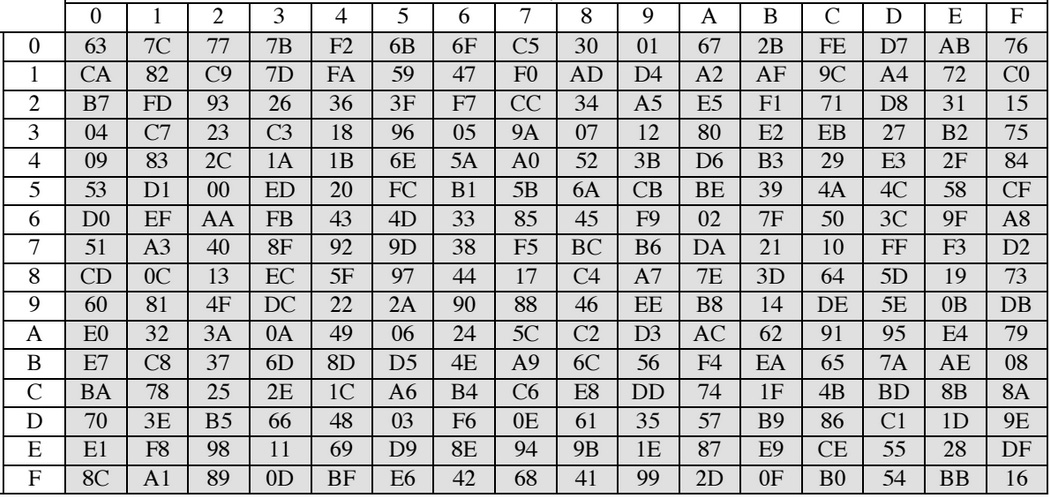
\includegraphics[width=\textwidth]{imagens/aes-subbyte.jpg}
  \caption{Tabela SubByte precomputada.}
  \label{fig:subbyte}
\end{figure}

Na fase de descriptografia do AES outra matriz e outra constante são aplicadas e em seguida é calculado o inverso em GF($2^8$) de forma a reverter o processo.

Na fase {\em MixColumn} são selecionados quatro bytes que são dispostos em um vetor para ser multiplicado por uma matriz, cada passo da multiplicação é calculado em $GF(2^8)$.


\begin{example}
  Considere que os bytes $B_0, B_5, B_{10}$ e $B_{15}$ foram selecionados.
  Fazemos a seguinte conta:

\begin{displaymath}
\left(\begin{array}{cccc}
02_{16} & 03_{16} & 01_{16} & 01_{16} \\
01_{16} & 02_{16} & 03_{16} & 01_{16} \\
01_{16} & 01_{16} & 02_{16} & 03_{16} \\
03_{16} & 01_{16} & 01_{16} & 02_{16} \\
\end{array} \right) 
\left( \begin{array}{c}
B_0\\ B_5\\ B_{10}\\ B_{15}\\\end{array} \right)
=
\left( \begin{array}{c}
C_0\\ C_1\\ C_2\\ C_3\\\end{array} \right)
\end{displaymath}  

Para facilitar as contas suponha que todos os bytes selecionados ($B_0, B_5, B_{10}$ e $B_{15}$)são $25_{16}$.
Neste caso precisamos calcular $02_{16} \cdot 25_{16}$ e $03 \cdot 25_{16}$:


\begin{eqnarray*}
  02_{16} \cdot 25_{16} & = & x(x^5 + x^2 + 1)\\
                      & = & x^6 + x^3 + x\\
  03_{16} \cdot 25_{16} & = & (x + 1)(x^5 + x^2 + 1)\\ 
                      & = & x^6 + x^5 + x^3 + x^2 + x + 1\\ 
\end{eqnarray*}

Neste caso, como todos $B_i$ são iguais, todos os $C_i$ também o são e são calculados da seguinte forma:

\begin{displaymath}
  \begin{array}{cccccccccc}
    01_{16} \cdot 25_{16} & = & & x^5 + & & & x^2 + & & 1\\
    01_{16} \cdot 25_{16} & = & & x^5 + & & & x^2 + & & 1\\
    02_{16} \cdot 25_{16} & = & x^6 + & & & x^3 + & & x & \\
    03_{16} \cdot 25_{16} & = & x^6 + & x^5 + & & x^3 + & x^2 + & x + & 1\\
    \hline
    C_i & = & & x^5 + & & & x^2 + &  & 1\\
  \end{array}
\end{displaymath}
\end{example}

No processo de descriptografia uma outra matriz é usada para calcular o {\em MixCloumn}, uma que reverte o que foi calculado neste passo.
%\chapter{Números Primos}
\label{cha:primos}

Para gerar uma chave no sistema RSA precisamos gerar primos grandes e aleatórios.
Para garantir que o número tera uma quantidade $n$ de bits sorteamos $p' \leftarrow \{0,1\}^{n-1}$ e acrescentar um bit $1$ à esquerda.
Caso o número não seja primos repetimos o processo.

Um importante resultado de Teoria dos Números chamado {\em Teorema dos Nùmeros Primos} estabelece que dado um número $n$ escolhido ao acaso, a chance de ele ser primo é $\frac{1}{ln(n)}$.
Se estamos buscando um número menor que $n$, precisamos em média chutar $ln(n)$ números até encontrar um primo ou metade disso se ignorarmos os pares.
Para cada tentativa, porém, precisamos verificar se o valor gerado é de fato primo.
A forma ingênua -- verificar cada um dos possíveis divisores -- é inviável.
Assim, precisamos utilizar algum método eficiente de verificação de primos.

A ideia que seguiremos é de procurar {\em testemunhas} de que um número é composto.
Por exemplo, o Teorema de Euller garante que para todo $a \in \mathbb{Z}_n^\star$ temos que $a^{\phi(n)} \equiv 1\ mod\ n$.
No caso em que $n$ é primo sabemos que $\phi(n) = n - 1$ que todo inteiro positivo $a$ é inversível em $\mathbb{Z}_n$.
Podemos então escolher $a \leftarrow \mathbb{Z}_n$ e fazer $a^{n-1}\ mod\ n$, se este valor for diferente de $1$ sabemos que $n$ não é primo.
Ou seja $a$ é uma testemunha de que $n$ não é primo.

Infelizmente existe uma infinidade de números compostos que não possuem esse tipo de testemunha.
Seja então $n - 1 = 2^ru$, temos que se $n$ é primo então a sequência $a^u, a^{2u}, \dots, a^{2^ru}$ em algum momento começa a produzir apenas $1$s.
Mais do que isso, com este teste todo número composto possui uma quantidade grande de testemunhas -- metade dos valores $a$ são testemunhas.
Assim, se testarmos $t$ valores de $a$ diferentes e escolhidos de maneira aleatória, a chance de todos os testes acusarem de maneira falsa que $a$ não é composto é $2^{-t}$.

Essa estratégia dá origem ao algoritmo de Miller-Rabin \cite{Miller75,Rabin80} que é o teste de primalidade mais usado hoje em dia:

\begin{codebox}
\Procname{$\proc{MillerRabin}(n, t)$}
\li \Comment Recebe $n, t \in \mathbb{Z}$
\li \Comment Devolve {\tt composto} se $n$ é composto
\li \Comment Devolve {\tt primo} se $n$ é primo com probabilidade $1 - 2^{-t}$
\li \If $n$ for par
\li   \Then \Return {\tt composto}
    \End
\li \If \proc{EhPotenciaPerfeita}(n)
%$n = n'^e$ para algum $n'$ e algum $e$
\li   \Then \Return {\tt composto}
    \End
\li  Calcule $r$ e $u$ tais que $n-1 = 2^ru$
\li \For $j = 1$ \To $t$
\li   \Do sorteia $a$ em $\{1, \dots, n-1\}$ 
\li   \For $i = 1$ \To $r-1$
\li     \Do \If $a^u \neq \pm 1\ mod\ n$ e $a^{2^iu} \neq -1\ mod\ n$
\li         \Then \Return {\tt composto}
            \End
      \End
    \End
\li \Return {\tt primo}
\end{codebox}

% Daqui para baixo ainda não está bom

Para mostrar que o algoritmo de Miller-Rabin é correto precisamos mostrar que pelo menos metade dos elementos em $\mathbb{Z}_n$ são testemunhas de que $n$ é primo.
Para tanto precisamos provar alguns resultados preliminares.


\begin{lemma}
  Se $H \subseteq G$ e $H$ é fechado então $H$ é um subgrupo de $G$. 
\end{lemma}
\begin{proof}
  Associatividade segue do fato de $H \subseteq G$ a existência de inverso e da identidade seguem do fecho.
\end{proof}

\begin{lemma}
Seja $H$ um subgrupo de $G$ tal que $H \neq G$, então $|H| \leq \frac{|G|}{2}$  
\end{lemma}
\begin{proof}
Como $H \neq G$ então existe $g \in G$ tal que $g \notin H$.
Considere o conjunto $\bar{H} := \{gh : h \in H\}$.

Se $gh_1 = gh_2$ então $h_1 = h_2$ (basta multiplicar os dois lados por $g^{-1}$), portanto, cada elemento distinto de $H$ corresponde a um elemento distinto em $\bar{H}$.
Ou seja, $|H| = |\bar{H}|$.

Agora suponha que $gh \in H$ para algum $h$.
Neste caso $gh = h'$ para algum $h' \in H$ e, portanto, $g = h'h^{-1}$.
Como $h', h^{-1} \in H$ e como $H$ é um grupo então $g \in H$, mas isso contradiz a definição de $g$ e portanto não existe $gh \in H$ para nenhum $h$.
Em outras palavras $\bar{H} \cap H = \emptyset$.

Juntando tudo temos que $H \subseteq G$ e $\bar{H} \subseteq G$ e, portanto, $|G| \geq |H| + |\bar{H}|$.
Como $|H| = |\bar{H}|$, concluimos que   $|G| \geq 2|H|$.
\end{proof}

Seja $i \in \{0, \dots r-1\}$ o maior inteiro tal que existe $a$ que não é testemunha e $a^{2^iu} \equiv -1\ mod\ n$.
Note que $i$ deve existir, pois $-1$ não é testemunha e $(-1)^{2^0u} \equiv -1\ mod\ n$ 
Vamos agora construir um conjunto $B$ que é um subgrupo de $\mathbb{Z}_n^\star$ e que $B \neq \mathbb{Z}_n^\star$:

\begin{displaymath}
  B := \{a : a^{2^iu} \equiv \pm 1\ mod\ n\}
\end{displaymath}

Seja $a$ um elemento que não é testemunha de que $n$ é primo i.e. $a^u \equiv 1\ mod\ n$ ou $a^{2^ju} \equiv -1\ mod\ n$ para algum $j \in \{0, \dots, r-1\}$.
No primeiro caso $a \in B$.
No segundo caso $j \leq i$.
Se $i =j$ então $a \in B$, caso contrário, $a^{2^iu} \equiv (2^{2^ju})^{2^{i-j}} \equiv 1\ mod\ n$ e temos que $a \in B$.
Concluímos que todo elemento que não é testemunha pertence a $B$.

Resta mostrar que $B$ é um subgrupo de $\mathbb{Z}_n^\star$ e que $B \neq \mathbb{Z}_n^\star$.
Para o primeiro basta notar que para quaisquer $a,b \in B$ temos que $a \cdot b \equiv (\pm 1)(\pm 1) \equiv \pm 1\ mod\ n$.
A demostração de que $B \neq \mathbb{Z}_n^\star$ é mais complicada e será omitida.



% concluimos que existem no máximo n/2 elementos de Z_n^* não são testemunhas de que n é primo
% provar a correção do algoritmo de Miller-Rabin

% mostrar o algoritmo EhPotenciaPerfeita e sua complexidade
\chapter{Sistemas Híbridos}
\label{cha:sistemas-hibridos}

Neste apêndice apresentamos duas construções concretas de sistemas híbridos: uma baseada no problema do logaritmo discreto e outra baseada no problema da fatoração.

\section{El Gammal}
\label{sec:el-gammal}

O principal inconveniente do sistema de El Gammal é que $M = \mathbb{G}$.
Ou seja, as mensagens devem ser elementos do grupo e não sequências arbitrárias de bits.
Não se deve restringir que mensagens os usuários devem ser capazes de trocar por conta de uma questão técnica como essa.
Uma forma de resolver esse problema é utilizando um sistema híbrido.

Uma forma de obter um sistema híbrido é simplemente usando o sistema de El Gamal para criptografar uma chave.
Ao invés disso, porém, podemos construir o seguinte KEM:

\begin{itemize}
\item $Gen(1^n) := \langle sk, pk \rangle$ em que e $\mathcal{G}(1^n) := \langle \mathbb{G}, g \rangle$, 
\begin{itemize}
\item $sk = \langle \mathbb{G}, g, x \rangle$ com $x \leftarrow \mathbb{Z}_n$ e
\item $pk = \langle \mathbb{G}, g, h, H \rangle$ com $H: \mathbb{G} \to \{0,1\}^{l(n)}$ e $h = g^x$
\end{itemize}
\item $Encaps(pk, 1^n) = \langle g^y, H(h^y)\rangle$ em que $y \leftarrow \mathbb{Z}_n$
\item $Decaps(sk, c) = H(c^x)$
\end{itemize}

A função $H$ é simplesmente uma função de hash.
Temos assim que $Decaps(sk, g^y) = H((g^y)^x) = H(g^{xy}) = k$, pois $k = H(h^y) = H(g^{xy})$.
É possível provar que este mecanismo de encapsulamento de chaves é tão seguro quanto o protocolo de Diffie-Helmann.
Usamos então $k$ como chave para criptografar uma mensagem com um sistema de criptografia simétrica para produzir um sistema híbrido.
Como já enunciamos, se o sistema de criptografia simétrico usado for seguro contra ataques ``ciphertext only'' então o sistema híbrido será seguro sob CPA.

\section{RSA}
\label{sec:rsa}

Como no caso da cifra de El Gamal, podemos construir um Mecanismo de Encapsulamento a partir do RSA.
A construção segue os seguintes passos:
\begin{itemize}
\item $Gen(1^n) := \langle sk, pk \rangle$ em que:
\begin{itemize}
\item $pk = \langle N, e \rangle$
\item $sk = \langle N, d' \rangle$ em que $d' = [d^n\ mod\ \phi(N)]$
\end{itemize}
\item $Encaps(pk, 1^n) = \langle c_{n+1}, k \rangle$ em que $c_1 \leftarrow \mathbb{Z}_N^\star$:
\begin{itemize}
\item $k_i := \textrm{\tt lsb}(c_i)$ e
\item $c_{i+1} := [c_i^e\ mod\ N]$
\end{itemize}
\item $Decaps(sk, c) = k'$ em que $c_1' = [c^{d'}\ mod\ N]$ e:
\begin{itemize}
\item $k_i := \textrm{\tt lsb}(c_i)$ e
\item $c_{i+1} := [c_i^e\ mod\ N]$
\end{itemize}
\end{itemize}

Em palavras, a ideia é criptografar o primeiro bit de $k$ usando o último bit de $[c^e\ mod\ N]$ para um $c$ escolhido aleatóriamente em $\mathbb{Z}_N^\star$.
O segundo bit de $k$ é computado usando o último de $[c^{e^2}\ mod\ N]$ e assim por diante.
Ao final o algoritmo $Encaps$ devole o $k$ obtido e $[c^{e^n}\ mod\ N]$.
Para decifrar partimos de $[c^{e^n}\ mod\ N]$ e elevamos a $d^n$ para recuperar o $c$ original e então repetimos exatamente o mesmo processo do algoritmo $Encaps$ para extrair cada um dos bits de $k$.

É possível mostrar que esta construção produz um KEM seguro e, portanto, pode ser usado para produzir um sistema híbrido seguro contra CPA como vimos.
Construir um sistema RSA seguro contra CCA requer uma série de modificações nos esquemas que vimos até aqui, cujos detalhes omitiremos.
A especificação de um sistema RSA seguro contra CCA foi formalizada em um sistema chamado {\tt RSA PKCS \#1 v2.0}.
\chapter{Grupos Cíclicos}
\label{cha:ciclicos}

No Capítulo \ref{cha:distribuicao-chaves} vimos que uma condição necessária para a segurança do protocolo de Diffie-Hellman é a dificuldade do problema do logaritmo discreto (DLog). 
Tanto o protocolo de Diffie-Hellman quanto o sistema de criptografia assimétrica de El Gammal assumem que podemos construir grupos cíclicos cujo problema DLog seja difícil.
Nesta seção apresentaremos duas construção de grupos cíclicos em que DLog é considerado difícil e ambas são usadas na prática.

\section{Grupos de ordem prima}
\label{sec:grupos-de-ordem}

O primeiro modelo parte de um teorema que estabelece que grupos com tamanho primo são necessariamente cíclicos e, além disso, qualquer elemento diferente da identidade é um gerador.

Vamos começar generalizando o Corolário \ref{cor:euler} do Teorema de Euler usado para provar a correção do algoritmo RSA.
Naquela situação estávamos usando um grupo específico, a saber, $\mathbb{Z}_n^\star$, mas o resultado vale para qualquer grupo finito: 


\begin{lemma}
   Seja $\mathbb{G}$ um grupo finito e $g \in \mathbb{G}$ um elemento de ordem $i$.
  Então para todo $x$ temos que $g^x = g^{[x\ mod\ i]}$.
\end{lemma}
\begin{proof}
Pelo algoritmo da divisão temos que $x = qi +r$ em que $r = [x\ mod\ i]$.
Portanto temos que:
\begin{displaymath}
  g^x = g^{qi + r} = g^{qi} \circ g^r = (g^i)^q \circ g^{[x\ mod\ i]} = g^{[x\ mod\ i]}
\end{displaymath}
\end{proof}

Agora podemos provar o seguinte teorema:

\begin{theorem}
  Se $\mathbb{G}$ é um grupo de ordem prima $p$ então $\mathbb{G}$ é cíclico e qualquer $g \in \mathbb{G}$ diferente de $1$ é um gerador.
\end{theorem}
\begin{proof}
  Seja $p = |\mathbb{G}|$ a ordem do grupo $\mathbb{G}$ e $i$ a ordem de um elemento qualquer $g \in \mathbb{G}$. 
  Pelo lema temos que $g^p = g^{[p\ mod\ i]}$ e pelo Teorema \ref{theo:gen-euler} temos que $g^p = 1$. 
  Como $[p\ mod\ i] < i$ e como, por definição, $i$ é o menor inteiro tal que $g^i = 1$ temos que $[p\ mod\ i] = 0$, ou seja, $i|p$.
  Mas, uma vez que $p$ é primo, temos que $i = 1$ ou $i = p$.
  O único elemento que tem ordem $1$ é a identidade, todos os demais tem ordem $p$ e, portanto, são geradores de $\mathbb{G}$.
\end{proof}

Esse resultado sugere que uma boa forma de encontrar grupos cíclicos é por buscando grupos de ordem prima.
Note, porém, que os candidatos naturais $\mathbb{Z}_p^\star$ tem ordem $p - 1$ o que quase nunca é primo\footnote{A única exceção é $p = 3$.}.
O que se costuma fazer é trabalhar com algum subgrupo de $\mathbb{Z}_p^\star$ de ordem prima.
O teorema a seguir, que não será provado, estabelece que se $p = qr + 1$ para algum $q$ primo, então o conjunto dos {\em $r$-ésimos resíduos módulo $p$}formam um grupo de tem tamanho $q$:

\begin{theorem}
Se $p = qr + 1$ e $p$ e $q$ são primos, então temos que
\begin{displaymath}
  \mathbb{G} = \{[h^r\ mod\ p] : h \in \mathbb{Z}_p\}
\end{displaymath}
é um subgrupo de $\mathbb{Z}_p^\star$ de ordem $q$.
\end{theorem}
   
Este teorema é o que garante a correção do seguinte algoritmo:

\begin{codebox}
\Procname{$\proc{GeradorDeGruposCiclicos}(1^n)$}
\li \Comment Recebe um parâmetro de segurança $1^n$ que estabelece $l = l(n)$
\li \Comment Devolve um grupo cíclico $\mathbb{G}$ cuja ordem é $q$ e um gerador $g$
\li escolhe aleatoriamente $q$ primo com $l$ bits
\li gera um primo $p$ tal que $q|(p-1)$
\li escolhe aleatoriamente $h \in \mathbb{Z}_p^\star$ tal que $h \neq 1$ 
\li $g \gets [h^{\frac{p-1}{q}}\ mod\ p]$
\li \Return $p, q, g$
\end{codebox}

O problema do logaritmo discreto para grupos gerados por esse algoritmo é considerado difícil.

\section{Curvas Elípticas}
\label{sec:curvas-elipticas}

Uma curva elíptica é formada por todos os pontos $(x,y)$ que satisfazem a seguinte equação, dados os parâmetro $a$ e $b$:

\begin{displaymath}
  y^2 = x^3 + ax + b 
\end{displaymath}

\begin{figure}[htbp]
  \centering
  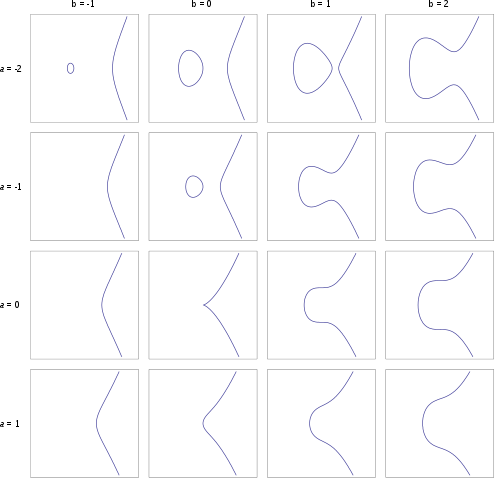
\includegraphics[width=.8\textwidth]{imagens/EllipticCurves.png}
  \caption{Curvas elípticas com diferentes parâmetros}
  \label{fig:curvas-elipticas}
\end{figure}

Podemos definir a adição de pontos em uma curva elíptica de maneira geometricamente natural.
A soma de dois pontos distintos é dada pelo ponto que intersecciona a reta que passa pelos dois (Figura \ref{fig:soma-eliptica} - quadro 1).
No caso extremo em que queremos somar o mesmo ponto duas vezes pegamos a reta tangente ao ponto e verificamos em qual ponto ela cruza com a reta (Figura \ref{fig:soma-eliptica} - quadro 2).
Nos casos degenerados em que a reta não cruza com a curva vamos atribuir um valor especial $0$ (Figura \ref{fig:soma-eliptica} - quadro 3).

\begin{figure}[htbp]
  \centering
  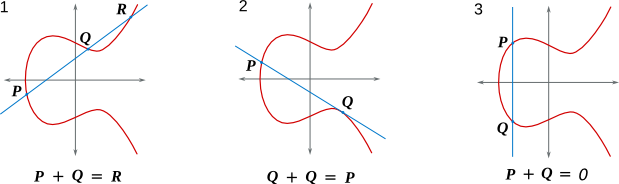
\includegraphics[width=\textwidth]{imagens/ECClines2.png}
  \caption{Soma de pontos em curvas elípticas}
  \label{fig:soma-eliptica}
\end{figure}

Algebricamente definimos a soma dos pontos da seguinte forma: $(x_1, y_1) + (x_2, y_2) = (x_3, y_3)$ tal que:

\begin{eqnarray*}
x_3 & = & s^2 - x_1 - x_2\\
y_3 & = & s(x_1 - x_3) - y_1  
\end{eqnarray*}

e $s$ (a inclinação da reta) na apresentação geométrica é dada por:

\begin{displaymath}
  s =\left\{
  \begin{array}{cl}
    \frac{y_2 - y_1}{x_2 - x_1} & \textrm{se os pontos são distintos}\\
    \frac{3x_1^2 + a}{2y_1} & \textrm{caso contrário}\\
  \end{array}\right .
\end{displaymath}


O conjunto $(\mathbb{R} \times \mathbb{R}) \cup \{0\}$ junto da operação que acabamos de definir é um grupo, porém, infinito.

Para nos mantermos no mundo dos grupos finitos estabeleceremos um número primo $p$ e faremos todas as contas acima módulo $p$ -- o que faz com que não sejamos mais capazes de expressar nossas contas de maneira geometricamente intuitiva.

Vamos então escrever o conjunto dos elementos de uma curva elíptica como:
\begin{displaymath}
  E(\mathbb{Z}_p) = \{(x,y) : x, y \in \mathbb{Z}_p \textrm{ e } y^2 \equiv x^3 + ax + b\ mod\ p\} \cup \{0\}
\end{displaymath}

O teorema a seguir nos dá algumas pistas sobre o tamanho deste conjunto:


\begin{theorem}[Hasse]
  Seja $p$ um número primo, então temos que:
\begin{displaymath}
  p + 1 - 2\sqrt{p} \leq |E(\mathbb{Z}_p)| \leq p + 1 + 2\sqrt{p} 
\end{displaymath}
\end{theorem}

Ou seja, o número de pontos em $E(\mathbb{Z}_p)$ é mais ou menos da mesma ordem do que $p$.
Podemos então construir o seguinte algoritmo análogo ao apresentado na seção anterior para computar um grupo cíclico:


\begin{codebox}
\Procname{$\proc{GeradorDeGruposCiclicos2}(1^n)$}
\li \Comment Recebe um parâmetro de segurança $1^n$
\li \Comment Devolve um grupo cíclico $\mathbb{G}$ cuja ordem é $q$ e um gerador $g$
\li escolhe aleatoriamente $p$ primo com $n$ bits
\li \While $q$ não for primo 
\li \Do escolha $a, b$ aleatoriamente em $\mathbb{Z}_p$ tal que $4a^3 + 27b^2 \neq 0\ mod\ p$
\li defina a curva elíptica $E(\mathbb{Z}_p)$
\li seja $q = |E(\mathbb{Z}_p)|$
\End
\li escolha um elemento qualquer $g \in E(\mathbb{Z}_p) \setminus \{0\}$
\li \Return $(a, b, p), q, g$
\end{codebox}

O logaritmo discreto de um grupo tal qual construído pelo algoritmo acima é considerado difícil.
\chapter{Algoritmo de Assinaturas Digitais}
\label{cha:dsa}

Neste apêndice nos aprofundaremos no tema das assinaturas digitais apresentando esquemas de identificação e o algoritmo DSA.

\section{Esquemas de Identificação}
\label{sec:esqu-de-ident}

Um esquema de identificação é um protocolo em que uma parte tem como objetivo provar sua identidade para a outra.
Chamamos de {\em provador} aquele que deseja provar sua identidade e {\em verificador} aquele que deseja verificá-la.
Assumimos que o verificador possui a chave pública do provador e vamos focar em protocolos com três interações e três algoritmos $langle \mathcal{P}_1, \mathcal{P}_2, \mathcal{V} \rangle$:
\begin{enumerate}
\item O provador usa $\mathcal{P}_1$ com sua chave secreta $sk$ para gerar uma {\em mensagem inicial} $I$ e um estado $st$ e envia $I$ para o verificador.
\item O Verificador escolhe um {\em desafio} $r$ aleatoriamente de um conjunto $\Omega_{pk}$ gerado a partida da chave pública do Provador e envia $r$  de volta.
\item O Provador usa $\mathcal{P}_2$ com entradas $sk$, $st$ e $r$ para gerar uma resposta $s$ que ele envia para o Verificador.
\item Por fim, o Verificador testa se $\mathcal{V}(pk, r, s)$ computa $I$.
\end{enumerate}

% DIAGRAMA!!!

A ideia por trás do esquema de identificação é que apenas que possui a chave secreta seria capaz de $s$ a partir do desafio $r$.
A mensagem $I$ e o estado $st$ servem para garantir que um adversário não copie os mesmos passos de identificação e seja bem sucedido.
Um esquema de identificação seguro deve garantir que seja computacionalmente inviável para um adversário enganar o sistema de identificação mesmo que ele observe vários processos similares.

% agora que isso ficou no apêndice talvez faça sentido colocar a parte da transformação de Fiat-Shamir

A partir de um sistema de identificação seguro é possível gerar um sistema de assinatura digital seguro usando a {\em transformação de Fiat-Shamir} \cite{Fiat87}. 
Na hora de assinar uma mensagem $I$ e $st$ são computados e calculamos $H(I, m)$ para gerar $r$ e usamos $r$, $sk$ e $st$ para gerar $s$.
A assinatura será exatamente o par $\langle r, s \rangle$.
O algoritmo de verificação deve rodar $\mathcal{V}$ com $pk$, $r$ e $s$ como entrada para produzir $I$ e então verifica-se se $H(I, m) = r$: 

\begin{itemize}
\item $Gen(1^n) := \langle sk, pk \rangle$ e assumimos que $H: \{0,1\}^* \to \Omega_{pk}$ é uma função de hash específica
\item $Sign(sk, m) = \langle r, s \rangle$ tal que
\begin{itemize}
\item $\mathcal{P}_1(sk) := \langle I, st \rangle$,
\item $r := H(I, m)$ e
\item $s := \mathcal{P}_2(sk, st, r)$
\end{itemize}
\item $Ver(pk, m, \langle r, s \rangle) = \left\{
    \begin{array}{lcl}
      1 & \textrm{se} & H(\mathcal{V}(pk, r, s), m) = r\\
      0 & \textrm{c.c.} &\\
    \end{array}
    \right.$
\end{itemize}

Considerando que o esquema de identificação $\langle \mathcal{P}_1, \mathcal{P}_2, \mathcal{V} \rangle$ seja seguro, podemos provar que o sistema de assinatura digital acima também é seguro, mas para esta prova é necessário supor não que $H$ seja resistente a colisões, mas que ele seja um {\em oráculo aleatório}, uma suposição muito mais forte e difícil de validar empiricamente.

\section{Algoritmo de Assinatura Digital (DSA)}
\label{sec:dsa}

O esquema de assinatura RSA depende da dificuldade do problema da fatoração.
Podemos também construir sistemas que dependem da dificuldade do problema do logaritmo discreto.
Este é o caso do popular esquema DSA e do ECDSA que usa curvas elípticas.
Antes de apresentar o sistema de assinatura digital, apresentaremos um esquema de identificação em que assumimos que a chave secreta é $x$ e a chave pública é $\langle \mathbb{G}, g, y, n \rangle$ com $\mathbb{G}$ um grupo cíclico, $g$ um gerador e $y = g^x$:

\begin{enumerate}
\item O Provador sorteia $k \leftarrow \mathbb{Z}_n^\star$ e envia $I := g^k$ para o Verificador.
\item O Verificador sorteia $a, r \leftarrow \mathbb{Z}_q$ como desafios e envia de volta.
\item O Provador envia $s := [k^{-1} \cdot (\alpha + xr)\ mod\ q]$ como resposta.
\item O Verificador aceita se $s \neq 0$ e $g^{\alpha s^{-1}} \cdot y^{rs^{-1}} = I$
\end{enumerate}

A probabilidade de $s = 0$ é desprezível.
Se assumirmos que $s \neq 0$ a correção do esquema segue, pois:
\begin{displaymath}
  g^{\alpha s^{-1}} \cdot y^{rs^{-1}} = g^{\alpha s^{-1}} \cdot g^{xrs^{-1}} = g^{(\alpha + xr)\cdot s^{-1}} = g^{(\alpha + xr)\cdot k \cdot (\alpha + xr)^{-1}} = g^k = I
\end{displaymath}

É possível provar que este esquema é seguro considerando que o problema do logaritmo discreto seja seguro.

Podemos transformar esse esquema de identificação em um sistema de assinatura usando a transformação de Fiat-Shamir, mas o popular esquema DSA segue um caminho um pouco diferente.
Assumiremos a existência de duas funções $H: \{0,1\}^* \to \mathbb{Z}_n$ e $F: \mathbb{G} \to \mathbb{Z}_n$:

\begin{itemize}
\item $Gen(1^n) = \langle sk, pk \rangle$ em que:
\begin{itemize}
\item $sk := x \leftarrow \mathbb{Z}_n$ e
\item $pk := \langle \mathbb{G}, g, y, n \rangle$ com $y = g^x$
\end{itemize}
\item $Sign(sk, m) = \langle r, s \rangle$ em que:
  \begin{itemize}
  \item $r := F(g^k)$ com $k \leftarrow \mathbb{Z}_n$ e
  \item $s := [k^{-1} \cdot (H(m) + xr)\ mod\ q]$ (sorteamos outro $r$ caso $s = 0$)
  \end{itemize}
\item $Ver(pk, m, t) := \left\{
    \begin{array}{lcl}
      1 & \textrm{se} & r = F(g^{H(m) \cdot s^{-1}} y^{r \cdot s^{-1}})\\
      0 & \textrm{c.c.} &\\
    \end{array}
    \right.$
\end{itemize}

A correção desse sistema é muito similar ao esquema de identificação apresentado anteriormente.
É possível provar sua segurança assumindo a dificuldade do problema do logaritmo discreto e tratando $H$ e $F$ como oráculos aleatórios.
No caso de $F$ isso é particularmente difícil de aceitar e não se conhece uma prova de segurança melhor do que essa até hoje.

\bibliography{ref}
\end{document}

% coisas que ficaram de fora
  % fatoração
  % teste de primalidade
  % criptoanálise diferencial
  % Zero knownledge proof of knowledge
% Ideia: OWF e mais esses 4 temas em curso de pós